\documentclass[bibliography=totocnumbered,a4paper,10pt,oneside]{scrbook}
\usepackage[utf8]{inputenc}
\usepackage{amsmath,amsthm, amssymb, latexsym}
\usepackage{epstopdf,graphicx}
\usepackage[hidelinks]{hyperref}
\usepackage{listings,xcolor,float,multirow}
\usepackage{array}
\usepackage{longtable}

\usepackage[a4paper, total={6in, 9in}]{geometry}
\usepackage{xspace}

\usepackage{pdfpages}

%==============%
%  Code Style  %
%==============%
\definecolor{serenity-green}{rgb}{0.1875,0.46875,0.0}
\lstset{
  basicstyle=\ttfamily,
  commentstyle=\color{gray}\ttfamily,
  columns=fullflexible,
  language=bash,
  frame=l,
  showstringspaces=false,
  backgroundcolor = \color{serenity-green!30}
}



%==========%
%  Macros  %
%==========%

\newcommand{
\serenity}{\textsc{Serenity}\xspace}

\newcommand{\ttt}[1]{%
  \begingroup\setlength{\fboxsep}{1pt}%
  \colorbox{serenity-green!30}{\texttt{\hspace*{2pt}\vphantom{(g}#1\hspace*{2pt}}}%
  \endgroup
}

%==============%
%  References  %
%==============%
\usepackage[backend=bibtex,
            sorting=none,
            style=chem-angew]{biblatex}
\addbibresource{SerenityUserManual.bib}

%============%
%  Document  %
%============%
\begin{document}
\thispagestyle{empty}
\begin{center}
\vspace*{1cm}

\includegraphics[width=0.95\textwidth]{./figs/SerenityLogo.png}\\
%{\Huge
% \textsc{Serenity}
%}\\
\vspace{2cm}
{\LARGE\textbf{
User Manual
}}\\
\vspace{1cm}
{\large\textbf{
Program Version: 1.6.0\\
Manual Generated: \today
}}\\
\vspace{2cm}
{\large\textbf{
The Serenity Developers$^{\dagger}$\footnote{Release Repository: \texttt{http://github.com/qcserenity/serenity}\\
                                             Developer Repository: \texttt{http://thclab.uni-muenster.de/serenity/serenity}}
\footnote{For questions and requests pertaining the manual please contact:\\ \texttt{serenity@uni-muenster.de}}
}}\\
\vspace{2cm}
{\large Manual layout by: \\
Jan P.\ Unsleber
}
\\[2ex]

$^{\dagger}$ Theoretische Organische Chemie,
Organisch-Chemisches Institut \\
and Center for Multiscale Theory and Computation,\\
Westf\"alische Wilhelms-Universit\"at M\"unster\\
Corrensstra{\ss}e 40, 48149 M\"unster, Germany\\[2ex]

\vfill
\end{center}
\newpage
\pagenumbering{Roman}
\setcounter{page}{1}
\tableofcontents

\newpage
\pagenumbering{arabic}
\setcounter{page}{1}
\numberwithin{equation}{subsection}
\chapter{Preface}
Subsystem and quantum embedding approaches are currently among the most quickly developing
methods in quantum chemistry. This is mostly due to their computational efficiency
and their easy interpretability in terms of intuitive, well-defined chemical subunits.
While the general idea of combining electronic-structure methods of different or the same
types for separate fragments is maybe straightforward, the practical execution of such
calculations can be a frustrating experience. The background is that such a combination
may require interfacing of different codes with limited interoperability through text files.
This strategy can be very successful, but usually also causes an overhead of work for the specific
interfaces needed. Moreover, it is vulnerable to (even slight) changes in the input/output
structure or working principles of the original programs. Even if all technical challenges
are dealt with, inexperienced users may find it hard to choose the optimum embedding approach
for a problem at hand, since comparison of different schemes can be very difficult.\\
\\
This was our motivation for developing a new quantum chemistry code that should give access
to a wide variety of quantum embedding approaches. This should allow for easy comparisons
of embedding schemes, as \serenity is written with a subsystem structure in mind right from
the beginning. Hence, it includes several possibilities for embedding calculations with
different ingredients. Its modular structure should make it easily extensible to upcoming
embedding features. As an open-source project, it may be tailored to user-specific requirements
whenever desired.\\
\\
The following manual shows how to use \serenity as a standalone program. Its usage as a
library is best explained through the source code (detailed manual
information may follow at a later point).


\chapter{Install}
Please read the following instructions carefully, these instructions can also be found in the \texttt{README.md} distributed with
the source code.

\section{Prerequisites}
The code has been tested and compiled on Linux with GCC/G++
(Versions 7 and newer) and Clang (Versions 8 and newer)
compilation with other compilers such as ICC should be
possible on Linux.\\
\\
Furthermore, the code has been compiled on macOS using Clang
but may experience problems depending on the CPU architecture.
Compilation with GCC on macOS should most likely also be possible.\\
\\
Compilation on and for Windows is not supported at the moment.
\\
The following programs/libraries must be available on your system:
\begin{itemize}
 \item CMake (Version $>=$ 3.12)
 \item Boost (for package managers: including boost-devel)
 \item OpenMP
 \item Eigen3
 \item HDF5 (Version $>=$ 1.10.1; including header files and cmake files)
 \item A recent GMP version, including C++ support (for libint2)
 \item The standard GNU tool chain (make, tar, autoconf, libtool)
\end{itemize}
The following libraries will be automatically downloaded and installed together
with \serenity (unless \texttt{SERENITY\_DOWNLOAD\_DEPENDENCIES=OFF} is set):
\begin{itemize}
 \item libint2 (Version 2.2.0-beta3, pre-configured and hosted at: \url{https://thclab.uni-muenster.de/serenity/libint})
 \item libecpint (The Serenity version is forked to: \url{https://github.com/qcserenity/libecpint})
 \item libxc (v6.1.0 from \url{https://gitlab.com/libxc/libxc})
 \item xcfun (The Serenity verison is forked to: \url{https://github.com/qcserenity/xcfun})
 \item GTest (Google Test and Google Mock)
\end{itemize}
The following libraries are optional and needed for additional features:
\begin{itemize}
 \item Intel MKL (for SMP parallel Eigen3 eigenvalue solvers)
 \item Doxygen (for the documentation)
 \item Python-devel (for the python wrapper)
 \item pybind11 (for the python wrapper)
 \item laplace-minimax (\url{https://github.com/bhelmichparis/laplace-minimax.git})
\end{itemize}

\section{Install Using CMake and Make}

Extract or pull the source code, then create a build directory:
\begin{lstlisting}
cd serenity
mkdir build
cd build
\end{lstlisting}
Then run cmake:
\begin{lstlisting}
cmake ..
\end{lstlisting}
To compile Serenity for your specific CPU architecture, you can add:
\begin{lstlisting}
cmake -DSERENITY_MARCH=native ..
\end{lstlisting}
(If the build folder is not located inside the main directory of \textsc{Serenity}
please adapt the path accordingly.)

Finally run make and make install to build the program:
\begin{lstlisting}
make
\end{lstlisting}
Please source serenity.sh located in the main folder to set all necessary environment
variables:
\begin{lstlisting}
cd ..
source serenity.sh
\end{lstlisting}
\section{Install Including Python Interface}
In order to activate the compilation of a Python interface to the code
a flag can be set as follows
\begin{lstlisting}
cmake -DSERENITY_PYTHON_BINDINGS=ON ..
\end{lstlisting}
additionally this and other flags can be toggled using `ccmake`
\begin{lstlisting}
ccmake ..
\end{lstlisting}
The wrapper will be build for the Python version that CMake finds first
In order to point CMake to a specific version of Python the following
option can be used:
\begin{lstlisting}
cmake -DPYTHON_EXECUTABLE=/usr/bin/python3 ..
\end{lstlisting}
The wrapper is shipped in form of a shared library (serenipy.so).
In order for Python to find this package the library folder has to be present
in the \texttt{PYTHONPATH} environment variable and the Serenity library has to be
present in a path searched by the system for shared libraries.
The latter is done when sourcing the \texttt{serenity.sh} script, the former requires
to un-comment one line in this file.
Afterwards the interface should importable as follows:
\begin{lstlisting}
python3
import serenipy as spy
\end{lstlisting}
\section{Tests}
Serenity comes with a decent set of unittests in order to run them source
the \texttt{serenity.sh} script and run
\begin{lstlisting}
PATH_TO_BUILD_DIR/bin/serenity_tests
\end{lstlisting}
Please use the complete path, or else GTEST might run into problems.

The Python wrapper comes with its own set of tests, these can be run using
\begin{lstlisting}
python -m unittest discover PATH_TO_SERENITY/src/python/tests
\end{lstlisting}
\section{Documentation}
After configuring the project using CMake it is possible to create the documentation
using:
\begin{lstlisting}
make doc
\end{lstlisting}
Then you can open up the doc/html/index.html in a browser.
The python wrapper is not featured inside the documentation.
Its documentation is available via pythons help() function,
which displays the build-in doc-strings.

\clearpage
\chapter{Text Input}

The input of \serenity has two main types of sections, the \ttt{system} blocks and the \ttt{task} blocks.
A chart depicting how \serenity handles input can be seen in Figure~\ref{fig:input}.
While the chart is already quite technical, it displays how to read the sectioned input.
Starting from the right, the main job of the program is to run tasks in a certain order.
These tasks can be related \textit{via} the systems they use, \textit{i.e.} a \ttt{MP2Task} will used
orbital data from a previous \ttt{SCFTask} if both of them are working with the same system.
Accordingly, the first part of the input has to be the system definitions which is followed by
a list of tasks to complete with these systems.
In a minimal case, the systems are just a geometry and a set of settings (such as charge, spin, basis set, and so on).
During the run these systems will be populated with more (calculated) data, such as orbitals, energies and electron densities.
This additional data can also be read from previous runs (see the following section).
Any feature that \serenity has is implemented as a task (or a part of a task).
For a list of available features/tasks, see Section~\ref{sec:tasks}.
\begin{figure}[h!]
\label{fig:input}
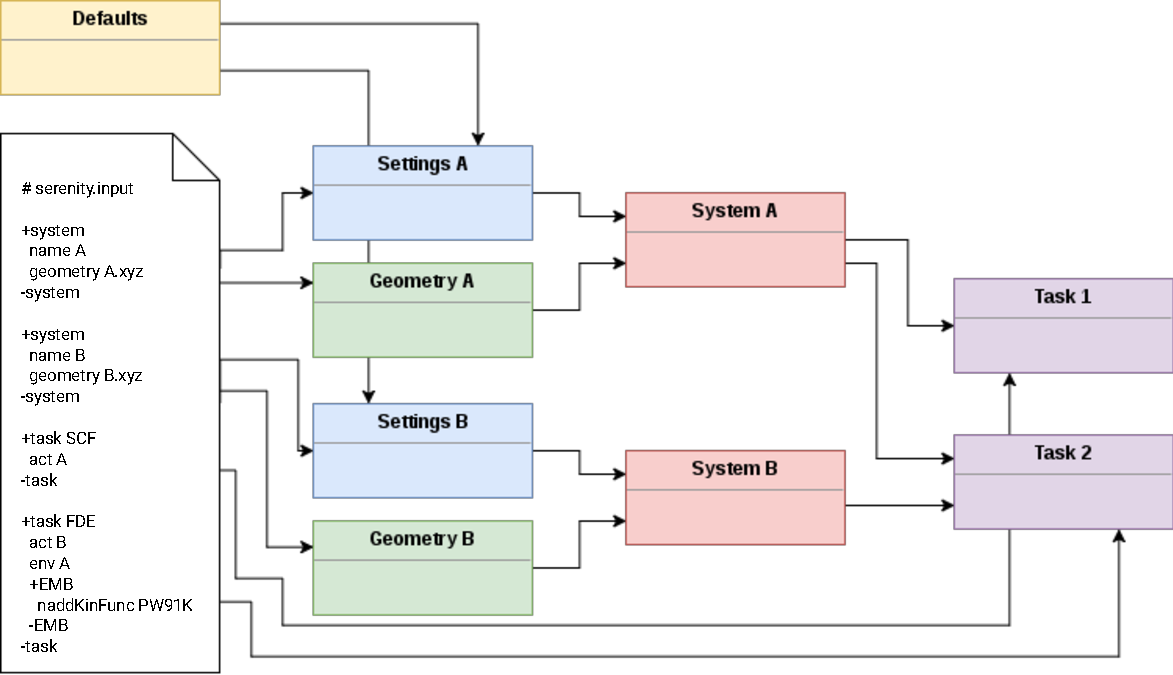
\includegraphics[width=0.95\textwidth]{./figs/SerenityInput.pdf}
\caption{Input flow of \serenity.}
\end{figure}\\
As stated above, the text input of \serenity is structured into blocks containing the keywords.
A keyword consists of a name and a value and is always given inside of a block.
Each keyword-value pair has to be given in one separate line.
As for the blocks, there are two main types, those are \ttt{system} and \ttt{task}.
A block in the {\serenity} text input is started by a \ttt{+<blockname>} and ended with a
\ttt{-<blockname>}.
The main blocks of a simple input might thus look like this:
\begin{lstlisting}
+system
 name water
 geometry ./water.xyz
 method dft
 +dft
  functional PBE
 -dft
-system

+task scf
  system water
-task
\end{lstlisting}
While there are many settings and thus many keywords, all of them are defaulted, and
each run of the program will create a file containing all settings (even the default ones)
for restart purposes.\\
The input accepts comments just like shell scripts.
Thus everything preceded  by a hash is not parsed.
This holds for entire lines but also for parts of a line.
\begin{lstlisting}
# not parsed
+system # also not parsed
 name test
 geometry test.xyz
 # you guessed it, this is also not parsed
-system
\end{lstlisting}
The entire input (with the exception of system names and path names) is case-insensitive.
Keywords could thus look like this:
\begin{lstlisting}
  gradients true
  funcTIONAL PbE0
  maxCycles 123
  NaMe water # note that the value of name is case sensitive
\end{lstlisting}
A list of values for a keyword can be parsed by enclosing them into curly brackets:
\begin{lstlisting}
  orbitals {1 2 3 4}
\end{lstlisting}
A list of settings (keywords) inside the \ttt{system} and \ttt{task} blocks will be
presented in the following two sections.

\newpage
\section{Systems}\label{sec:system}
Each system is defined by one system block, a system block contains general keywords and can contain one layer of sub-blocks.
All relevant keywords are discussed in this section.
\subsection{General Keywords}\label{sec:system:general}
\subsubsection{Example Input}
\begin{lstlisting}
  +system
    name methyl
    geometry methyl.xyz
    method HF
    charge 0
    spin 1
  -system
 \end{lstlisting}
\subsubsection{Basic Keywords}
\begin{description}
 \item [\texttt{name}]\hfill \\
   The system name.
 \item [\texttt{geometry}]\hfill \\
   The path to the geometry (.xyz). This or \ttt{load} has to be given.
   \item [\texttt{path}]\hfill \\
   The path to store HDF5 files.
   \item [\texttt{load}]\hfill \\
   The path to load HDF5 and settings files from. If this is given all other settings are replaced by the loaded settings. \serenity will search 
   for a directory with \ttt{name} at the given path.
   \item [\texttt{charge}]\hfill \\
   The charge of the system. Default is $0$.
   \item [\texttt{spin}]\hfill \\
   The spin of the system. Given as alpha spin electron excess. Default is $0$.
 \item [\texttt{scfmode}]\hfill \\
   The orbital mode of the SCF. Default is \ttt{RESTRICTED}. If \ttt{UNRESTRICTED} is chosen a unrestricted calculation is enforced.
  \item [\texttt{method}]\hfill \\
  The general electronic structure method for this system. By default \ttt{HF} (Hartree-Fock) is chosen. Other options are \ttt{DFT}.
\end{description}

The keywords given directly inside the system block and not within one of the nested blocks are presented
in this section.\\
A regular system will need both the \ttt{geometry} and also the \ttt{name} keyword.
Further keywords can be given if their values need to differ from the defaults.
A loaded system only needs the \ttt{load} keyword and a \ttt{name}.
All other keywords will be deduced from the stored settings.

\subsection{SCF Block}\label{sec:system:scf}
All settings available pertaining the SCF and its convergence are given in this sub-block of the system block.
\subsubsection{Example Input}
\begin{lstlisting}
  +system
    name methyl
    geometry methyl.xyz
    method HF
    charge 0
    spin 1
    +scf
      maxCycles 100
      damping dynamic
    -scf
  -system
 \end{lstlisting}
\subsubsection{Basic Keywords}
\begin{description}
 \item [\texttt{initialguess}]\hfill \\
   The initial guess for the electronic structure. Possible options are:\\
   \ttt{HCORE}: $h_{core}$ guess, i.e. ignoring electron-electron interactions.\\
   \ttt{EHT}: extended Hueckel theory guess.\\
   \ttt{ATOM\_SCF}: Attemps to load precalculated BHLYP/MINAO densities from disk and projects onto the basis set used in the calculation. If not found for a particular atom type
   or other problems occur, uses \ttt{ATOM\_SCF\_INPLACE} as a fall-back solution.\\
   \ttt{ATOM\_SCF\_INPLACE}: Generate the atomic densities on the fly with atom-wise SCFs in the basis of the calculation. Always starts from an Hcore guess with spherical densities.\\
   \ttt{SAP}: superposition of atomic potentials.\\
   The default is \ttt{ATOM\_SCF}. For atoms using effective core potentials, the \ttt{ATOM\_SCF\_INPLACE}
   guess is used as the default.
 \item [\texttt{damping}]\hfill \\
   The mode of damping of the new Fock matrix with the last one during the SCF.\\
   \ttt{NONE}: no damping.\\
   \ttt{SERIES}: damping value decreases in each step.\\
   \ttt{STATIC}: static damping value.\\
   \ttt{DYNAMIC}: dynamic damping value adjustment (see Ref.~\cite{cances2000can}).\\
   The default is \ttt{SERIES}.
   \item [\texttt{maxCycles}]\hfill \\
   Maximum number of SCF cycles. Default is $100$.
   \item [\texttt{energyThreshold}]\hfill \\
   Convergence criterion for the energy. Default is 5e-8.
   \item [\texttt{rmsdThreshold}]\hfill \\
   Convergence criterion for the density matrix. Default is 1e-8.
  \item [\texttt{diisThreshold}]\hfill \\
   The convergence criterion for the DIIS ([F,P]) error. Default is 5e-7.
   \item [\texttt{minimumLevelshift}]\hfill \\
   Minimum diagonal level-shift to be used. Default is $0.0$. Typical values are $0.3$ or $0.1$. Setting this to values larger than $0$ will
   help non-converging SCF procedures. However, it increases the number of iterations.
   \item [\texttt{rohf}]\hfill \\
   Can be used to invoke a restricted open-shell HF or KS calculation (ground-state). 
   Available are two flavors: \ttt{SUHF} [Chem. Phys. Lett. 183, 423 (1991)] and \ttt{CUHF} [J. Chem. Phys. 133, 141102 (2010)].
   Both are implemented as constrained UHF procedures. SUHF also requires a parameter (\texttt{suhfLambda}) which interpolates between
   UHF ($\lambda = 0$) and ROHF ($\lambda = \infty$). As a result, \ttt{SUHF} does not yield the \textit{exact} ROHF wavefunction with
   zero spin contamination in practice. \ttt{SUHF} may also struggle with convergence issues for $\lambda > 10$ and \ttt{CUHF} should
   basically always be preferred. Defaults to \ttt{NONE}.
   \item [\texttt{suhfLambda}]\hfill\\
   Scaling parameter for the SUHF procedure. Defaults to \ttt{0.01}.
   \item [\texttt{degeneracyThreshold}]\hfill\\
   Defaults to \ttt{0.0}. If set to something other than zero, fractionally occupies orbitals whose difference in eigenvalues is below this double.
\end{description}
\subsubsection{Advanced Keywords}
\begin{description}
    \item [\texttt{writeRestart}]\hfill \\
    Interval to write checkpoints during SCF. Default is $5$.
   \item [\texttt{seriesDampingStart}]\hfill \\
    Start value for the series damping. Default is $0.7$.
    \item [\texttt{seriesDampingEnd}]\hfill \\
    End value for the series damping. Default is $0.2$.
    \item [\texttt{seriesDampingStep}]\hfill \\
    Increment value for the series damping. Default is $0.05$.
    \item [\texttt{seriesDampingStart}]\hfill \\
    Start value for the series damping. Default is $0.7$.
    \item [\texttt{seriesDampingInitialSteps}]\hfill \\
    Number of initial steps without increment. Default is $2$.
    \item [\texttt{staticDampingFactor}]\hfill \\
    Damping value for the static damping. Default is $0.7$.
    \item [\texttt{endDampErr}]\hfill \\
    $\text{[F,P]}$ value at which the damping ends. Default is $0.05$.
    If the SCF has problems converging it may help to stop the damping at a lower error. However, this can
    increase the number of SCF iterations needed significantly.
    \item [\texttt{diisStartError}]\hfill \\
    $\text{[F,P]}$ value at which the DIIS starts. Default is $0.05$.
    \item [\texttt{diisMaxStore}]\hfill \\
    The number of Fock Matrices stored int the DIIS. Default is $10$. If oscillations in the SCF occur, it can
    help to change this number. Typical values are between $5$ and $15$.
    \item [\texttt{useLevelshift}]\hfill \\
    Use a level-shift for the diagonal elements of the virtual--virtual Fock matrix block. Default is \ttt{true}.
    \item [\texttt{useOffDiagLevelshift}]\hfill \\
    Use a scaling for the virtual--occupied Fock matrix block. Default is \ttt{false}.
    \item [\texttt{canOrthThreshold}]\hfill \\
    Minimum eigenvalue of the overlap matrix to be tolerated. Default is 1e-7. This eliminates linear dependencies
    in the basis set. The default threshold is quite conservative. Linear dependencies can lead to numerical instability
    for procedures that depend explicitly on the orbital coefficients, e.g. coupled cluster.
    \item [\texttt{useADIIS}]\hfill \\
    Use the A-DIIS\cite{hu2010} procedure at the beginning of the SCF. Default is \ttt{false}. This interpolation scheme
    includes an energy minimization criterion into the Fock-matrix update. The A-DIIS is supposed to be stable even for a
    bad initial guess. The A-DIIS is turned off automatically, when the DIIS procedure starts.
 \end{description}

\subsection{Basis Block}\label{sec:system:basis}
All settings available pertaining the usage and generation of basis sets.
The basis sets can be found in \texttt{data/basis}. These are not exclusive. Any folder with \textsc{Turbomole}
style basis sets can be given and every file can be added to it, given that the file names are spelled in
uppercase.

\subsubsection{Example Input}
\begin{lstlisting}
  +system
    name methyl
    geometry methyl.xyz
    method HF
    charge 0
    spin 1
    +basis
      label def2-SVP
    -basis
  -system
 \end{lstlisting}
\subsubsection{Basic Keywords}
\begin{description}
 \item [\texttt{label}]\hfill \\
 Basis set name. \serenity will search for a file with the given label in uppercase at the \ttt{basisLibPath}. Default is \ttt{6-31GS}.

\end{description}
\subsubsection{Advanced Keywords}
\begin{description}
    \item [\texttt{makeSphericalBasis}]\hfill \\
    Use spherical harmonics basis. Default is \ttt{true}. If \ttt{false}, a Cartesian basis set is constructed.
    \item [\texttt{basisLibPath}]\hfill \\
    Basis set file location (default taken from environment variable).
    \item [\texttt{auxJLabel}]\hfill \\
    Auxiliary basis set name for Coulomb interactions (RI). Default is \ttt{RI\_J\_Weigend}
    \item [\texttt{auxCLabel}]\hfill \\
    Auxiliary basis set name for Correlation interactions (RI). If none is given, \serenity will search for a
    basis-set file for the given basis with a filename \ttt{label}-RI-C.
    \item [\texttt{firstECP}]\hfill \\
    Atomic number threshold for the use of ECPs if available in the basis-set file. Default is $37$ (starting from the 5'th period).
    It is possible to manipulate/add the ECP definition to any basis-set file. For an example see the DEF2-SVP basis-set file.
    \item [\texttt{integralThreshold}]\hfill \\
    Threshold for the prescreening in integral evaluations. Default it is calculated as $1\cdot 10^{-8}/(3 M)$, where $M$ is
    the number of Cartesian basis functions.
    \item [\texttt{integralIncrementThresholdStart}]\hfill \\
    Initial integral prescreening threshold. Default is 1e-8.
    \item [\texttt{integralIncrementThresholdEnd}]\hfill \\
    Final integral prescreening threshold. Default it is equal to \texttt{integralThreshold}.
    \item [\texttt{incrementalSteps}]\hfill \\
    SCF-step interval to tighten the integral threshold by a factor of 100. Default is $5$.
    \item [\texttt{densFitJ}]\hfill \\
    The density fitting approach to be used for Coulomb contributions. By default the \ttt{RI} approximation is used. Furthermore, different approaches using the Cholesky decomposition can be chosen, namely the generic Cholesky decomposition \ttt{CD}, the atomic Cholesky decomposition \ttt{ACD} and the atomic-compact Cholesky decomposition \ttt{ACCD}. The full four center integrals may be used by selecting \ttt{NONE} for \ttt{densFitJ}.
    \item [\texttt{densFitK}]\hfill \\
    The density fitting approach to be used for exchange contributions. By default no density fitting is used. Besides that the \ttt{RI} approximation, different approaches using the Cholesky decomposition, namely the generic Cholesky decomposition \ttt{CD}, the atomic Cholesky decomposition \ttt{ACD} and the atomic-compact Cholesky decomposition \ttt{ACCD}, can be chosen.
    \item [\texttt{densFitLRK}]\hfill \\
    The density fitting approach to be used for long-range exchange contributions. By default no density fitting is used. Besides that the \ttt{RI} approximation, different approaches using the Cholesky decomposition, namely the generic Cholesky decomposition \ttt{CD}, the atomic Cholesky decomposition \ttt{ACD} and the atomic-compact Cholesky decomposition \ttt{ACCD}, can be chosen.
    \item [\texttt{densFitCorr}]\hfill \\
    The density fitting approach to be used to calculate correlation related contributions. By default the \ttt{RI} approximation is used. Furthermore, different approaches using the Cholesky decomposition can be chosen, namely the generic Cholesky decomposition \ttt{CD}, the atomic Cholesky decomposition \ttt{ACD} and the atomic-compact Cholesky decomposition \ttt{ACCD}. The full four center integrals may be used by selecting \ttt{NONE} for \ttt{densFitCorr}.
    \item [\texttt{cdThreshold}]\hfill\\
    Decomposition threshold for all Cholesky decomposition based methods. The default is \ttt{1e-6}.
    \item [\texttt{extendSphericalACDShells}]\hfill\\
    The scheme to generate complete spherical basis function products represented as a spherical function. \ttt{NONE} uses the pure product of the spherical basis functions. With the default setting \ttt{SIMPLE} a single additional basis function is added to account for missing contributions. Using \ttt{COMLETE} the full product is approximated.
    \item [\texttt{secondCD}]\hfill\\
    The decomposition threshold for the secondary decomposition. This threshold is used if an ACD or ACCD auxiliary basis set is generated for a spherical basis sets. The default value is \ttt{1e-8}.
    \item [\texttt{cdOffset}]\hfill\\
    Offset value used if an ACD or ACCD auxiliary basis set is generated for spherical basis sets. The default value is \ttt{1e-2}.
    \item[\texttt{intCondition}]
    Threshold to determine whether a four center integral should be cached or not.
    The caching criterion is based on the number of primitive  functions entering each basis function and their angular
    momentum. In general, integrals over highly contracted basis functions with low angular momentum are more likely to
    be cached. By default \ttt{-1} (no integral caching is used). For small to medium sized molecules
    (\emph{e.g.} up to 3000 basis functions) a threshold of \ttt{4} gives a balanced speed/memory-usage. The larger the
    threshold the more selective will the integral caching be.
 \end{description}

\subsection{Grid Block}\label{sec:system:grid}
All settings available to tune the generation of integration grids.
\subsubsection{Example Input}
\begin{lstlisting}
  +system
    name methyl
    geometry methyl.xyz
    method DFT
    charge 0
    spin 1
    +grid
      accuracy 5
      smallGridAccuracy 3
    -grid
  -system
 \end{lstlisting}
\subsubsection{Basic Keywords}
\begin{description}
  \item [\texttt{accuracy}]\hfill \\
  Overall accuracy of the integration grid. Range: 1-7, with 7 being most accurate.\\ Default is $4$.
 \item [\texttt{smallGridAccuracyel}]\hfill \\
 Accuracy for intermediate grids. Range: 1-7, with 7 being most accurate. Default is $2$.
\end{description}
\subsubsection{Advanced Keywords}
\begin{description}
    \item [\texttt{radialGridType}]\hfill \\
    Procedure how to combine atomic grids. Default is \ttt{SSF}.
    All options are:\\
    \ttt{BECKE}: the fuzzy cells\cite{beck1988}.\\ 
    \ttt{SSF}: the algorithm by Stratmann, Scuseria and Frisch\cite{stra1996}.\\ 
    \ttt{VORONOI}: sharp cuts between atoms.
    \item [\texttt{sphericalGridType}]\hfill \\
    Procedure how to construct the spherical part of the grid. Currently the only option and default is 
    the point distribution according to the work of Lebedev (\ttt{LEBEDEV}).
    \item [\texttt{gridPointSorting}]\hfill \\
    Enable or disable grid point sorting in order to enhance grid evaluation efficiency. Note that it should be
    set to \ttt{false} if using the \ttt{withAtomInfo} option within the \ttt{ExportGridTask}. Default is \ttt{true}.
    \item [\texttt{blocksize}]\hfill \\
    Size of blocked grid data  for parallelisation. Default is $128$.
    \item [\texttt{blockAveThreshold}]\hfill \\
    Threshold for average weights of blocks of data. Setting this to zero will increase accuracy and computational time of the numerical 
    integration for DFT type calculations. Default is 1e-11.
    \item [\texttt{basFuncRadialThreshold}]\hfill \\
    Threshold for the evaluation of basis functions on grid points. Setting this to zero will increase accuracy and computational time of the numerical 
    integration for DFT type calculations. Default is 1e-9.
    \item [\texttt{weightThreshold}]\hfill \\
    Threshold for grid point reduction. Default is 1e-14.
    \item [\texttt{smoothing}]\hfill \\
    Smoothing parameters for grid cells. Default is 2. This is the number of recursions on Becke's smoothing 
    function if \ttt{BECKE} is chosen as \ttt{gridType}, see Ref.~\cite{beck1988}.
 \end{description}


\subsection{DFT Block}\label{sec:system:dft}
The \ttt{DFT} block contains all options pertaining only DFT calculations.
Note that changes in this block do not automatically enable the \ttt{method dft}
keyword from the general system settings.
This keyword is still required in order to use \ttt{DFT} instead of the default \ttt{HF}.
\subsubsection{Example Input}
\begin{lstlisting}
  +system
    name methyl 
    geometry methyl.xyz
    method DFT 
    charge 0
    spin 1
    +dft
      functional PBE0
    -dft
  -system
 \end{lstlisting}
\subsubsection{Basic Keywords}
\begin{description}
  \item [\texttt{functional}]\hfill \\
  The exchange--correlation energy functional to use. A full list of functionals is given in the table below.
  The default is \ttt{BP86}.
 \item [\texttt{dispersion}]\hfill \\
 The version of Grimme's dispersion correction. The default is \ttt{NONE}. The options are:
 No correction (\ttt{NONE}), the third set of parameters (with zero damping, also called D3(0)) (\ttt{D3}),
 the third set of parameters (with zero damping, also called D3(0)) and 3 center correction term (\ttt{D3ABC}),
 the third set of parameters with Becke-Johnson damping (\ttt{D3BJ}),
 or the third set of parameters with Becke-Johnson damping and 3 center correction term (\ttt{D3BJABC}).
\end{description}

The following two tables list all possible exchange--correlation energy functionals and kinetic energy functionals.
The latter may be used for embedding calculations :
\begin{table}[H]\small \centering \begin{tabular}{|>{\ttfamily}c|l|>{\ttfamily}c|l|} \hline
\multicolumn{4}{|c|}{\textbf{Kinetic Energy Functionals}} \\ \hline
Functional & \multicolumn{1}{c|}{Notes} & Functional & \multicolumn{1}{c|}{Notes} \\ \hline
NONE     & No functional will be used. && \\ \hline
\hline \multicolumn{4}{|c|}{LDA} \\ \hline
TF       & & &\\ \hline
\hline \multicolumn{4}{|c|}{GGA} \\ \hline
PW91K    &                       &PBE2KS   & sDFT optimized PBE2K\\ \hline
LLP91K   &                       &PBE3K    & \\ \hline
LLP91KS  & sDFT optimized LLP91K &PBE4K    & \\ \hline
PBE2K    &                       &E2000K   & \\ \hline
\end{tabular}\end{table}
\begin{table}[H]\small \centering \begin{tabular}{|>{\ttfamily}c|l|>{\ttfamily}c|l|} \hline
\multicolumn{4}{|c|}{\textbf{Exchange--Correlation Energy Functionals}} \\ \hline
Functional & \multicolumn{1}{c|}{ Notes} & Functional & \multicolumn{1}{c|}{ Notes} \\ \hline
NONE     & No functional will be used. & & \\ \hline
\hline \multicolumn{4}{|c|}{LDA} \\ \hline
SLATER   & & LDA       & \\ \hline
VWN3     & & LDAERF    & \\ \hline
VWN5     & & LDAERF\_JT& \\ \hline
\hline \multicolumn{4}{|c|}{GGA} \\ \hline
OLYP     & &B97      & \\ \hline
BLYP     & &B97\_1   & \\ \hline
PBE      & &B97\_2   & \\ \hline
BP86     & &B97\_D   & \\ \hline
KT1      & &KT3      & \\ \hline
KT2      & &PW91     & \\ \hline
\hline \multicolumn{4}{|c|}{Hybrid} \\ \hline
PBE0     & & B3P86\_G & As implemented in Gaussian \\ \hline
B3LYP    & As implemented in Turbomole & BPW91    & \\ \hline
B3LYP\_G & As implemented in Gaussian & HF       & Performs a HF calculation.\\ \hline
B3P86    & As implemented in Turbomole & & \\ \hline
\hline \multicolumn{4}{|c|}{Double Hybrid} \\ \hline
B2PLYP   & &ROB2PLYP & \\ \hline
B2GPPLYP & &B2PIPLYP & \\ \hline
DSDBLYP  & &B2PPW91  & \\ \hline
DSDPBEP86& &DUT      & \\ \hline
B2KPLYP  & &PUT      & \\ \hline
B2TPLYP  & &&\\ \hline
\hline \multicolumn{4}{|c|}{Range-Separated Hybrid} \\ \hline
CAMB3LYP  &   & WB97X     & See \texttt{WB97}. \\ \hline
LCBLYP    &   & WB97X\_V  & See \texttt{WB97}. \\ \hline
LCBLYP\_47&   & WB97X\_D  & See \texttt{WB97}. \\ \hline
WB97      & Instabilities might occur in \texttt{libxc}. &           &           \\ \hline
\hline \multicolumn{4}{|c|}{Model Potential} \\ \hline
SAOP     & & &\\ \hline
\end{tabular}\end{table}


\subsection{PCM Block}\label{sec:system:pcm}

The PCM block contains all options for implicit solvent models. Note that this block can
be used not only in the system definition but in the task definition, too. If set for
a system, the PCM settings will apply to the system. For tasks the PCM settings will apply
to the task, which may affect multiple systems. For the embedding step of FDE-type
calculations any system-specific PCM-settings are ignored and only the task specific settings
are applied.

GEPOL-type\cite{Pascual-Ahuir1987} (solvent-excluded and solvent-accessible-surface) and
a Delley-type\cite{Delley2006} surface are available. Note, that the GEPOL-type surfaces
show discontinuities at the intersection between spheres surrounding atoms. The Delley-type
surface does not show these problems.

The parameters for the tabulated solvents are taken from
\url{{https://pcmsolver.readthedocs.io}}.
Note that this data is provided for convenience and may contain errors.

A detailed description of the implementation of the Delley-type surface is given in Sec.~\ref{sec:MolcSurface}.
Analytical gradients are implemented for single systems and CPCM only.

For single systems the calculation of a cavity formation energy using the Pierotti--Claverie scaled particle
theory formula\cite{langlet1988improvements} is possible. For the calculation of this energy a Van-der-Waals
type surface (DELLEY-type surface, Van-der-Waals-radii) is used.


\subsubsection{Example Input}
\begin{lstlisting}
  +system
    name water  
    geometry water.xyz
    method HF  
    charge 0
    spin 0
    +pcm 
      use true
      solverType CPCM 
      solvent ETHANOL
    -pcm 
  -system
 \end{lstlisting}
\subsubsection{Basic Keywords}
\begin{description}
  \item [\texttt{use}]\hfill \\
  If true, the implicit solvent model is used. The default is \ttt{false}.
 \item [\texttt{solverType}]\hfill \\
 The type of solver continuum model to be used. \ttt{CPCM} selects the continuum-like PCM and 
 \ttt{IEFPCM} selects the integral equation formalism variant of PCM. \ttt{CPCM} is the default.
 \item [\texttt{solvent}]\hfill \\
 Select a predefined and tabulated solvent. The default is \ttt{WATER}. All options are given in the table below.
 The manual solvent definition can be triggered by selecting \ttt{EXPLICIT} as the solvent. If done so, the keywords 
 \ttt{eps} (static permittivity) and \ttt{probeRadius} (solvent probe radius) have to be set manually.
 \item [\texttt{cavityFormation}]\hfill \\
 Enable the calculation of a cavity formation energy using scaled particle theory. The defualt
 is \ttt{false}.
\end{description}
\subsubsection{Advanced Keywords}
\begin{description}
    \item [\texttt{scaling}]\hfill \\
    If true, the atom-radii used for the cavity construction are scaled by a factor of $1.2$. This is commonly done 
    when using the \texttt{BONDI} (VdW radii) of the atoms for cavity construction. For the \ttt{UFF} radii set it is 
    adviced to turn this scaling off. The default is \ttt{true}.
    \item [\texttt{cavity}]\hfill \\
    The type of cavity used with the PCM. The default is a Delley-type cavity (\ttt{DELLEY}). Other options are 
    a primitive version of the GEPOL cavity which is available as a solvent excluded surface \ttt{GEPOL\_SES} and 
    solvent accessible surface \ttt{GEPOL\_SAS}.
    \item [\texttt{radiiType}]\hfill \\
    The atomic radii-set to be used in the cavity construction. The default is the Bondi-Mantina radii set \ttt{BONDI}.
    Note that not for all atoms radii are tabulated in this set. For the \ttt{UFF} radii set all atoms are supported.
    If the \texttt{UFF} radii set is used, it is adviced to select \ttt{scaling} as \ttt{false}.
    \item [\texttt{minDistance}]\hfill \\
    Minimum distance tolerated between surface grid points in Bohr. The default is $0.2$. This prevents singularities
    for extremely close points.
    \item [\texttt{minRadius}]\hfill \\
    Minimal radius in Bohr for additional spheres not centered on atoms (GEPOL-type surfaces only). The default is $0.377$ au.
    \item [\texttt{correction}]\hfill \\
    Correction $k$ for the apparent surface charge scaling factor in the CPCM. The default is $0.0$. In the related 
    COSMO solvation model $k$ is chosen as $0.5$. This has little effect on solvent with a high static permittivity
    but may be important for others.
    \item [\texttt{probeRadius}]\hfill \\
    Radius in Bohr of the spherical probe approximating a solvent molecule. The default is $1.0$. This is only used if
    the explicit solvent definition is used by selecting \ttt{solvent=EXPLICIT}. Otherwise the tabulated
    data is used.
    \item [\texttt{eps}]\hfill \\
    The static dielectric permittivity of the medium. The default is $1.0$. This is only used if 
    the explicit solvent definition is used by selecting \ttt{solvent=EXPLICIT}. Otherwise the tabulated
    data is used.  
    \item [\texttt{patchLevel}]\hfill \\
    Wavelet cavity mesh patch level for GEPOL cavities. The default is $0$. This increases the resoluation of the 
    GEPOL-type cavity at the intersection between spheres.
    \item [\texttt{overlapFactor}]\hfill \\
    Maximum ratio of a new sphere to be allowed to be covered within the already present ones. This is only used for 
    GEPOL-type surfaces. The default is $0.7$.  
    \item [\texttt{lLarge}]\hfill \\
    Angular momentum used for the spherical grid construction for non-hydrogen atoms for DELLEY-type surfaces. The default
    is $7$, which corresponds to 110 spherical grid points for each  non-hydrogen atom.
    \item [\texttt{lSmall}]\hfill \\
    Angular momentum used for the spherical grid construction for hydrogen atoms for DELLEY-type surfaces. The default
    is $4$, which corresponds to 50 spherical grid points for each hydrogen atom.
    \item [\texttt{alpha}]\hfill \\
    The sharpness parameter for the molecular surface model function for DELLEY-type surfaces. The default
    is $50$, which corresponds to fairly sharp surfaces. Since the model employes an exponential 
    molecular surface model function, results are relatively stable with vaiation of the parameter. The surface 
    will typically become obese for values smaller than $10$, which leads to a lowered dielectric interaction with 
    the continuum.
    \item [\texttt{projectionCutOff}]\hfill \\
    The cut-off for the projection to the molecular surface for DELLEY-type surfaces. Each atom-wise grid 
    point is projected to the molecular surface. If the molecular surface is too far away, the grid point is 
    assumed to be unimportant and covered within the molecule. The value is given in atomic units. Its default is 
    $5.0$.
    \item [\texttt{oneCavity}]\hfill \\
    Only cavity points connected to the point with the most extreme
    x-coordinate are kept after cavity construction. Two points are connected if they are within
    $connectivityFactor\times probeRadius$ from another. This can be used to eliminate cavity points within a 
    moleular cluster. The default is \ttt{false}.
    \item [\texttt{connectivityFactor}]\hfill \\
    The scaling factor for point connection. The default is $2.0$. Increase this for low
    resolution cavities. This is only used for \ttt{oneCavity=true}.
    \item [\texttt{numberDensity}]\hfill \\
    The number density (in a.u.) of the solvent. The default is $1.0$. This is only used if 
    \ttt{solvent=EXPLICIT} and \ttt{cavityFormation=true} are given.
    \item [\texttt{temperature}]\hfill \\
    The temperature used in the scaled particle theory treatment of the cavity formation. The
    default is $298.15$. This is only used if \ttt{cavityFormation=true} is given.
    \item [\texttt{cavityProbeRadius}]\hfill \\
    The probe radius used for the calculation of the cavity formation energy. The default is $5.0$.
    This is only used if \ttt{solvent=EXPLICIT} and \ttt{cavityFormation=true} are given. 
 \end{description}

\begin{table}[H]\small \centering \begin{tabular}{|>{\ttfamily}c|l|} \hline 
\multicolumn{2}{|c|}{\textbf{PCM Solvents}} \\ \hline
Solvent & \multicolumn{1}{c|}{ Keyword} \\ \hline 
Water               & WATER, H2O \\ \hline 
Propylenecarbonate  & PROPYLENECARBONATE, C4H6O3 \\ \hline 
Dimethylsulfoxide   & DIMETHYLSULFOXIDE, DMSO, C2H6OS \\ \hline 
Nitromethane        & NITROMETHANE, CH3NO2 \\ \hline 
Acetonitrile        & ACETONITRILE, CH3OH \\ \hline 
Methanol            & METHANOL, MEOH, CH3OH \\ \hline 
Ethanol             & ETHANOL, ETOH, CH3CH2OH  \\ \hline 
Acetone             & ACETONE, C2H6CO \\ \hline 
1,2-Dichlorethane   & 1,2-DICHLORETHANE, DICHLORETHANE, C2H4CL2  \\ \hline 
Methylenechloride   & METHYLENECHLORIDE, CH2CL2  \\ \hline
Tetrahydrofurane    & TETRAHYDROFURANE, THF, C4H8O  \\ \hline 
Aniline             & ANILINE, C6H5NH2 \\ \hline 
Chlorobenzene       & CHLOROBENZENE, C6H5CL \\ \hline 
Chloroform          & CHLOROFORM, CHCL3 \\ \hline 
Toluene             & TOLUENE, C6H5CH3 \\ \hline 
1,4-Dioxane         & DIOXANE, C4H8O2, 1,4-DIOXANE \\ \hline 
Benzene             & BENZENE, C6H6 \\ \hline 
Carbontetrachloride & CARBONTETRACHLORIDE, CCL4 \\ \hline 
Cyclohexane         & CYCLOHEXANE, C6H12 \\ \hline 
N-Heptane           & N-HEPTANE, C7H16 \\ \hline 
Explicit            & EXPLICIT (triggers explicit solvent definition) \\ \hline 
\end{tabular}\end{table}

\subsection{EField Block}\label{sec:system:efield}
The \ttt{EField} block contains options regarding external electric fields. Currently,
two strategies for using electric fields can be chosen. First, a molecular system is placed between 
two circular plates consisting of opposing point charges which will be referred to as numerical
electric field. The algorithm used for constructing these capacitor plates loosely resembles the
method used in TITAN~\cite{stuyver2020}.
Second the so-called analytical electric fields are produced by incorporating
dipole integrals into the Core Hamiltonian.
Parameters of this algorithm can be adjusted here.
\subsubsection{Example Input}
Numerical efield:
\begin{lstlisting}
  +system
    name water 
    geometry water.xyz
    +efield
      use true
      pos1 {0.0 0.0 0.0}
      pos2 {0.0 0.0 1.0}
      distance 50
      nRings 50
      fieldStrength 1e-3
      nameOutput efieldplate
    -efield
  -system
 \end{lstlisting}
Analytical efield:
\begin{lstlisting}
  +system
    name water 
    geometry water.xyz
   +efield
     use true
     analytical true
     pos1 {0.0 0.0 0.0}
     pos2 {0.0 0.0 1.0}
     fieldStrength 1e-3
   -efield
 -system
\end{lstlisting}
\subsubsection{Basic Keywords}
\begin{description}
  \item [\texttt{use}]\hfill \\
  A boolean to trigger the electric field usage.
  The default is \ttt{false}.
  \item [\texttt{analytical}]\hfill \\
  A boolean to trigger the analytical electric field usage. If chosen \ttt{false}
  the numerical field is used.
  The default is \ttt{false}.
 \item [\texttt{pos1}]\hfill \\
  The electric field will point from \ttt{pos1} to \ttt{pos2}, \emph{i.e.}
  the positively charged plates will appear on the side of \ttt{pos1} and 
  the negatively charged plates will appear on the side of \ttt{pos2}.
  The default for \ttt{pos1} is \ttt{\{0.0 0.0 0.0\}}.
 \item [\texttt{pos2}]\hfill \\
  See \ttt{pos1}.
  The default for \ttt{pos2} is \ttt{\{0.0 0.0 1.0\}}.
 \item [\texttt{distance}]\hfill \\
 Specifies the distance between the center point of the capacitor plates and 
 the position in the middle between \ttt{pos1} and \ttt{pos2} in \AA. The default is \ttt{50.0}.
 \item [\texttt{nRings}]\hfill \\
 The capacitor plates are organized in rings made up of point charges. This keyword specifies the
 number of rings to construct. The default is \ttt{50}.
 \item [\texttt{radius}]\hfill \\
 The radius between two adjacent rings in \AA. The default is \ttt{1.0}.
 \item [\texttt{fieldStrength}]\hfill \\
 The strength of the electric field in atomic units. Note that 1 a.u. is
 approximately equivalent to $5.14\cdot 10^{11}~\mathrm{V/m}$. The default is \ttt{1e-3}.
 \item [\texttt{outputName}]\hfill \\
 If specified, the electric field plates will be written to disk as an xyz-file. Negative
 charges will be printed as boron atoms (B), positive charges as xenon atoms (Xe).
\end{description}

\clearpage
\section{Tasks}
\label{sec:tasks}
The task block accepts different options depending on the task to be run.
These task specific options, as well as the options common to all tasks will be listed and explained
in the following section.\\
\\
The general form of a task block is the following.
Each task block is opened by a \ttt{+task} statement followed by the name of the
task to be run and is ended by a \ttt{-task} statement.\\
Furthermore each task block accepts three types of systems. Supersystem (keywords: \ttt{super}),
Active  systems (keywords: \ttt{system}, \ttt{active}, \ttt{act}) and environment systems
(\ttt{environment}, \ttt{env}) their meaning changes depending
on the task type. Additionally a print level (keywords: \ttt{printLevel}) and timings
print level (keyword: \ttt{timingsPrintLevel}) are available
for every task. The effect of the print levels will depend on the task. More information
is given in Section~\ref{sec:tasksPrintLevels}.
The exact meaning of active versus environment system will be given in this sections
for each task specifically.
A minimal task block for a SCF calculation could look like this:
\begin{lstlisting}
+task scf
  system water
-task
\end{lstlisting}
Note that some tasks may use a block structure similar to the system settings.
The blocks are opened and closed in the same way as before. The input for an
FDE calculation for two water molecules with the Huzinaga operator and the
PBE functional for the exchange--correlation interaction may look like this:
\begin{lstlisting}
+task FDE
  act waterA
  env waterB
  +emb
    naddXCFunc PBE
    embeddingMode HUZINAGA
  -emb
-task
\end{lstlisting}
Possible blocks are listed in the respective task documentation and their
structure shown in the following sections starting with~\ref{sec:scb:emb}.

\subsection{General Keywords}
\label{sec:tasksPrintLevels}
The following keywords are present, and can be changed in all tasks, regardless
of the other keywords present.
\begin{description}
  \item [\texttt{printLevel}]\hfill \\
Changing the print level may result in additional output which is indented by
a set of characters in order to allow for easy searches. Furthermore, the number
of eigenvalues printed to the output after converging a SCF calculation depends
on the print level.
The print levels for every task and their effects are:
\begin{table}[H]\small \centering \begin{tabular}{|>{\ttfamily}c|>{\ttfamily}c|l|}\hline
   & \multicolumn{1}{c|}{Indent}&\multicolumn{1}{c|}{Number printed eigenvalues}\\\hline
  \texttt{MINIMUM}          &       & HOMO-LUMO gap    \\\hline
  \texttt{NORMAL }[Default] &       & HOMO-9 to LUMO+9 \\\hline
  \texttt{VERBOSE}          & ==V== & 0 to LUMO+9      \\\hline
  \texttt{DEBUGGING}        & ==D== & ALL              \\\hline
\end{tabular}
\end{table}
\item [\texttt{timingsPrintLevel}]\hfill \\
   The amount of timings that will be printed to the output. This settings is closer to a
   debug/developer setting, yet it may also be interesting for an experienced user.
   The default value is $1$, a value of $0$ will remove many timings, higer
   values than $1$ may add additional timings.
\end{description}
\subsubsection{Example Input}
\begin{lstlisting}
  +task SCF
    actsystem water
    printLevel debugging
    timingsPrintLevel 0
  -task
\end{lstlisting}


\subsection{Common Sub-Block: Embedding Settings}
\label{sec:scb:emb}
The \texttt{EMB} block contains all settings for embedding calculations. Be aware: some defaults may vary between the tasks.
\subsubsection{Example Input}
\begin{lstlisting}
  +task fat
    system ammonia1
    system ammonia2
    +emb
      naddXcFunc PW91
      embeddingmode NADDFUNC
    -emb
  -task
\end{lstlisting}
\subsubsection{Basic Keywords}
\begin{description}
  \item [\texttt{embeddingMode}]\hfill \\
    The type of embedding to be done. Possible options are:
    \ttt{NONE}, no treatment of Pauli-repulsion.
    \ttt{NADD\_FUNC}, the standard subsystem DFT formalism, employing two non-additive density functionals.
    This options is the default in most cases.
    \ttt{LEVELSHIFT}, a projector based embedding using only one non-additive density functional for exchange
    and correlation. This method was introduced by Manby and Miller.
    \ttt{RECONSTRUCTION}, embedding using potential reconstruction techniques.
    Furthermore there are three more projector based embedding techniques that use only one non-additive
    density functional for exchange and correlation. These can be used with the keywords \ttt{HUZINAGA} and
    \ttt{FERMI\_SHIFTED\_HUZINAGA} or \ttt{FERMI}, as well as \ttt{HOFFMANN}.
    Note that depending on the actual task. The selection of embedding modes can be limited. As an example,
    the calculation of nuclear gradients is only possible for \ttt{NADD\_FUNC} type calculations.
  \item [\texttt{naddXCFunc}]\hfill \\
    The exchange--correlation functional to be used in the evaluation of the non-additive term arising in the
    subsystem DFT formalism. The list of available functional can be found in Section~\ref{sec:system:dft}.
    Note that double hybrid functional are not fully supported yet. 
  \item [\texttt{naddKinFunc}]\hfill \\
    The kinetic energy functional to be used in the evaluation of the non-additive term arising in the
    subsystem DFT formalism. The list of available functional can be found in Section~\ref{sec:system:dft}.
  \item [\texttt{levelShiftParameter}]\hfill \\
    When using \ttt{embeddingMode LEVELSHIFT} this parameter determines the magnitude by which the environment
    orbitals are shifted. The default value is \ttt{1e-6}.
  \item [\texttt{dispersion}]\hfill \\
    The type of dispersion interaction correction to emply for the calculation of interactions between the
    embeded systems.
\end{description}
\subsubsection{Advanced Keywords}
\begin{description}
  \item [\texttt{calculateMP2Correction}]\hfill \\
    A flag to turn off the evaluation of the MP2 correction for double hybrid functionals. By default it will
    be calculated.
  \item [\texttt{fullMP2Coupling}]\hfill \\
    If true, the MP2 contribution of the non-additive exchange-correlation energy for double hybrids captures
    the effect of environment orbital pairs on the active-pair amplitudes. By default \ttt{False}.
  \item [\texttt{longRangeNaddKinFunc}]\hfill \\
    Long-range non-additive kinetic energy for hybrid methods. Only used if \ttt{embeddingMode} is one of
    the projection based methods is used. This option is intended to manly be used in conjunction with
    \ttt{embeddingMode LEVELSHIFT}. By default this option is disabled\\ (\ttt{longRangeNaddKinFunc NONE}).
    For a list of posssible functionals see the kinetic energy functionals in Section~\ref{sec:system:dft}.
  \item [\texttt{borderAtomThreshold}]\hfill \\
    The Mulliken population threshold used to determine if an orbital is considered ``distant'' or not.
    Only used in hybrid functional/projection schemes. By default \ttt{0.02}.
  \item [\texttt{basisFunctionRatio}]\hfill \\
    The minimum ratio of retained basis function shells needed in order to consider an atom to be not
    ``distant''. Only used in hybrid functional/projection schemes. By default \ttt{0.0}.
  \item [\texttt{truncateProjector}]\hfill \\
    A flag to truncate the projection operator in bottom-up calculations. Only used if any kind of projection
    technique is used. By default \ttt{False}.
  \item [\texttt{projecTruncThresh}]\hfill \\
    Total overlap threshold for the truncation of the projection operator. Only used if \\
    \ttt{truncateProjector true} and hence only usefull in any kind of projection technique.
    By default \ttt{1.0e+1}.
  \item [\texttt{fermiShift}]\hfill \\
    An optional shift for the Huzinaga operator. Only used if\\ \ttt{embeddingMode FERMI\_SHIFTED\_HUZINAGA} is
    used. By default \ttt{1.0}.
  \item [\texttt{carterCycles}]\hfill \\
    Number of update cycles for the Zhang-Carter potential reconstruction. Only relevant if
    \ttt{embeddingMode RECONSTRUCTION} is used.
  \item [\texttt{potentialBasis}]\hfill \\
    The label of the basis set used for the potential reconstruction. Only relevant if\\
    \ttt{embeddingMode RECONSTRUCTION} is used.
  \item [\texttt{singValThreshold}]\hfill \\
    Threshold for the singular value decomposition in potential reconstruction. Only relevant if
    \ttt{embeddingMode RECONSTRUCTION} is used.
  \item [\texttt{lbDamping}]\hfill \\
    Damping for the density update in the van Leeuwen--Barends potential reconstruction. Only relevant if
    \ttt{embeddingMode RECONSTRUCTION} is used.
  \item [\texttt{lbCycles}]\hfill \\
    Number of update cycles for the van Leeuwen--Barends potential reconstruction. Only relevant if
    \ttt{embeddingMode RECONSTRUCTION} is used.
  \item [\texttt{smoothFactor}]\hfill \\
    The smoothing factor for the potential reconstruction. Only relevant if\\
    \ttt{embeddingMode RECONSTRUCTION} is used.
\end{description}

\subsection{Common Sub-Block: Local Correlation Settings}
The \texttt{LC} block contains all settings for calculations based on local-correlation schemes.
Some defaults may vary between the tasks and the pair natural orbital-(PNO-)macro flag
(\ttt{pnoSettings}) used (\ttt{TIGHT}, \ttt{NORMAL} or \ttt{LOOSE}).
All defaults set by the PNO-macro flag \ttt{pnoSettings} can be overwritten.

\subsubsection{Example Input}
\begin{lstlisting}
  +task MP2
    system water  
    mp2Type local
    +lc 
      pnoSettings TIGHT    #the PNO-macro flag
      pnoThreshold 3.3e-8  #overrides the value given by the macro
      useFrozenCore true
    -lc 
  -task
 \end{lstlisting}
\subsubsection{Basic Keywords}
\begin{description}
  \item [\texttt{pnoSettings}]\hfill \\
  The PNO-macro flag. This flag can be used to manipulate several settings at once. The default value is
  \ttt{NORMAL}. The other options are \ttt{LOOSE} and \ttt{TIGHT} with looser and tighter thresholds
  respectively. The actual values associated with this setting are given below and are different for
  coupled-cluster and MP2.
 \item [\texttt{useFrozenCore}]\hfill \\
 If true, the frozen core approximation is used. Frozen core orbitals are determined by the orbital energy
 threshold \texttt{energyCutOff}. By default, no frozen-core approximation (\ttt{false}) is used. Note
 that using a frozen-core approximation requires that the core and valence orbitals have been localized
 independently.
 \item [\texttt{linearScalingSigmaVector}]\hfill \\
 If true, the integrals required for the sigma vector construction in DLPNO-CCSD are calculated directly from
 intergrals calculated during the main integral transformation. This requires slightly more memory, however,
 the amplitude optimization is accelerated by more than one order of magnitude. Note that this scheme is an
 additional approximation. It is sensible to set this to true for larger systems. Default is \ttt{true}.
\end{description}
\subsubsection{Advanced Keywords}
\begin{description}
    \item [\texttt{projectedEnvironment}]\hfill \\
    Apply an additional energy shift (1e+6 Hartree) for environment orbitals.
    This is turned off by default (\ttt{false}).
    \item [\texttt{useBPAlgorithm}]\hfill \\
    If true, the Boughton--Pulay algorithm is used for the selection of projected atomic orbitals. The size of the
    virtual domains is controlled by the threshold (\ttt{completenessThreshold}). This is turned off by default
    (\ttt{false}) in favor of a differential-overlap-integral based selection. The latter is argued to be more robust.
    \item [\texttt{completenessThreshold}]\hfill \\
    The Boughton--Pulay completeness threshold. The default is $0.02$. Lowering this thresholds will lead to
    increased virtual domains if the Boughton--Pulay algorithm is used.
    \item [\texttt{doiPairThreshold}]\hfill \\
    Differential-overlap-integral pair-prescreening threshold. In combination with the pair energy threshold
    (\ttt{ccsdPairThreshold}), this threshold controlls the number of orbital pairs.
    The default is 1e-5.
    \item [\texttt{doiPAOThreshold}]\hfill \\
    The differential-overlap-integral threshold for the projected atomic orbital (PAO) selection. Lowering this
    thresholds leads to larger virtual PAO domains. The default depends on the PNO macro flag,
    \ttt{pnoSetting}. Setting this manually, overrides the value given by the macro setting.
    \item [\texttt{collinearDipoleScaling}]\hfill \\
    The scaling factor of \ttt{ccsdPairThreshold} for the very-distant pair selection.
    The default is $0.01$.
    \item [\texttt{ccsdPairThreshold}]\hfill \\
    Pair energy threshold for close-pairs. The default depends on the PNO macro flag, \ttt{pnoSetting}.
    Setting this manually, overrides the value given by the macro setting.
    \item [\texttt{triplesSCMP2Scaling}]\hfill \\
    The scaling factor of \ttt{ccsdPairThreshold} for the pair selection which are used for the triples
    selection in coupled cluster. The default is $0.1$.
    \item [\texttt{pnoThreshold}]\hfill \\
    Pair natural orbital occupation number selection threshold. The default depends on the PNO macro flag,
    \ttt{pnoSettings}. Setting this manually, overrides the value given by the macro setting.
    \item [\texttt{tnoThreshold}]\hfill \\
    Triples natural orbital occupation number selection threshold. The default is 1e-9.
    \item [\texttt{singlesPNOFactor}]\hfill \\
    The scaling factor for \ttt{pnoThreshold} for the singles virtual domain construction. The default
    is $0.03$. This recovers the singles contributions nearly completely.
    \item [\texttt{pnoCoreScaling}]\hfill \\
    The scaling factor for the \ttt{pnoThreshold} for orbital pairs containing core orbitals. The
    default is $0.01$. Calculating the electron correlation correctly for core like orbitals requires
    significantly stricter thresholds.
    \item [\texttt{orbitalToShellThreshold}]\hfill \\
    The orbital coefficients are prescreened based on their absolute value. If they are smaller than this
    threshold, integrals associated with them are neglected. The default depends on the PNO macro flag,
    \ttt{pnoSettings}. Setting this manually, overrides the value given by the macro setting.
    \item [\texttt{mullikenThreshold}]\hfill \\
    The Mulliken population threshold which is used to determine the pair wise fitting domains. Lowering this
    thresholds leads to increased accuracy of the integral transformation but will increase the computational
    cost significantly. The default depends on the PNO macro flag,
    \ttt{pnoSettings}. Setting this manually, overrides the value given by the macro setting.
    \item [\texttt{crudeDomainFactor}]\hfill \\
    The scaling factor for \ttt{mullikenThreshold} for the construction of the initial,
    crude fitting domains which are used for orbital pair prescreening. The default is $10.0$.
    \item [\texttt{crudeStrongTripFactor}]\hfill \\
    The scaling factor for \ttt{mullikenThreshold} for the construction of the strong triples
    fitting domains. The default is $10.0$. A strong triple is a orbital triple constructed from
    close orbital pairs only.
    \item [\texttt{crudeWeakTripFactor}]\hfill \\
    The scaling factor for \ttt{mullikenThreshold} for the construction of the weak triples
    fitting domains. The default is $100.0$.
    \item [\texttt{fockMatrixPrescreeningThreshold}]\hfill \\
    The Fock matrix prescreening threshold for local MP2. The default is 1e-5.
    \item [\texttt{doiNetThreshold}]\hfill \\
    Orbital coefficient prescreening threshold for differential-overlap-integral calculation. The default
    is 1e-7.
    \item [\texttt{paoNormalizationThreshold}]\hfill \\
    The canonical orthogonalization threshold for non-redundant projected atomic orbital (PAO) construction.
    The initial PAO domains often contain linear dependencies. This is resolved by canonical orthogonalization of
    the PAO--PAO overlap matrix. The default for the smallest tolerated overlap matrix eigenvalues is
    1e-6.
    \item [\texttt{maximumMemoryRatio}]\hfill \\
    Maximum ratio of the available memory used for integral storage. The default is $0.5$.
    \item [\texttt{dumpIntegrals}]\hfill \\
    If true, all pair wise integrals are written to file. Warning: this may take a lot of disk space.
    The default is \ttt{false}.
    \item [\texttt{diisStartResidual}]\hfill \\
    Starting residual threshold for the DIIS. The default is $0.05$.
    \item [\texttt{dampingFactor}]\hfill \\
    The initial damping factor for amplitude update. The default is $0.4$.
    \item [\texttt{dampingChange}]\hfill \\
    The damping factor is lowered by this value in each iteration. The default is $0.1$.
    \item [\texttt{finalDamping}]\hfill \\
    The final damping factor for the amplitude update. The default is $0.0$.
    \item [\texttt{diisMaxStore}]\hfill \\
    The maximum number of DIIS vectors stored during amplitude optimization. The default is $10$.
    \item [\texttt{setFaiZero}]\hfill \\
    Force the $F_{ai}$ (occupied--virtual) block of the Fock matrix to be zero. The default is \ttt{false}.
    \item [\texttt{useTriplesCoreScaling}]\hfill \\
    If true, the \texttt{pnoCoreScaling} factor is used for the triples natural orbital truncation for
    triples containing core orbitals. The default is \ttt{false}.
    \item [\texttt{method}]\hfill \\
    Specify the local-correlation method (\ttt{DLPNO-CCSD/DLPNO-CCSD(T0)/DLPNO-MP2} or \ttt{NONE}). This is only used if the method
    is not specified via a task-keyword. By default \ttt{DLPNO-CCSD}.
    \item [\texttt{extendedDomainScaling}]\hfill \\
    You may include additional pairs as close pairs in the sparse map / extended
    domain construction. By default turned off/default $1.0$.
    \item [\texttt{enforeceHFFockian}]\hfill \\
    Enforce the use of the HF Fock operator. By default \ttt{false}.
    \item [\texttt{reuseFockMatrix}]\hfill \\
    If true, \textsc{Serenity} will try to read the Fock matrix form disk or from memory.
    This avoids an additional Fock-matrix construction. By default \ttt{true}.
    \item [\texttt{lowMemory}]\hfill \\
    If true, \textsc{Serenity} will limit the number of 3-center integrals stored in memory
    and recalculate integrals more often. By default \ttt{false}.
    \item [\texttt{useProjectedOccupiedOrbitals}]\hfill \\
    If false, projected orbitals that are occupied by the environment are removed from the virtual orbital space. By default \ttt{false}.
 \end{description}

The settings used in local correlation methods based on the PNO-approximation can
be adjusted using the macro-flags \ttt{LOOSE}, \ttt{NORMAL} or \ttt{TIGHT}.
These flags affect multiple parameters. The values set by the flags will vary between
local coupled cluster and MP2 calculations. The affected parameters and values for
MP2/coupled cluster are given below.

\begin{table}[H]\small \centering \begin{tabular}{|>{\ttfamily}c|>{\ttfamily}c|>{\ttfamily}c|l|}\hline
   & \multicolumn{1}{c|}{\texttt{LOOSE}}& \multicolumn{1}{c|}{\texttt{NORMAL}}& \multicolumn{1}{c|}{\texttt{TIGHT}}\\\hline
   \multicolumn{4}{|c|}{\texttt{Local Coupled Cluster}}  \\\hline
  \texttt{ccsdPairThreshold}       &  1e-3  & 1e-4     & 1e-5    \\\hline
  \texttt{pnoThreshold}            &  1e-6  & 3.33e-7  & 1e-7    \\\hline
  \texttt{orbitalToShellThreshold} &  1e-3  & 1e-3     & 1e-3    \\\hline
  \texttt{mullikenThreshold}       &  1e-3  & 1e-3     & 1e-4    \\\hline
  \texttt{doiPAOThreshold}         &  1e-2  & 1e-2     & 1e-3    \\\hline
  \multicolumn{4}{|c|}{\texttt{Local MP2}}  \\\hline
  \texttt{ccsdPairThreshold}       &  1e-3     &  1e-4 & 1e-5    \\\hline
  \texttt{pnoThreshold}            &  3.33e-7  &  1e-8 & 1e-9    \\\hline
  \texttt{orbitalToShellThreshold} &  1e-3     &  1e-3 & 1e-4    \\\hline
  \texttt{mullikenThreshold}       &  1e-4     &  1e-4 & 1e-5    \\\hline
  \texttt{doiPAOThreshold}         &  1e-2     &  1e-3 & 1e-3    \\\hline
\end{tabular}
\end{table}

\subsection{Task: Active-Space Selection\label{sec:activeSpaceTask}}
This tasks performs an occupied orbital selection for the calculation of relative
energies along a reaction path. The atoms of all supersystems have to be identical
and ordered in the same way. If active and environment systems are provided via the
input, the results of the selection is saved in these systems. The charge, atoms, basis
set and spin may be changed. If no environment and/or active systems are provided
via the input, systems are constructed and written to disk with the names
supersystem name + ``\_act''/``\_env'' for active and environment system, respectively.
For information regarding the methodology we refer to the original publications~\cite{Bensberg2019a,Bensberg2020}.

\subsubsection{Example Input}
\begin{lstlisting}
  +task AS
    super reactant  
    super transition
    super product
    similarityLocThreshold 1e-2
    similarityKinEnergyThreshold 1e-2
    +loc
      locType IBO
    -loc
  -task
 \end{lstlisting}
\subsubsection{Basic Keywords}
\begin{description}
 \item [\texttt{Name}]\hfill \\
 Aliases for this task are \ttt{ACTIVESPACETASK} and \ttt{AS}.  
 \item [\texttt{Supersystems}]\hfill \\
 Accepts multiple supersystems (\ttt{super}) which are used for the orbital comparison.   
 \item [\texttt{ActiveSystems}]\hfill \\
 Accepts multiple active systems to which the active orbitals are parsed. The first
 active system is assumed to correspond to the first super system, the second to the second
 supersystem etc. 
 \item [\texttt{EnvironmentSystems}]\hfill \\
 Accepts multiple environment systems to which the environment orbitals are parsed. The first
 environment system is assumed to correspond to the first supersystem. 
 \item [\texttt{sub-blocks}]\hfill \\
 Orbital localization task (\ttt{loc}) settings are added via sub-blocks in the task settings.
 \item [\texttt{similarityLocThreshold}]\hfill \\
 The threshold for the comparison of partial charges. The default is $0.05$.
 \item [\texttt{similarityKinEnergyThreshold}]\hfill \\
 The threshold for the comparison of the orbital kinetic energy. The default is $0.05$.
 \item [\texttt{populationAlgorithm}]\hfill \\
 The algorithm used to calculate partial charges. The default are shell-wise intrinsic atomic orbital (IAO)
 charges (\ttt{IAOShell}). Other useful options are Mulliken charges (\ttt{MULLIKEN}) and atom-wise IAO
 charges (\ttt{IAO}).
 \item [\texttt{alignPiOrbitals}]\hfill \\
 Align the orbitals of all supersystems to the orbitals of the first supersystem (after localization). This
 is useful to avoid degenerate localization minima especially for $\pi$-systems. 
\end{description}
\subsubsection{Advanced Keywords}
\begin{description}
    \item [\texttt{localizationThreshold}]\hfill \\
    The atom-wise Mulliken population threshold for the assignment of atoms to the subsystems. This is done
    after the supersystem orbital set has been separated into active and environment orbitals. If the total
    population of the active orbitals on a given atoms exceeds this threshold it is assigned to the active
    system. The default is $0.8$ au.
    \item [\texttt{load}]\hfill \\
    If true, the SCF procedure is skipped and the tasks tries to load the supersystem results. The default
    is \ttt{false}.
    \item [\texttt{usePiBias}]\hfill \\
    Use a selection threshold scaling based on the number of significant, orbital-wise partial charges for
    each orbital. This is used to reduce the over-selection of $\pi$-orbitals. The default is \ttt{false}.
    \item [\texttt{biasThreshold}]\hfill \\
    The threshold for the evaluation of the number of significant partial charges for. The default is
    \ttt{0.01}.
    \item [\texttt{biasAverage}]\hfill \\
    The averaging-parameter for the threshold scaling used for \ttt{usePiBias true}.
    The default is $12.0$.
    \item [\texttt{skipLocalization}]\hfill \\
    If \ttt{true}, the localization step is skipped. This can be useful if the orbitals were already
    localized. The default is \ttt{false}.
 \end{description}


\subsection{Task: Basis-Set Truncation\label{task:truncation}}
Performs a truncation of the basis set of the given system. Only basis functions centred
on dummy atoms are truncated. All others are considered to be the core basis of the
system. Note that this task can manipulate the geometry of the given system such that 
dummy atoms without any basis functions will not survive. This effectively truncates any associated 
fitting basis.

{\color{red}IMPORTANT:} There will be no orbitals available for the system after executing this
task! Only the density matrix is available. This task should always be followed by an SCF-like step!
\subsubsection{Example Input}
\begin{lstlisting}
  +task BST
    act water
    truncAlgorithm NETPOPULATION
  -task
\end{lstlisting}
\subsubsection{Basic Keywords}
\begin{description}
  \item [\texttt{name}]\hfill \\
    Aliases for this task are \ttt{BasisSetTask} and \ttt{BST}.
  \item [\texttt{activeSystems}]\hfill \\
    Will use the first active system and truncate the basis set based on the density of the given system.
  \item [\texttt{truncAlgorithm}]\hfill \\
    The algorithm used for basis set truncation. By default the Mulliken-net-population
    algorithm (\ttt{NETPOPULATION}) is taken. This algorithm eliminates basis functions from the active
    system where the sum of all squared occupied orbital coefficients is lower than \ttt{netThreshold}.
    Alternatively the primitive net-population algorithm (\ttt{PRIMITIVENETPOP}) can be requested. This
    algorithm reduces the number of basis functions by the factor \ttt{truncationFactor}.
  \item[\texttt{netThreshold}] \hfill \\
    Mulliken-net-population up to which an basis function centred on dummy atoms is not truncated, requires
    \ttt{truncAlgorithm}=\ttt{NETPOPULATION}. By default \ttt{1e-4}.
  \item[\texttt{truncationFactor}] \hfill \\
    The ratio of basis functions on dummy atoms used in addition ordered by importance in their MnP, requires
    \ttt{truncAlgorithm}=\ttt{PRIMITIVENETPOP}. By default \ttt{0.0}.
\end{description}

\subsection{Task: Broken--Symmetry\label{task:brokensymmetry}}
The Broken--Symmetry task performs broken--symmetry (BS) calculations using KS-DFT
or sDFT. During a BS calculation, the phenomenological parameter $J_\text{AB}$ is calculated
which describes the magnetic interaction between two spin sites. The corresponding 
Heisenberg-Dirac-van Vleck (HDvV) Hamiltonian is:
\begin{equation}
	\mathcal{H}_\text{HDvV} = -2J_\text{AB} \hat{S}_\text{A} \hat{S}_\text{B}.
\end{equation}
Here, $\hat{S}$ is the spin localized on spin site A or B. A positive value of $J_{AB}$ describes
a ferromagnetically coupled system while a negative value specifies an antiferromagnetic coupling.
The BS state in a regular BS (KS)-DFT calculation is constructed from the high spin (HS) 
state via the Localized Natural Orbitals (LNO) approach\cite{shoji2014}. In case of sDFT
calculations the BS state is constructed directly from the subsystems, see also Ref. \cite{massolle2020}.

Several formalisms for the calculation of $J_{AB}$ were proposed and are implemented. In the
following they will be called $J(1)_{AB}$\cite{ginsberg1980, noodleman1981, noodleman1986},
$J(2)_{AB}$\cite{bencini1986}, $J(3)_{AB}$\cite{yamaguchi1986, soda2000} and $J(4)_{AB}$\cite{noodleman1981}. The corresponding equations are:
\begin{align}
	J(1)_{AB} &= \frac{E_\text{BS}-E_\text{HS}}{S_\text{max}^2}\\
	J(2)_{AB} &= \frac{E_\text{BS}-E_\text{HS}}{S_\text{max} (S_\text{max} +1)}\\
	J(3)_{AB} &= \frac{E_\text{BS}-E_\text{HS}}{\langle \hat{S}^2\rangle_\text{HS} - \langle \hat{S}^2\rangle_\text{BS}}\\
	J(4)_{AB} &= \frac{E_\text{BS}-E_\text{HS}}{1 + S_\text{AB}^2},
\end{align}
with $E_\text{BS}$ and $E_\text{HS}$ as the energy of the BS or HS state, $S_\text{max}$
the spin of the HS state, $\langle \hat{S}^2\rangle$ the $S^2$ expectation value and $S_\text{AB}$ the overlap
of the magnetic orbitals. $J(1)_{AB}$ describes the weak and $J(2)_{AB}$ the
strong interaction limit. $J(3)_{AB}$ and $J(4)_{AB}$ describe the whole interaction range.

\subsubsection{Example BS-DFT Input}
\begin{lstlisting}
+task BS
  act TTTAdimer
  nA 1
  nB 1
-task
\end{lstlisting}

\subsubsection{Example BS-sDFT Input}
\begin{lstlisting}
+task BS
  act TTTAmon1
  act TTTAmon2
  embeddingScheme FDE
-task
\end{lstlisting}

\subsubsection{Basic Keywords}
\begin{description}
	\item [\texttt{name}]\hfill \\
	Aliases for this task are \ttt{BrokenSymmetryTask} and \ttt{BS}.
	\item [\texttt{activeSystems}]\hfill \\
	The active system is the high spin systems of the broken--symmetry calculation. It can
	be defined as one super system or two subsystems can be provided which resemble the two
	spin sites.
	\item [\texttt{environmentSystems}]\hfill \\
	If specified, the environment system is the broken--symmetry system which is loaded
	from disk. This can be used to try a different energy evaluation without performing a 
	new scf.
	\item[\texttt{sub-blocks}]\hfill \\
	The embedding (\ttt{emb}) and PCM (\ttt{pcm}) settings are added via sub-block 
	in the task settings. Prominent
	settings in the embedding block that are relevant for this task, and their defaults are
	:\ttt{naddXCFunc=PW91}, \ttt{embeddingMode=NADD\_FUNC}.
\subsubsection{BS-DFT Keywords}
	\item [\texttt{nA}]\hfill \\
	Number of unpaired electrons on the first spin site. By default (\ttt{1}).
	\item [\texttt{nB}]\hfill \\
	Number of unpaired electrons on the second spin site. By default (\ttt{1}).
\subsubsection{Advanced BS-DFT Keywords}
	\item [\texttt{noThreshold}]\hfill \\
	Threshold for the assignment of the NO orbitals as SONO, UONO and DONO. By default (\ttt{0.2}).
	\item [\texttt{locType}]\hfill \\
	The localization algorithm applied for localizing the SONOs. By default the
	Pipek--Mezey algorithm is taken (\ttt{PIPEK\_MEZEY}).
\subsubsection{BS-sDFT Keywords}
	\item [\texttt{embeddingScheme}]\hfill \\
	The embedding scheme used for the sDFT calculation. Possible options are: \\
    \ttt{NONE}: A standard BS-DFT calculation is performed where the two subsystems 
    represent one spin site.\\
	\ttt{ISOLATED}. The isolated (spin) densities (without any spin polarization!) of the 
	subsystems are used for an FDE like energy evaluation.\\ 
	\ttt{FDE}. A parallel FDE task is performed for the high spin and broken--symmetry
	system.\\ 
	\ttt{FAT} A FaT task is performed for the high spin and broken--symmetry
	system.\\
	By default: \ttt{NONE}.
	\item [\texttt{evalTsOrtho}]\hfill \\
	If enabled, the non-additive kinetic energy is evaluated from orthogonalized subsystem 
	orbitals. If \ttt{orthogonalizationScheme = NONE} the density matrix is corrected for
	the non-orthogonality of the MOs, use \ttt{evalAllOrtho} with \ttt{orthogonalizationScheme = NONE} 
	if $T_s^\text{nadd}=0$ should be calculated. By default: \ttt{False}.
	\item [\texttt{evalAllOrtho}]\hfill \\
	If enabled, all energy contributions are evaluated from orthogonalized subsystem orbitals.
	By default: \ttt{False}.
	\item [\texttt{orthogonalizationScheme}]\hfill \\ The orthogonalization scheme used
	for the construction of orthogonal supersystem orbitals if \ttt{evalTsOrtho} or \ttt{evalAllOrtho} are enabled.
	By default: \ttt{LOEWDIN}.
	\item [\texttt{maxCycles}]\hfill \\ The maximum number of FaT iterations.
	By default: \ttt{50}.
	\item [\texttt{convThresh}]\hfill \\ Convergence criterion for the absolute change
	of the density matrices w.r.t FaT cycles.
	By default: \ttt{1.0e-6}.
\end{description}

\subsection{Task: Coupled Cluster\label{sec:coupledClusterTask}}
This task performs coupled cluster calculations, possibly using canonical and local coupled cluster.
Additionally, this task also performs embedded coupled cluster calculations. Effects of an optional
PCM are taken only into account on the level of the orbitals/Fock matrix.

\subsubsection{Example Input}
\textbf{Canonical coupled cluster:}
\begin{lstlisting}
 +task CC
   system water
   level CCSD
 -task
\end{lstlisting}
\textbf{Local coupled cluster:}

{\color{red}IMPORTANT: } The orbital localization step for local coupled cluster is not carried out
within this task! Please make sure that the orbitals have been localized before using the local
correlation version of this task (see Sec.~\ref{task:localization}).
\begin{lstlisting}
 +task CC
   system water
   level DLPNO-CCSD
   +lc
     pno_settings tight
   -lc
 -task
\end{lstlisting}
\subsubsection{Basic Keywords}
\begin{description}
 \item [\texttt{name}]\hfill \\
   Aliases for this task are \ttt{CoupledClusterTasks} and \ttt{CC}.
 \item [\texttt{activeSystems}]\hfill \\
   Accepts a single active system that will be used in the actual coupled cluster calculation.
 \item [\texttt{environmentSystems}]\hfill \\
   Accepts multiple environment systems that are used in embedded coupled cluster calculations.
 \item [\texttt{sub-blocks}]\hfill \\
   The embedding (\ttt{emb}), local correlation (\ttt{lc}) and PCM (\ttt{pcm}) settings are added via sub-blocks in the task settings.
   Prominent settings in the embedding block that are relevant for this task, and their defaults are:
   \ttt{naddXCFunc=BP86}, \ttt{embeddingMode=LEVELSHIFT}.
   Similarly, \ttt{pnoSettings=NORMAL} is a commonly changed default in the local correlation settings.
 \item [\texttt{level}]\hfill \\
   The type of coupled cluster calculation to perform. By default a (canonical) \ttt{CCSD} calculation is performed
   Alternatively canonical \ttt{CCSD(T)} and local \ttt{DLPNO-CCSD}, \ttt{DLPNO-CCSD(T0)} calculations can be
   requested with this keyword.
 \item [\texttt{maxCycles}]\hfill \\
   The maximum number of cycles allowed until convergence is expected by the coupled cluster iterations.
   By default 100 cycles are allowed.
 \item [\texttt{normThreshold}]\hfill \\
   The threshold at which the coupled cluster iterations are considered converged. By default \ttt{1.0e-5}.
\end{description}
\subsubsection{Advanced Keywords}
\begin{description}
  \item [\texttt{writePairEnergies}]\hfill \\
  Write the pair energies to a file with name: systemName\_pairEnergies\_CCSD.dat. This only works for
  DLPNO-CCSD/DLPNO-CCSD(T0).
\end{description}

\subsection{Task: DFT-embedded Local Correlation Calculations}
This tasks performs a DFT-embedded local correlation (DLPNO-coupled cluster or MP2) calculation.
This task only calls other tasks. It servers as an input helper. It calls the freeze-and-thaw/FDE task
(see Section~\ref{sec:FAT} and \ref{sec:FDE}) and local correlation task
(see Section~\ref{task:localCorrelation}).
\subsubsection{Example Input}
\begin{lstlisting}
 +task DFTEMB
   act waterA
   env waterB
   +emb
     naddXCFunc PBE
   -emb
   +lc
     method DLPNO-CCSD(T0)
   -lc
 -task
\end{lstlisting}
\subsubsection{Basic Keywords}
\begin{description}
  \item [\texttt{name}]\hfill \\
    Aliases for this task are \ttt{DFTEMBEDDING}, \ttt{DFTEMB},  and \ttt{DFTEMBLC}.
  \item [\texttt{activeSystems}]\hfill \\
    Accepts a single active system that is used for the local correlation calculation.
  \item [\texttt{environmentSystems}]\hfill \\
    Accepts a list of environment systems.
  \item [\texttt{supersystems}]\hfill \\
    Accepts a single supersystem which is used as a supersystem during the calculation.
    If none is given, a supersystem is constructed on-the-fly. The supersystem geometry and
    electronic structure will be overwritten during the calculation.
 \item [\texttt{sub-blocks}]\hfill \\
  The Embedding (\ttt{emb}) settings, local correlation (\ttt{lc}) settings,
  orbital localization task (\ttt{loc}) settings, system splitting task settings (\ttt{split})
  system addition task settings (\ttt{add}) and basis set truncation task settings (\ttt{trunc})
  are added via sub-blocks in the task settings.
  By default \ttt{splitValenceAndCore = true} is set for the localization task settings,
  \ttt{truncAlgorithm = NONE} for the basis set truncation task settings,
  \ttt{addOccupiedOrbitals = false} for the system addition task settings,
  \ttt{enforeceHFFockian = true} for the local correlation settings,
  and \ttt{embeddingMode = FERMI} for the embedding settings.
 \item [\texttt{runFaT}]\hfill \\
 If true, all subsystems are relaxed in a freeze-and-thaw procedure. By defaul \ttt{false}.
 \item [\texttt{fromSupersystem}]\hfill \\
 If true, the supersystem orbitals are calculated and partitioned into subsystems. By default \ttt{true}.
\end{description}

\subsubsection{Advanced Keywords}
\begin{description}
  \item [\texttt{maxCycles}]\hfill \\
  The maximum number of cycles allowed until convergence is expected by the coupled cluster iterations.
  By default 100 cycles are allowed.
  \item [\texttt{normThreshold}]\hfill \\
  The threshold at which the coupled cluster/MP2 iterations are considered converged. By default \ttt{1.0e-5}.
  \item [\texttt{writePairEnergies}]\hfill \\
  Write the pair energies to a file with name: systemName\_pairEnergies\_CCSD.dat or systemName\_pairEnergies\_MP2.dat
\end{description}

\subsection{Task: Dispersion Correction}
This task evaluates different types of dispersion corrections for the given system.
\subsubsection{Example Input}
\begin{lstlisting}
 +task Dispersion
   system water
   dispType D3BJ
   functional PBE0
   gradient True
 -task
\end{lstlisting}
\subsubsection{Basic Keywords}
\begin{description}
  \item [\texttt{name}]\hfill \\
    Aliases for this task are \ttt{DispersionCorrectionTask}, \ttt{Dispersion},  and \ttt{Disp}.
  \item [\texttt{activeSystems}]\hfill \\
    Accepts a single active system and calculates its dispersion correction.
  \item [\texttt{dispType}]\hfill \\
    The type of dispersion correction to calculate. By default \ttt{D3BJ} is chosen.
    For a list of valid options see the \ttt{dispersion} keyword in Section~\ref{sec:system:dft}.
  \item [\texttt{functional}]\hfill \\
    Any exchange correlation functional for with parameters are available, by default no functional (\ttt{NONE}) is used.
  \item [\texttt{gradient}]\hfill \\
    Boolean switch, if true, will additionally calculate the cartesian nuclear gradient corrections.
  \item [\texttt{hessian}]\hfill \\
    Boolean switch, if true, will additionally calculate the nuclear Hessian corrections.
\end{description}

\subsection{Task: DOS-Coupled Cluster}
This task combines the localization task, the generalized direct orbital selection (GDOS)
task, and the wavefunction embedding task. It allows the user to calculate relative energies
with a multi-level DLPNO-CC approach using the orbital sets generated by the GDOS.
\subsubsection{Example Input}
\begin{lstlisting}
+task DOSCC
  act reactant
  act product
  dosSettings normal
  +lc0
    method DLPNO-CCSD(T0)
    pnoSettings normal
    useFrozenCore true
  -lc0
  +lc1
    method DLPNO-CCSD
    pnoSettings loose
    useFrozenCore true
  -lc1
-task
\end{lstlisting}
\subsubsection{Basic Keywords}
\begin{description}
\item [\texttt{name}]\hfill \\
The alias for this task is \ttt{DOSCC}.
\item [\texttt{activeSystems}]\hfill \\
Accepts a set of active systems as supersystems. Note that at least two systems need to be supplied.
All systems have to fulfill the criteria for the direct orbital selection (see task~\ref{sec:activeSpaceTask}).
\item [\texttt{sub-blocks}]\hfill \\
Local correlation (\ttt{lc}), localization task settings (\ttt{loc}). and non-blocked settings
of the wavefunction embedding task (\ttt{wfemb}) are added via sub-blocks in the task settings.
The local correlation settings are added as a list of settings. For each fragment (environment) system there is
a local correlation settings object that determines the settings employed for the orbitals of this system. The
task assumes that systems/settings with a lower index are tighter.
By default \ttt{splitValenceAndCore = true} is set for the localization task settings.
\item [\texttt{alignOrbitals}]\hfill \\
If true, the orbitals of each system are aligned with respect to the first system orbitals. By default \ttt{true}.
\item [\texttt{dosSettings}]\hfill \\
Macro flag to select multiple DOS thresholds (see task~\ref{task:gdos}, \ttt{similarityLocThreshold}
and \ttt{similarityKinEnergyThreshold}). The flag \ttt{LOOSE} corresponds to the threshold triple \ttt{\{1e-1, 1e-2, 1e-3\}},
\ttt{NORMAL} to \ttt{\{5e-2, 5e-3, 1e-3\}}, \ttt{TIGHT} to  \ttt{\{2e-2, 2e-3, 8e-4\}}, \ttt{VERYTIGHT} to \ttt{\{8e-3, 1e-3, 1e-4\}},
and \ttt{EXTREME} to \ttt{\{5e-3, 5e-4, 1e-4\}}.
By default \ttt{NORMAL}. The thresholds set by the flag may be overridden manually.
\end{description}

\subsection{Task: Energy-Decomposition Analysis}
This task performs an energy-decomposition analysis as proposed by Morokuma\cite{Morokuma1971}.
\subsubsection{Example Input}
\begin{lstlisting}
 +task EDA
   system water_monomer_a
   system water_monomer_b
 -task
\end{lstlisting}
\subsubsection{Basic Keywords}
\begin{description}
  \item [\texttt{name}]\hfill \\
    Aliases for this task are \ttt{EDATask},  and \ttt{EDA}.
  \item [\texttt{activeSystems}]\hfill \\
    Requires two systems. Will use the two systems and calculate the Morokuma EDA of the supersystem 
    generated by these two systems.
\end{description}


\subsection{Task: Energy Evaluation}\label{task: energy eval}
This task performs an energy evaluation for the given systems with the settings
and density currently assigned to the system. It is possible to re-evaluate the density
of systems with a different (nadd) XC functional and to use orthogonalized subsystem 
orbitals for the evaluation of $T_s^\text{nadd}$ or all energy contributions.
\subsubsection{Example Input}
\begin{lstlisting}
  +task ENERGY
    act water
    +lc
      PNOSETTINGS TIGHT
    -lc
  -task
\end{lstlisting}

\subsubsection{Basic Keywords}
\begin{description}
  \item [\texttt{name}]\hfill \\
  Aliases for this task are \ttt{ENERGYTASK}, \ttt{ENERGY} and \ttt{E}.
  \item [\texttt{activeSystems}]\hfill \\
   Evaluates the energy for the active systems in a KS-DFT (one active system)
   or FDE (more than one active system) manner, using its density and settings.
   \item [\texttt{Supersystems}]\hfill \\
   If \ttt{evalTsOrtho} or \ttt{evalAllOrtho} is used the supersystem with the orthogonalized orbitals can be 
   stored here.
   \item [\texttt{sub-blocks}]\hfill \\
   The local correlation (\ttt{lc}) and embedding (\ttt{emb}) settings are added via sub-blocks in the task settings.
   Prominent settings in the local correlation block that are relevant for this task, and their defaults are:
    \ttt{PNOSETTINGS=TIGHT}.
    Prominent settings in the embedding block that are relevant for this task, and their defaults are: \ttt{embeddingMode=NADDFUNC}.
    \item [\texttt{mp2Type}]\hfill \\
    MP2-type used for the evaluation of the correlation energy of double-hybrid functionals, see also \ref{task: mp2}. By default \ttt{RI}.
    \item [\texttt{maxResidual}]\hfill \\
    Maximum residual threshold for local MP2. By default \ttt{1e-5}.
    \item [\texttt{maxCycles}]\hfill \\
    Maximum number of iterations before canceling the amplitude optimization in local MP2. By default \ttt{100}.
    \item [\texttt{useDifferentXCFunc}]\hfill \\
    If \ttt{true} the XC-functional specified in \ttt{XCfunctional} is used for the energy evaluation instead of the
    one specified in the system block.
    \item [\texttt{XCfunctional}]\hfill \\
    The XC-functional used for the evaluation of the electron density, if \ttt{useDifferentXCFunc = true}.
	\item [\texttt{evalTsOrtho}]\hfill \\
    If enabled, the non-additive kinetic energy is evaluated from orthogonalized subsystem 
    orbitals. If \ttt{orthogonalizationScheme = NONE} the density matrix is corrected for
    the non-orthogonality of the MOs, use \ttt{evalAllOrtho} with \ttt{orthogonalizationScheme = NONE} 
    if $T_s^\text{nadd}=0$ should be calculated. By default: \ttt{False}.
    \item [\texttt{evalAllOrtho}]\hfill \\
    If enabled, all energy contributions are evaluated from orthogonalized subsystem orbitals.
    By default: \ttt{False}.
    \item [\texttt{orthogonalizationScheme}]\hfill \\ The orthogonalization scheme used
    for the construction of orthogonal supersystem orbitals if \ttt{evalTsOrtho} or \ttt{evalAllOrtho} are enabled.
\end{description}

\subsection{Task: Electronic-Structure Copy}
This task copies the first active system to all environment systems by rotating the
orbitals to their internal frames. All systems should have the same atoms ordered
in the same way.
\subsubsection{Example Input}
\begin{lstlisting}
 +task ESC
  act waterAct
  env waterEnv1
  env waterEnv2
  env waterEnv3
 -task
\end{lstlisting}

\subsubsection{Basic Keywords}
\begin{description}
\item [\texttt{name}]\hfill \\
  Aliases for this task are \ttt{COPY} and \ttt{ESC}.
\item [\texttt{activeSystems}]\hfill \\
  The source system to be used.
\item [\texttt{environmentSystems}]\hfill \\
  The target systems to which the orbitals are to be copied.
\item [\texttt{atomFrameIndices}]\hfill \\
  The atom indices used for the internal frame construction.
  If none are given, the first three atoms are used.
\item [\texttt{orthogonalize}]\hfill \\
  Orthogonalize the orbitals after copying using a
  Löwdin orthogonalization. \ttt{false} by default.
\item [\texttt{copyCharges}]\hfill \\
  Change the charges/spins of the environment systems
  to the charge/spin of the active system. \ttt{true} by default.
\end{description}

\subsection{Task: Export Grid}
This task creates and exports a grid of a given system with weights in text form.
\subsubsection{Example Input}
\begin{lstlisting}
 +task EXPORTGRIDTASK
  act water
 -task
\end{lstlisting}

\subsubsection{Basic Keywords}
\begin{description}
\item [\texttt{name}]\hfill \\
  Aliases for this task are \ttt{EXPORTGRIDTASK} and \ttt{GRID}.
\item [\texttt{activeSystems}]\hfill \\
  The system whose grid is to be exported.
\item [\texttt{withAtomInfo}]\hfill \\
  Switch to print an additional column referencing the
atom each point belongs to (Beck/Voronoi Cell). \ttt{false} by default.
\end{description}


\subsection{Task: Finite Field}\label{task: ff}
\label{sec:ff}
This task performs Finite-Field (FF) calculations for a given active system, probably using embedding settings. 
Currently, it is possible to calculate (hyper) polarizabilites. Those properties can be calculated
either numerically, analytically or semi-numerically depending on the provided \ttt{frequency} keyword.
In general it is possible to calculate static and dynamic polarizabilities either numerically \ttt{frequency 0.0} or analytically \ttt{frequency 1e-9}. In the former case 12 SCF calculations will be performed varying the applied finite field.
In the latter case the \ttt{LRSCFTask} is called using the \ttt{frequency} which is numerically zero.
Static hyperpolarizabilities may be calculated numerically by choosing \ttt{frequency 0.0} and \ttt{hyperpolarizability true}.
The semi-numerical calculation of static hyperpolarizabilities may be triggered by choosing \ttt{frequency 1e-9} and \ttt{hyperpolarizability true}. Additionally, it is possible to obtain hyperpolarizabilities from the numerical differentiation
of dynamic polarizabilities with respect to a static electric field. This is possible by specifying any \ttt{frequency} and \ttt{hyperpolarizability true}.
\subsubsection{Example Input}
Isolated Input:
\begin{lstlisting}
+task ff
  act acetone
  finiteFieldStrength 0.1
  frequency 1.0
  hyperpolarizability true
-task
\end{lstlisting}
Embedded Input:
\begin{lstlisting}
+task ff
  act acetone
  env water
  finiteFieldStrength 0.1
  frequency 1.0
  hyperpolarizability true
-task
\end{lstlisting}
\subsubsection{Basic Keywords}
\begin{description}
	\item [\texttt{name}]\hfill \\
	Aliases for this task are \ttt{FF} and \ttt{FINITEFIELD}.
	\item [\texttt{activeSystems}]\hfill \\
	Accepts a single active system for which the desired properties are calculated.
	\item [\texttt{environmentSystems}]\hfill \\
	Accepts mutiple environment systems that are used in embedded calculations.
	\item [\texttt{sub-blocks}]\hfill \\
	The embedding (\ttt{emb}) settings are added via sub-blocks in the task settings.
	Prominent settings in the embedding block that are relevant for this task, and their defaults are:
	\ttt{naddXCFunc=NONE}, \ttt{naddKinFunc=NONE}, \ttt{embeddingMode=NONE}.
    \item [\texttt{finiteFieldStrength}]\hfill \\
    The step-with used for numerical differentiations. By default \ttt{1.0e-2}.
    \item [\texttt{frequency}]\hfill \\
    Specifies the frequency that analytical dynamic polarizabilities are calculated. Analytical static polarizabilities
    can be calculated by specifying a frequency which is numerically zero (\emph{e.g.} \ttt{1e-9}). Analytical static polarizabilities
    are calculated by choosing \ttt{frequency 0.0}. By default \ttt{0}.
    \item [\texttt{hyperPolarizability}]\hfill \\
    A boolean that decides to calculate the hyperpolarizability by numerical differentiation, in the case of numerical static polarizabilities. In the case of analytical dynamic polarizabilities, those will be obtained by a semi-numerical approach. By default \ttt{false}.
\end{description}


\subsection{Task: Frozen-Density Embedding}
\label{sec:FDE}
This task performs frozen-density embedding (FDE) calculations, possibly using different embedding modes or local correlation settings.
\subsubsection{Example Input}
\begin{lstlisting}
+task FDE
  act acetone
  env water1
  env water2
  +emb
    embeddingMode NADDFUNC
    naddXCFunc PW91
    naddKinFunc PW91k
  -emb
-task
\end{lstlisting}
\subsubsection{Basic Keywords}
\begin{description}
	 \item [\texttt{name}]\hfill \\
	Aliases for this task are \ttt{FDE} and \ttt{FDETask}.
	\item [\texttt{activeSystems}]\hfill \\
	Accepts a single active system that will be used in the actual FDE calculation.
	\item [\texttt{environmentSystems}]\hfill \\
	Accepts mutiple environment systems that are used in embedded calculation.
	\item [\texttt{sub-blocks}]\hfill \\
	The embedding (\ttt{emb}), local correlation (\ttt{lc}), localization(\ttt{loc}) and PCM (\ttt{pcm}) settings are added via sub-blocks in the task settings.
	Prominent settings in the embedding block that are relevant for this task, and their defaults are:
	\ttt{naddXCFunc=PW91}, \ttt{embeddingMode=NADDFUNC} and \ttt{PNOSETTINGS=TIGHT}.
	\item [\texttt{gridCutOff}] \hfill \\
    A distance cutoff for the integration grid used to calculate the non-additive  energy functional potentials. Negative values equal no cut off. By default \ttt{-1.0}
	\item [\texttt{mp2Type}] \hfill \\
	MP2-type used for the evaluation of the correlation energy of double-hybrid functionals. By default \ttt{RI}.
	\item [\texttt{maxResidual}] \hfill \\
	Convergence threshold for the local MP2 calculation. By default \ttt{1e-5}.
	\item [\texttt{maxCycles}] \hfill \\
	Maximum number of iterations before canceling the amplitude optimization in local MP2. By default \ttt{100}.
	\item [\texttt{calculateMP2Energy}] \hfill \\
	Calculate the MP2 contribution of double-hybrid functionals. By default \ttt{true}.
	\item [\texttt{calculateEnvironmentEnergy}] \hfill \\
	Calculate the energy of the environment systems. By default \ttt{false}.
	\item [\texttt{calculateSolvationEnergy}] \hfill \\
	Calculate the interaction of the active system with the joined environment and the energy of the active system. The environment is referenced
	as a continuum. By default \ttt{false}.
  \item[\texttt{calculateUnrelaxedMP2Density}]\hfill \\
  If true, the unrelaxed MP2 density of the active system is calulated. By default \ttt{false}.
\end{description}

\subsubsection{Advanced Keywords}
\begin{description}
	\item [\texttt{smallSupersystemGrid}]\hfill \\
	If true will use the \ttt{smallGridAccuracy} of the given active system instead of the normal grid accuracy for the supersystem grid. By default \ttt{false}.
	\item [\texttt{finalGrid}]\hfill \\
	If true, non-additive xc and kin energies will only be evaluated once on a supersystem grid, at the end of the orbital optimization. By default \ttt{true}.
\end{description}

\subsection{Task: Frozen-Density Embedding Electron Transfer}

This task calculates adiabatic wave functions from the linear combination of any number of quasi-diabatic states.
Those wave functions are used to calculate several charge-transfer properties. Within a two-state approach, the
analytical electronic coupling and  excitation energy are calculated. For multiple quasi-diabatic states, the Hamilton
matrix in the quasi-diabatic basis as well as the energy levels of the adiabatic wave functions are calculated.
Additionally, spin-density distributions can be calculated and printed to cube files. Moreover, atom-wise spin
populations via a Becke-Population analysis can be obtained. Basically, this task combines the FDE-ET and FDE-diab
formalisms. This task is only implemented for the \ttt{UNRESTRICTED} case, therefore, prior FaT calculations must also be
carried out in spin-unrestricted mode.
\subsubsection{Example Input}
\begin{lstlisting}
+task fdeet
  #quasi-diabatic state 1
  act sys1-state1
  act sys2-state1
  #quasi-diabatic state 2
  act sys1-state2
  act sys2-state2
  states {2 2}
  couple {1 2}
  spindensity true
-task
\end{lstlisting}

\subsubsection{Basic Keywords}
\begin{description}
  \item [\texttt{name}]\hfill \\
  Aliases for this task are \ttt{FDEETTASK} and \ttt{FDEET}.
  \item [\texttt{activeSystems}]\hfill \\
  The systems that construct the quasi-diabatic states (they are usually obtained from separate FaT calculations).
  \item [\texttt{functional}]\hfill \\
  The exchange--correlation functional used for the task. Hybrid functionals are not supported in the current implementation.
  By default \ttt{PW91}.
  \item [\texttt{states}]\hfill \\
  This vector input defines the quasi-diabatic states. Herein, the number of elements in the vector defines how many
  quasi-diabatic states are used, while each index specifies the number of subsystems contained in this state. All states must have the same number 
  of systems. Here, the ordering of the \ttt{activeSystems} is important! As an example, \ttt{states\{2 2\}} specifies a linear combination of 2 quasi-diabatic states, where the first state is composed of the first two \ttt{activeSystems} and the second state is composed of the next two \ttt{activeSystems}.
  \item [\texttt{couple}]\hfill \\
  This vector input specifies which of the specified \ttt{states} shall be used in the linear combination.
  Therefore, \ttt{couple\{1 2\}} can be understood as using states 1 and 2. Additionally, \ttt{couple\{1 2 ; 1 3\}}
  can be understood as two separate FDE-ET runs for which in the first run states 1 and 2 are used, whereas in the
  second run states 1 and 3 are used. Using 3 or 4 quasi-diabatic states can be accomplished by specifying
  \ttt{couple\{1 2 3\}} or \ttt{couple\{1 2 3 4\}}, respectively.
  \item [\texttt{spindensity}]\hfill \\
  Specifies if the spin density of the adiabatic states shall be calculated and printed to cube file. By default \ttt{false}.
  \item [\texttt{spinpopulation}]\hfill \\
  Specifies if atom-wise spin populations are calculated. If \ttt{true}, the spin-density is calculated and subsequently
  used in a Becke population analysis. See also the keyword \ttt{population}. By default \ttt{false}.
  \item [\texttt{population}]\hfill \\
  This vector input specifies which adiabatic states are used for the population analysis if \ttt{spinpopulation true}. By default \ttt{\{0\}}. This corresponds to the calculation of the spin populations for the first adiabatic state.
\end{description}
\subsubsection{Advanced Keywords}
\begin{description}
  \item [\texttt{disjoint}]\hfill \\
  This vector input specifies the usage of the disjoint approximation for FDE-ET/Diab. Therefore, \ttt{disjoint \{1 2\}} corresponds to joining
  the systems 1 and 2 in each state while all other systems are not coupled. By default \ttt{\{\}}.
  \item [\texttt{invThreshold}]\hfill \\
  The threshold which is used for the Moore--Penrose pseudo inverse. By default \ttt{1e-3}.
  \item [\texttt{printContributions}]\hfill \\
  Specifies whether the real-space representations of the diabatic transition-density matrices shall be printed to cube
  files or not. By default \ttt{false}.
  \item [\texttt{diskMode}]\hfill \\
  Specifies whether the transition-density matrices are written to HDF5 file or kept in memory. This is recommended for FDE-ET/diab calculations in which the available memory is insufficient.
  This is often the case when many quasi-diabatic states are coupled of which each state holds a very large transition-density matrix. By default \ttt{false}.

\end{description}

\subsection{Task: Freeze-and-Thaw}
\label{sec:FAT}
This task performs freeze-and-thaw (FaT) calculations, for a list of given systems. Basically, this task
performs subsequent frozen-density embedding calculations for the given \ttt{activeSystems}, where in each
cycle the role of the active system changes. \ttt{environmentSystems} will never be set as active.
\subsubsection{Example Input}
\begin{lstlisting}
+task FAT
  act acetone1
  act acetone2
  env water1
  env water2
  +emb
    embeddingMode NADDFUNC
    naddXCFunc PW91
    naddKinFunc PW91k
  -emb
  maxcycles 6
-task
\end{lstlisting}
\subsubsection{Basic Keywords}
\begin{description}
	\item [\texttt{name}]\hfill \\
	Aliases for this task are \ttt{FAT} and \ttt{FaTTask}.
	\item [\texttt{activeSystems}]\hfill \\
	Accepts multiple active systems.
	\item [\texttt{environmentSystems}]\hfill \\
	Accepts multiple environment systems.
	\item [\texttt{sub-blocks}]\hfill \\
	The embedding (\ttt{emb}) and PCM (\ttt{pcm}) settings are added via sub-block in the task settings.
	Prominent settings in the embedding block that are relevant for this task, and their defaults are:
	\ttt{naddXCFunc=BP86}, \ttt{embeddingMode=LEVELSHIFT}.
	\item [\texttt{maxCycles}]\hfill \\
	The maximum number of FaT iterations. By default \ttt{50}.
	\item [\texttt{gridCutOff}]\hfill \\
	A distance cutoff for the integration grid used to calculate the non-additive  energy functional potentials. Negative values equal no cut off. By default \ttt{-1.0}.
	\item [\texttt{convThresh}]\hfill \\
	Convergence criterion for the absolute change of the density matrices w.r.t. FaT cycles. By default \ttt{1.0e-6}
	\item [\texttt{calculateSolvationEnergy}]\hfill \\
	Calculate the interaction of the first active system with the joined environment and the energy of the first active system. The environment is referenced as a continuum. By default \ttt{false}.
	\item [\texttt{finalEnergyEvaluation}]\hfill \\
	Perform a final energy evaluation on the supersystem grid after converging the freeze-and-thaw. By default \ttt{true}.
  \item[\texttt{calculateUnrelaxedMP2Density}]\hfill \\
  This vector input specifies if unrelaxed MP2 densities are calculated for the active systems. Therefore, \ttt{calculateUnrelaxedMP2Density\{true false\}} will only calculate the unrelaxed MP2 density for the first active system. By default \ttt{\{\}}.
\end{description}
\subsubsection{Advanced Keywords}
\begin{description}
	\item [\texttt{smallSupersystemGrid}]\hfill \\
	If true will use the smallGridAccuracy of the given active system instead of the normal grid accuracy for the supersystem grid. By default \ttt{false}.
	\item [\texttt{extendBasis}]\hfill \\
	Extend the subsystem basis with basis functions centered in the other subsystems. By default \ttt{false}.
	\item [\texttt{basisExtThresh}]\hfill \\
	Overlap threshold for the extension of the subsystem basis. Needs \ttt{extendBasi = true}. By default \ttt{5.0e-2}.
	\item [\texttt{useConvAcceleration}]\hfill \\
	Turn the convergence acceleration (DIIS/Damping) on. By default \ttt{false}.
	\item [\texttt{diisStart}]\hfill \\
	Density RMSD threshold for the start of the DIIS. Needs \ttt{useConvAcceleration = true}. By default \ttt{5.0e-5}.
	\item [\texttt{diisEnd}]\hfill \\
	Density RMSD threshold for the end of the DIIS. Needs \ttt{useConvAcceleration = true}. By default \ttt{1.0e-4}.
	\item [\texttt{keepCoulombCache}]\hfill \\
	The Fock matrix contributions of the passive systems via their Coulomb interaction is not deleted and kept on disk. By default \ttt{false}.
\end{description}
\subsection{Task: FXD}
\label{sec:FXD}
This task performs fragment charge difference (FCD), fragment excitation difference (FED) and multistate FED-FCD diabatization calculations.
So far, this task assumes that the previous calculation was a TDA/CIS-type calculation. 
\subsubsection{Example Input}
\begin{lstlisting}
+task FXD
  act system
  donoratoms {start end}
  acceptoratoms {start end}
  fed true
-task
\end{lstlisting}
\subsubsection{Basic Keywords}
\begin{description}
	\item [\texttt{activeSystem}]\hfill \\
	The system for which the diabatization procedure is performed.
	\item [\texttt{donorAtoms}]\hfill \\
	Specifying the atoms belonging to the donor fragment \ttt{\{start end\}}. Starts with zero. 
	\item [\texttt{acceptorAtoms}]\hfill \\
	Specifying the atoms belonging to the donor fragment \ttt{\{start end\}}. 
	\item [\texttt{FED}]\hfill \\
	If \texttt{true} performs a fragment excitation difference calculation. The default is \ttt{false}.
	\item [\texttt{FCD}]\hfill \\
	If \texttt{true} performs a fragment charge difference calculation. The default is \ttt{false}.
	\item [\texttt{multistateFXD}]\hfill \\
	If \texttt{true} performs a multistate FED-FCD. The default is \ttt{false}.
	\item [\texttt{states}]\hfill \\
  Specifies the number for excited states used for the diabatization procedure. The default is \ttt{100}.
	\item [\texttt{loewdinPopulation}]\hfill \\
	Whether a Löwdin populations are used for the diabatization. The default is \ttt{true}. If it is set to \ttt{false}, Mulliken populations are used.
	\item [\texttt{writeTransformedExcitationVectors}]\hfill \\
	Writes the diabatic excitation vector to disk. The default is \ttt{false}. This is needed to plot the corresponding NTOs.
\end{description}

\subsection{Task: Generalized Direct Orbital Selection\label{task:gdos}}
This task performs a generalized orbital selection for multiple structures along a reaction coordinate.
This task does not localize any orbitals! A generalized variant of the algorithm of
the active space selection task (see Section~\ref{sec:activeSpaceTask}) is employed.
\subsubsection{Example Input}
\begin{lstlisting}
 +task gdos
   act reactant
   act product
   env r1
   env r2
   env r3
   env p1
   env p2
   env p3
   similarityLocThreshold {1e-1 1e-2}
   similarityKinEnergyThreshold {1e-1 1e-2}
 -task
\end{lstlisting}
\subsubsection{Basic Keywords}
\begin{description}
 \item [\texttt{Name}]\hfill \\
 Aliases for this task are \ttt{GENERALIZEDDOS} and \ttt{GDOS}.
 \item [\texttt{Supersystems}]\hfill \\
 Accepts multiple supersystems (\ttt{super}) which are used for the orbital comparison.
 \item [\texttt{ActiveSystems}]\hfill \\
 Accepts multiple active systems which are the supersystem for the orbital comparison.
 \item [\texttt{EnvironmentSystems}]\hfill \\
 Accepts multiple environment systems which are used as the subsystem into which the
 supersystems are partitioned. The oder of the subsystems is important. The
 first set of subsystems is used for the first active system, etc., as given in the
 example. Within each set the subsystems importance to the relative energies between
 the supersystems decreases with increasing subsystem index.
 \item [\texttt{similarityLocThreshold}]\hfill \\
 The threshold for the comparison of partial charges. The default is ${0.05}$.
 \item [\texttt{similarityKinEnergyThreshold}]\hfill \\
 The threshold for the comparison of the orbital kinetic energy. The default is ${0.05}$.
 \item [\texttt{populationAlgorithm}]\hfill \\
 The algorithm used to calculate partial charges. The default are shell-wise intrinsic atomic orbital (IAO)
 charges (\ttt{IAOShell}). Other useful options are Mulliken charges (\ttt{MULLIKEN}) and atom-wise IAO
 charges (\ttt{IAO}).
 \item [\texttt{mapVirtuals}]\hfill \\
 If true, the virtual orbitals are considered in the orbital mapping. By default \ttt{false}.
 \item [\texttt{bestMatchMapping}]\hfill \\
 If true, the selection thresholds are optimized to provide a qualitative orbital map, \emph{i.e.},
 the thresholds are chosen such that they minimize the number of unmappable orbitals
 under the constraint that they are smaller than \texttt{scoreStart}. By default \ttt{false}.
\end{description}
\subsubsection{Advanced Keywords}
\begin{description}
    \item [\texttt{localizationThreshold}]\hfill \\
    The atom-wise Mulliken population threshold for the assignment of atoms to the subsystems. This is done
    after the supersystem orbital set has been separated into active and environment orbitals. If the total
    population of the active orbitals on a given atoms exceeds this threshold it is assigned to the active
    system. The default is $0.8$ au.
    \item [\texttt{usePiBias}]\hfill \\
    Use a selection threshold scaling based on the number of significant, orbital-wise partial charges for
    each orbital. This is used to reduce the over-selection of $\pi$-orbitals. The default is \ttt{false}.
    \item [\texttt{biasThreshold}]\hfill \\
    The threshold for the evaluation of the number of significant partial charges for. The default is
    \ttt{0.01}.
    \item [\texttt{biasAverage}]\hfill \\
    The averaging-parameter for the threshold scaling used for \ttt{usePiBias true}.
    The default is $12.0$.
    \item [\texttt{prioFirst}]\hfill \\
    Prioritize the first subsystem of each subsystem set for the atom-assignment after
    the orbital partitioning.
    \item [\texttt{writeScores}]\hfill \\
    If true, the scores at which each orbital is selected is written to file.
    The orbitals are not partitioned into subsystems.
    This is achieved with a large number of on a logarithmic scale tightly packed DOS thresholds.
    By default \ttt{false}.
    \item [\texttt{scoreStart}]\hfill \\
    The start of the DOS-thresholds to be scanned for \texttt{writeScores}.
    By default $0.1$.
    \item [\texttt{scoreEnd}]\hfill \\
    The end of the DOS-thresholds to be scanned for \texttt{writeScores}.
    By default 1e-4.
    \item [\texttt{nTest}]\hfill \\
    The number of thresholds scanned for \texttt{writeScores}. By default $1000$.
    \item [\texttt{writeGroupsToFile}]\hfill \\
    If true, a file is created containing the orbital set map between structures. By default \ttt{false}.
 \end{description}

\subsection{Task: Geometry Optimization}
This task performs geometry optimizations for a given structure. This task can perform both a subystem-based (Freeze-and-Thaw) and a supermolecular geometry optimization.
\subsubsection{Example Input}
\begin{lstlisting}
 +task Opt
   system water
 -task
\end{lstlisting}
\subsubsection{Basic Keywords}
\begin{description}
 \item [\texttt{name}]\hfill \\
   Aliases for this task are \ttt{GeometryOptimizationTask} , \ttt{GeoOpt} and \ttt{Opt}.
 \item [\texttt{activeSystems}]\hfill \\
   Optimizes all active systems. If more than one system is given, they are coupled via Freeze-and-Thaw calculations.
 \item [\texttt{environmentSystems}]\hfill \\
  Environment systems are added to Freeze-and-Thaw or Frozen-Density-Embedding calculations of the active system(s) but remain electronically frozen and are not optimized.
 \item [\texttt{sub-blocks}]\hfill \\
   Embedding (\ttt{emb}) settings are added via sub-blocks in the task settings.
   Prominent settings in the embedding block that are relevant for this task, and their defaults are:
   \ttt{naddXCFunc=PW91}, \ttt{embeddingMode=naddfunc}, \ttt{naddkinfunc=PW91K}.
 \item [\texttt{gradType}]\hfill \\
   The type of gradients used for geometry optimization. Possible options are analytic evaluation with the keyword \ttt{ANALYTICAL} or numerically (3 pt. scheme) with the keyword \ttt{NUMERICAL}. The default is \ttt{ANALYTICAL}.
 \item [\texttt{maxCycles}]\hfill \\
   Maximum number of  geoemtry optimization cycles. The default is \ttt{100}.
 \item [\texttt{rmsgradThresh}]\hfill \\
   RMS convergence criterion for the gradient. The default is \ttt{1.0e-4}. 
 \item [\texttt{energyChangeThresh}]\hfill \\
   Convergence criterion for the energy change. The default is \ttt{5.0e-6}. 
 \item [\texttt{maxGradThresh}]\hfill \\ 
  Convergence criterion for the gradient maximum. The default is \ttt{3.0e-4}. 
 \item [\texttt{stepThresh}]\hfill \\
  Convergence criterion for the step threshold. The default is \ttt{2.0-3}. 
 \item [\texttt{maxStepThresh}]\hfill \\
  Convergence criterion for the step threshold maximum. The default is \ttt{4.0e-3}. 
 \item [\texttt{numGradStepSize}]\hfill \\
  Step size for numerical gradients. The default is \ttt{1.0e-3}. 
 \item [\texttt{printLevel}]\hfill \\
  A value to regulate the amount of output the user is provided during each FaT iteration:
  \ttt{0}: No output; \ttt{1}: Print SCF results and grid information; \ttt{2}: Print SCF cycle info, SCF results and grid information. The default is \ttt{0}
 \item [\texttt{transInvar}]\hfill \\
    Make gradients translationally invariant. The default is \ttt{false}
 \item [\texttt{FaTmaxCycles}]\hfill \\
   The maximum number of FaT iterations. The default is \ttt{50}.
 \item [\texttt{FaTgridCutOff}]\hfill \\
  A distance cutoff for the integration grid used to calculate the non-additive energy functional potentials. Negative values correspond to no cutoff used. The default is \ttt{-1.0}.
 \item [\texttt{FaTenergyConvThresh}]\hfill \\
 Convergence criterion for the density w.r.t. Freeze-and-Thaw. The default is \ttt{1.0e-6}.
\end{description}


\subsection{Task: Gradient}
This task performs a gradient calculation for a given structure. In case of a subsystem gradient calculation, this task will use all active systems for the gradient calculation. Furthermore, all active systems will be included in the Freeze-and-Thaw procedure. When additional environment systems are given, Frozen-Density-Embedding gradients are calculated for the active subsystems.
\subsubsection{Example Input}
\begin{lstlisting}
 +task GradientTask
   system water
 -task
\end{lstlisting}
\subsubsection{Basic Keywords}
\begin{description}
\item [\texttt{name}]\hfill \\
 Aliases for this task are \ttt{GradientTask} , \ttt{Gradient} and \ttt{Grad}.
\item [\texttt{activeSystems}]\hfill \\
 Optimizes all active systems. If more than one system is given, they are coupled via Freeze-and-Thaw calculations.
\item [\texttt{environmentSystems}]\hfill \\
 Environment systems are added to Freeze-and-Thaw or Frozen-Density-Embedding calculations of the active system(s) but remain electronically frozen and are not optimized.
\item [\texttt{sub-blocks}]\hfill \\
 Embedding (\ttt{emb}) settings are added via sub-blocks in the task settings.
 Prominent settings in the embedding block that are relevant for this task, and their defaults are:
 \ttt{naddXCFunc=PW91}, \ttt{embeddingMode=naddfunc}, \ttt{naddkinfunc=PW91K}.
\item [\texttt{gradType}]\hfill \\
 The type of gradients used for geometry optimization. Possible options are analytic evaluation with the keyword \ttt{ANALYTICAL} or numerically (3 pt. scheme) with the keyword \ttt{NUMERICAL}. The default is \ttt{ANALYTICAL}.
\item [\texttt{numGradStepSize}]\hfill \\
 Step size for numerical gradients. The default is \ttt{1.0e-3}. 
\item [\texttt{transInvar}]\hfill \\
  Make gradients translationally invariant. The default is \ttt{false}
\item [\texttt{FDEgridCutOff}]\hfill \\
  A distance cutoff for the integration grid used to calculate the non-additive energy functional potentials. Negative values correspond to no cutoff used. The default is \ttt{-1.0}.
\item [\texttt{FaTmaxCycles}]\hfill \\
  The maximum number of FaT iterations. The default is \ttt{50}.
\item [\texttt{FaTenergyConvThresh}]\hfill \\
  Convergence criterion for the density w.r.t. Freeze-and-Thaw. The default is \ttt{1.0e-6}.
\item [\texttt{print}]\hfill \\
  If \ttt{false} the system-wise gradients are not printed to the output. The defaul is \ttt{true}.
\item [\texttt{printTotal}]\hfill \\
  Enables the printing of the gradients for all atoms of all active systems. The default is \ttt{false}.
  Set this to \ttt{true} for \textsc{Snf} calculations.
\end{description}

\subsection{Task: GW}
This task performs Many-Body-Perturbtaion Theory (MBPT) calculations. Either for the total energy via the direct Random-Phase-Approximation (dRPA) or for quasi-particle energies via the GW method. 
\subsubsection{Example Input}
\begin{lstlisting}
 +task GW
   act water
 -task
\end{lstlisting}
\subsubsection{Basic Keywords}
\begin{description}
  \item [\texttt{activeSystem}]\hfill \\
  The system for which the calculation should be performed.
  \item [\texttt{environmentSystems}]\hfill \\
  Environment systems are included in a subsystem MBPT calculation via their screning contribution to the screened Coulomb interaction of the active subsystem. This is only valid for \ttt{gwtype: AC, CD} and for \ttt{mbpttype: RPA}.  
  \item [\texttt{mbpttype}]\hfill \\
  The type of MBPT calculation. Options are \ttt{GW} or \ttt{RPA}. The default is \ttt{GW}.
  \item [\texttt{gwtype}]\hfill \\
  The GW algorithm used in the GW calculation. The options are \ttt{Analytic}, \ttt{CD} (Contour-Deformation) or \ttt{AC} (Analytic-Continuation). The default is \ttt{CD}. Note: In case of \ttt{Analytic} a previous calculation of excitation energies is required (for exact results: All RPA excitation energies for the system need to be calculated via a previous LRSCFTask). In case of RPA screening this means the LRSCFTask needs to be used with \ttt{func HARTREE}.
  \item [\texttt{linearized}]\hfill \\
  Whether the quasi-particle energies are linearized. The default is \ttt{false}.
  \item [\texttt{qpIterations}]\hfill \\
  The number of quasi-particle iterations for a G0W0 calculation. The default is \ttt{0}.
  \item [\texttt{eta}]\hfill \\
  Imaginary shift parameter. The default is \ttt{0.001}.
  \item [\texttt{nVirt}]\hfill \\
  The number virtual orbitals included in GW calculation (starting from the LUMO). The default is \ttt{10}.
  \item [\texttt{nOcc}]\hfill \\
  The number occupied orbitals included in GW calculation (starting from the HOMO). The default is \ttt{10}.
  \item [\texttt{evGW}]\hfill \\
  Whether a evGW calculation is performed. The default is \ttt{false}
  \item [\texttt{evGWcycles}]\hfill \\
  The number of evGW cycles. The default is \ttt{0}.
  \item [\texttt{convergenceThreshold}]\hfill \\
  The HOMO-LUMO gap convergence threshold for qpiterations/evGW cycles. The default is \ttt{1e-6} a.u..
  \item [\texttt{densFitCache}]\hfill \\
  The type of density fitting used for the four center integrals (\ttt{RI},\ttt{ACD},\ttt{ACCD}). The default is \ttt{RI}.
  \item [\texttt{ltconv}]\hfill \\
  Convergence parameter for the Laplace transformation if LT-(AC)-GW is used. By default \ttt{0}, which implies that the LT is not used.
  \item [\texttt{frozenCore}]\hfill \\
  Removes core orbitals from the reference orbitals (tabulated number for each atom type). The default is \ttt{false}.
  \end{description}
\subsubsection{Advanced Keywords}
\begin{description}
  \item [\texttt{gridCutOff}]\hfill \\
  A distance cutoff for the integration grid used to calculate the energy functional and potentials. Negative values correspond to no cutoff used. The default is \ttt{-1.0}.
  \item [\texttt{integrationPoints}]\hfill \\
  The number of integration points used for CD-GW and dRPA. The default is \ttt{128}.
  \item [\texttt{padePoints}]\hfill \\
  The number of points used in the pade approximation for analytic continuation. The default is \ttt{16}.
  \item [\texttt{fermiShift}]\hfill \\
  The initial Fermi shift of the HOMO/LUMO for analytic continuation. The default is \ttt{0.2} eV.  
  \item [\texttt{derivativeShift}]\hfill \\
  The shift in for the evaluation of the numerical derviation of the self-energy (for linearization). The default is \ttt{0.002} Ha.
  \item [\texttt{imagShift}]\hfill \\
  Additional imaginary shift for numerical derivative if the derivative is larger than one. The default is \ttt{0.001} Ha.
  \item [\texttt{diis}]\hfill \\
  Whether a DIIS is used for convergence acceleration in qpIterations or evGW cycles. The default is \ttt{true}.
  \item [\texttt{diisMaxStore}]\hfill \\
  The numbers of DIIS vectors to be stored. The default is \ttt{10}.
  \item [\texttt{nafThresh}]\hfill \\
  The threshold for the naf functions. The default is \ttt{0}. NAFs are used if this threshold is != 0.
  \item [\texttt{subsystemAuxillaryBasisOnly}]\hfill \\
  Whether subsystem screening contributions should be calculated with subsystem auxiliary basis only. The default is \ttt{false}.
  \item [\texttt{damping}]\hfill \\
  Damping factor for convergence acceleration. The default is \ttt{0.2}.
  \item [\texttt{freq}]\hfill \\
  Start, end, stepsize for real axes frquency of the self-energy (only working for GW-Analytic). The structure is \ttt{start end stepsize}. The default is \ttt{$\{\}$}
  \item [\texttt{gap}]\hfill \\
  Whether to shift occupied and virtual orbitals not included in the GW caclulation by the gap of change of the highest/lowest included occupied/virtual orbital. The default is \ttt{false}.
  \item [\texttt{environmentScreening}]\hfill \\
  Whether environmental screening is included in an embedded calculation if environmental subsystems are set. The default ist \ttt{true}.
  \item [\texttt{coreOnly}]\hfill \\
  Removes all but core orbitals from the reference orbitals. The default is \ttt{false}.
\end{description}


\subsection{Task: Hessian}
This task performs a Hessian calculation for a given structure. In case of a subsystem gradient calculation, this task will use all active systems for the gradient calculation. Furthermore, all active systems will be included in the Freeze-and-Thaw procedure. When additional environment systems are given, Frozen-Density-Embedding Hessians are calculated for the active subsystems.
\subsubsection{Example Input}
\begin{lstlisting}
 +task HESS
   system water
 -task
\end{lstlisting}
\subsubsection{Basic Keywords}
\begin{description}
\item [\texttt{name}]\hfill \\
 Aliases for this task are \ttt{HESSIANTASK} , \ttt{HESSIAN} and \ttt{HESS}.
\item [\texttt{activeSystems}]\hfill \\
 Optimizes all active systems. If more than one system is given, they are coupled via Freeze-and-Thaw calculations.
\item [\texttt{environmentSystems}]\hfill \\
 Environment systems are added to Freeze-and-Thaw or Frozen-Density-Embedding calculations of the active system(s) but remain electronically frozen and are not optimized.
\item [\texttt{sub-blocks}]\hfill \\
 Embedding (\ttt{emb}) settings are added via sub-blocks in the task settings.
 Prominent settings in the embedding block that are relevant for this task, and their defaults are:
 \ttt{naddXCFunc=PW91}, \ttt{embeddingMode=naddfunc}, \ttt{naddkinfunc=PW91K}.
\item{hessType}\hfill \\
 The type of the Hessian. Possible options are analytic evaluation with the keyword \ttt{ANALYTICAL} (not implemented yet) or numerically (3 pt. scheme) with the keyword \ttt{NUMERICAL}. The default is \ttt{NUMERICAL}. Note, that full numerical Hessians (gradient and Hessian) are numerical instable. 
\item [\texttt{gradType}]\hfill \\
 The type of the gradient. Possible options are analytic evaluation with the keyword \ttt{ANALYTICAL} or numerically (3 pt. scheme) with the keyword \ttt{NUMERICAL}. The default is \ttt{ANALYTICAL}. 
\item [\texttt{numGradStepSize}]\hfill \\
 Step size for numerical gradients. The default is \ttt{1.0e-3}. 
\item [\texttt{numHessStepSize}]\hfill \\
 Step size for numerical Hessian. The default is \ttt{1.0e-3}. 
\item [\texttt{FaTgridCutOff}]\hfill \\
  A distance cutoff for the integration grid used to calculate the non-additive energy functional potentials. Negative values correspond to no cutoff used. The default is \ttt{-1.0}.
\item [\texttt{FaTmaxCycles}]\hfill \\
  The maximum number of FaT iterations. The default is \ttt{50}.
\item [\texttt{FaTenergyConvThresh}]\hfill \\
  Convergence criterion for the density w.r.t. Freeze-and-Thaw. The default is \ttt{1.0e-6}.
\item [\texttt{printToFile}]\hfill \\
  Prints the Hessian to HDF5. The default is \ttt{TRUE}.
\end{description}

\subsection{Task: Local Correlation}\label{task:localCorrelation}
This tasks performs a local correlation (DLPNO-coupled cluster or MP2) calculation. This task only
calls other tasks. It servers as an input helper. It calls the localization task
(see Section~\ref{task:localization}) and the MP2 (see Section~\ref{task: mp2}) or Coupled Cluster task
(see Section~\ref{sec:coupledClusterTask}).
\subsubsection{Example Input}
\begin{lstlisting}
 +task LC
   system water
   +lc
     method DLPNO-CCSD(T0)
   -lc
 -task
\end{lstlisting}
\subsubsection{Basic Keywords}
\begin{description}
 \item [\texttt{name}]\hfill \\
   Aliases for this task are \ttt{LOCALCORRELATIONTASK}, \ttt{LC}.
 \item [\texttt{activeSystems}]\hfill \\
   Accepts a single active system which will be used in the calculation.
 \item [\texttt{environmentSystems}]\hfill \\
   Accepts a list of environment systems that are included in the Fock operator.
 \item [\texttt{sub-blocks}]\hfill \\
  Embedding (\ttt{emb}) settings, local correlation (\ttt{lc}) settings and
  orbital localization task (\ttt{loc}) settings are added via sub-blocks in the task settings.
  By default \ttt{splitValenceAndCore = true} is set for the localization task settings.
\end{description}
\subsubsection{Advanced Keywords}
\begin{description}
  \item [\texttt{maxCycles}]\hfill \\
  The maximum number of cycles allowed until convergence is expected by the coupled cluster iterations.
  By default 100 cycles are allowed.
  \item [\texttt{normThreshold}]\hfill \\
  The threshold at which the coupled cluster/MP2 iterations are considered converged. By default \ttt{1.0e-5}.
  \item [\texttt{writePairEnergies}]\hfill \\
  Write the pair energies to a file with name: systemName\_pairEnergies\_CCSD.dat or systemName\_pairEnergies\_MP2.dat
\end{description}

\subsection{Task: Localization}\label{task:localization}
This task performs an orbital localization for the given active system. If the orbitals of
the active system are supposed to be aligned to the orbitals of a template system, the latter
has to be given as an environment system.

\subsubsection{Example Input}
\begin{lstlisting}
 +task LOC
   system water
   locType IBO
   splitValenceAndCore true
 -task
\end{lstlisting}
\subsubsection{Basic Keywords}
\begin{description}
 \item [\texttt{name}]\hfill \\
   Aliases for this task are \ttt{LocalizationTask}, \ttt{Localization} and \ttt{LOC}.
 \item [\texttt{activeSystems}]\hfill \\
   Accepts a single active system which will be used in the orbital localization
   (the orbitals are changed in place).
 \item [\texttt{environmentSystems}]\hfill \\
   Accepts a single environment systems that may be used as a template system for an orbital alignment.
   This is only relevant for \ttt{locType=ALIGN}.
 \item [\texttt{locType}]\hfill \\
   The orbital localization scheme to be used. The default is the intrinsic bond orbital scheme \ttt{IBO}.
   Other options are the  Pipek-Mezey (\ttt{PM}) scheme, the Foster--Boys (\ttt{FB}) scheme, the localization
   by Edminston and Ruedenberg (\ttt{ER}), a localization that does not retain orbital orthogonality
   (\ttt{NO}) and an orbital alignment procedure that aligns the orbitals to a given template system \ttt{ALIGN}\cite{Bensberg2020}.
 \item [\texttt{splitValenceAndCore}]\hfill \\
   If \ttt{true}, the valence and core orbitals are localized independently (no mixing). This is useful
   for local correlation methods. Furthermore, core like orbitals will resemble e.g. their $1s$ character
   more closely. The default is \ttt{false}. If set to true and \texttt{useEnergyCutOff = false}, core
   orbitals will be determined using tabulated  numbers of core orbitals for each element, selecting always
   the lowest orbitals according to their energy eigenvalue. If desired an energy cut-off
   (see \texttt{useEnergyCutOff}) can be used instead or a number of core orbitals may be specified manually.
   Note that the information about core orbitals is kept between tasks.
 \item [\texttt{localizeVirtuals}]\hfill \\
   If true, the virtual orbitals are localized as well. By default \ttt{false}. This is only supported for the IBO and ALIGN schemes.
\end{description}
\subsubsection{Advanced Keywords}
\begin{description}
 \item [\texttt{maxSweeps}]\hfill \\
   Most orbital localization schemes are iterative, this is the maximum number of cycles allowed.
   The default is $100$.
 \item [\texttt{useEnergyCutOff}]\hfill \\
   If true, core orbitals are determined using an energy cut-off. By default \ttt{true}.
   Needs \texttt{splitValenceAndCore = true}.
 \item [\texttt{energyCutOff}]\hfill \\
    The energy cut-off used for the core orbital selection. The default is $-5.0$ au.
 \item [\texttt{nCoreOrbitals}]\hfill \\
    Use a predefined number of core orbitals. Needs \texttt{useEnergyCutOff = false} and \texttt{splitValenceAndCore = true}.
    By default this is not used, \emph{i.e.}, the number of orbitals is set to \ttt{infinity}.
 \item [\texttt{useKineticAlign}]\hfill \\
   If \ttt{true}, the orbital kinetic energy is used as an additional criterion in the orbital alignment.
   The default is \ttt{false}.
 \item [\texttt{alignExponent}]\hfill \\
   The exponent for the penalty function used in the orbital alignment. This has to be an even integer
   larger or equal to $2$. The default is $4$. Exponents of $8$ or larger are not recommended since they
   may lead to numerical instabilities.
 \item [\texttt{splitVirtuals}]\hfill \\
   If true, the valence virtuals and diffuse virtuals are localized separately. By default \ttt{true}.
 \item [\texttt{virtualEnergyCutOff}]\hfill \\
   Orbital eigenvalue threshold to select diffuse virtual orbitals. By default $1.0$.
 \item [\texttt{nRydbergOrbitals}]\hfill \\
   Use a predefined number of diffuse virtual orbitals. Not used by default.
 \item [\texttt{replaceVirtuals}]\hfill \\
   Reconstruct the virtual orbitals before localization by projecting all occupied orbitals
   and cleanly separating valence virtuals from diffuse virtuals. This should be used if the
   \ttt{IBO} or \ttt{ALIGN} approaches are chosen and the same orbital set was not already reconstructed
   in this manner before. By default \ttt{false}.
\end{description}

\clearpage
\subsection{Task: LRSCF (TDDFT/CC2/BSE)}
This task performs linear-response TDDFT/TDA calculations. In case of an uncoupled embedding calculation additional environment subsystems needs to be added. In order to perform a coupled calculation more than one active system needs to be specified. Note that a coupled calculation requires a previous uncoupled calculation for the respective subsystem. These capabilities exist for excitation energies, oscillator strengths, rotatory strengths and both damped and regular linear-response properties (polarizabilties, optical rotation).\\

\noindent
In Serenity version 1.4.0 the approximate second-order coupled cluster model CC2 was added. Furthermore, CIS(D), its iterative variant CIS(D$_\infty$) and
ADC(2) are available. For these methods, also transition moments from the ground state can be computed (and thus oscillator and rotatory strengths).
Additionally, Bethe--Salpeter equation (BSE) calculations with and without the TDA can be performed.

\subsubsection{Example Input}
\begin{lstlisting}
+task LRSCF
  act water
  nEigen 10
  method tddft
  frequencies { 2 3 4 }
  frozenCore true
  +grid
    accuracy 7
    smallgridaccuracy 7
  -grid
-task
\end{lstlisting}
\subsubsection{Basic Keywords}
\begin{description}
    \item [\texttt{name}]\hfill \\
    Aliases for this task are \ttt{LRSCFTask} and \ttt{LRSCF}.
    \item [\texttt{activeSystems}]\hfill \\
    The systems for the LRSCF calculation. If only one system without an environment system is used, no additional kernel contributions due to the embedding procedure are taken into account. If more than one active system is used, a coupled calculation is performed. This requires a previous uncoupled calculation for the individual active subsystems.
    \item [\texttt{environmentSystems}]\hfill \\
    Additional kernel contributions are taken into account in case environmentSystems are used in the LRSCF calculation.
    \item [\texttt{sub-blocks}]\hfill \\
    Embedding (\ttt{emb}) settings are added via sub-blocks in the task settings.
    Prominent settings in the embedding block that are relevant for this task, and their defaults are:
    \ttt{naddXCFunc=NONE}, \ttt{embeddingMode=NONE}, \ttt{naddkinfunc=NONE}.\\
    Grid (\ttt{grid}) settings are added via sub-blocks in the task settings.
    Prominent settings in the gtid block that are relevant for this task, and their defaults are:
    \ttt{accuracy=4}, \ttt{smallGridAccuracy=4}.
    \item [\texttt{nEigen}]\hfill \\
    Number of roots to be determined. The default is \ttt{4}.
    \item [\texttt{conv}]\hfill \\
    Convergence criterion for the iterative eigenvalue and response solvers. The default is \ttt{1.0e-5}.
    \item [\texttt{method}]\hfill \\
    Determines the method to be used. The default is \ttt{tddft}. \\ Also available are: \ttt{tda, cc2, cisdinf, cisd, adc2}.
    \item [\texttt{analysis}]\hfill \\
    If \ttt{false}, dominant contribution analysis and absorption/CD spectra will be suppressed. The default is \ttt{true}.
    \item [\texttt{cctrdens}]\hfill \\
    If \ttt{false}, no transition moments will be calculated for CC2, CIS(D$_\infty$) and ADC(2). The default is \ttt{false}.
    \item [\texttt{ccexdens}]\hfill \\
    If \ttt{false}, no excited state densities (and dipole moments) will be calculated for CC2, CIS(D$_\infty$) and ADC(2). The default is \ttt{false}.
    \item [\texttt{frequencies}]\hfill \\
    Frequencies for which dynamic polarizabilities and optical rotation are calculated for (in eV). More than one frequency can be given as~\ttt{$\{$0.1 0.2$\}$}.
    \item [\texttt{frequencyRange}]\hfill \\
    Calculation of linear-response properties for a certain frequency range (in eV). Expects three arguments \ttt{$\{$start stop stepwidth$\}$}.
    \item [\texttt{damping}]\hfill \\
    Damping parameter for response properties (finite lifetime effects, in eV), e.g. broadens the absorption spectrum. The default value is \ttt{0.0}.
    \item [\texttt{gauge}]\hfill \\
    The gauge chosen for the response property calculation. The options are \ttt{LENGTH} and \ttt{VELOCITY}. \ttt{LENGTH} gauge is chosen as default.
    \item [\texttt{rpaScreening}]\hfill \\
    Performs the exchange integral evaluation with static RPA screening. This keyword needs to be set to perform a BSE calculation in combination with \texttt{riCache}=\ttt{true}. The default is \ttt{false}. Note: If environmental subsystems are specified their screening contribution is included approximately. 
    \item [\texttt{restart}]\hfill \\
    Tries restarting from (preferably converged) eigenpairs that the tasks
    looks for in the system folder.
    \item [\texttt{triplet}]\hfill \\
    Used for triplet excitations. The default ist \ttt{false}.
    \item [\texttt{scfstab}]\hfill \\
    Used for SCF wavefunction stability analysis. Defaults to \ttt{NONE}. Available are
    \begin{itemize}
      \item Real RHF $\rightarrow$ Real RHF    : $(A+B)$, singlet \ttt{scfstab real} (internal)
      \item Real RHF $\rightarrow$ Real UHF    : $(A+B)$, triplet \ttt{scfstab real} and \ttt{triplet true} (external)
      \item Real RHF $\rightarrow$ Complex RHF : $(A-B)$, singlet \ttt{scfstab nonreal} (external)
      \item Real UHF $\rightarrow$ Real UHF    : $(A+B)$ \ttt{scfstab real} (internal)
      \item Real UHF $\rightarrow$ Complex UHF : $(A-B)$ \ttt{scfstab nonreal} (external)
      \item Spin-Flip TD-HF/DFT \ttt{scfstab spinflip} (performed within the TDA)
    \end{itemize}
    The goal of an SCF is to minimize the energy with respect to orbital variation. At convergence of an SCF, the electronic gradient vanishes,
    i.e. $F_{ia} = 0$ corresponding to a stationary point. A sufficient condition for this stationary point to be a true minimum is that the matrix of 
    second derivatives with respect to to orbital variation (called the stability matrix) is positive definite. If it is not, there exist orbital rotations
    between occupied and virtual orbitals that further minimze the energy. A stability analysis diagonalizes the stability matrix and can be used
    to follow specific eigenvectors pointing towards the corresponding lower energy solution.
    One differentiates between internal (keeping the constraints of the original SCF wavefunction) and external (lifting certain constraints of the original SCF wavefunction) stability analyses.
    The [Real RHF $\rightarrow$ Real UHF] stability analysis (arguably most common), for example, can be used to identify triplet instabilities, i.e. finds
    if there exists a lower triplet (UHF) wavefunction than the found singlet (RHF) one. Spin-Flip TDDFT is not a stability analysis, but was
    implemented alongside them so it appears here for the sake of computational simplicity.
    \item [\texttt{stabroot}]\hfill \\
    Instruct to rotate the orbitals along the direction devised by the instability indexed by stabroot (usually 1, i.e. the lowest). 
    Another SCF task needs to be run. This is only possible for internal stability analysis.
    Defaults to \ttt{0}, which means that no root following will be done.
    \item [\texttt{stabscal}]\hfill \\
    Mixing parameter for the new orbitals. Defaults to \ttt{0.5}.\\
    $C_\mathrm{new} = C_\mathrm{old} \cdot U $ where $U=\mathrm{exp}(\ttt{stabscal} F)$ and $F$ contains the orbital rotation parameters.
    \end{description}
\subsubsection{Advanced Keywords}
\begin{description}
    \item [\texttt{maxCycles}]\hfill \\
    Maximum number of iterations for the iterative eigenvalue solver. The default is \ttt{100}.
    \item [\texttt{maxSubspaceDimension}]\hfill \\
    Maximum dimension of subspace of the iterative eigenvalue solver. The default is \ttt{1e9}.
    \item [\texttt{dominantThresh}]\hfill \\
    Orbital transitions with squared coefficients (multiplied by a factor of 100) summed up to \ttt{dominantThresh} are considered dominant and their contribution is written into the output. The default value is \ttt{0.85}.
    \item [\texttt{superSystemGrid}]\hfill \\
    Uses a supersystem grid for the evaluation of the kernel contributions in the subsystem TDDFT case. The default is \ttt{true}. It is not recommended to change this setting.
    \item [\texttt{func}]\hfill \\
    Exchange--correlation functional for the kernel evaluation. The default is to use the exchange--correlation functional as defined in the system settings.
    \item [\texttt{gaugeOrigin}]\hfill \\
    The gauge origin for the dipole integrals. The default is the center of mass of the molecule. Can be changed via \ttt{$\{x~y~z\}$}.
    \item [\texttt{besleyAtoms}]\hfill \\
    Number of atoms included in the orbital restriction according to Besley (the first $n$ atoms will be taken from the xyz file). The default is \ttt{0}.
    \item [\texttt{besleyCutoff}]\hfill \\
    Besley cut off for occupied and virtual orbitals. This needs to be specified in a vector \ttt{$\{$OCC VIRT$\}$}.
    \item [\texttt{excludeProjection}]\hfill \\
    Exclude all artificially shifted virtual orbitals from the set of reference orbitals in a projection-based embedding calculation. The default is \ttt{false}. This keyword needs to be handled carefully if chosen in combination with basis-set restriction.
    \item [\texttt{uncoupledSubspace}]\hfill \\
    Uncoupled subspace for the FDEc-LRSCF problem. Given a set of active subsystems, a subspace of excitations vectors can be defined by: \\  \ttt{$\{$ 2 1 2} \\
    \ttt{3 4 8 10 $\}$}, \\ where the first number $n$ gives the number of states, which are going to be included of that subsystem and the following $n$ numbers define the respective uncoupled eigenvectors. For this example, vectors 1 and 2 are taken from subsystem one, and vectors 4, 8 and 10 are chosen from active subsystem 2. If uncoupledSubspace is not set, all uncoupled vectors will be used to span the subspace.
    \item [\texttt{localMO}]\hfill \\
    Performs a supersystem TDDFT calculation with localized orbitals. The default is \ttt{false}.
    \item [\texttt{localVirtualOrbitals}]\hfill \\
    Select canonical virtual orbitals located on the active subsystem based on a modified overlap criterion. The default value is \ttt{0.0}.
    \item [\texttt{envVirtualOrbitals}]\hfill \\
    Select canonical virtual orbitals located on the environment subsystems based on a modified overlap criterion. The default value is \ttt{0.0}.
    \item [\texttt{fullFDEc}]\hfill \\
    Converge the \emph{approximate} FDEc roots obtained from the uncoupled initial guess to the accuracy given by \ttt{convThresh}. In order to ensure convergence to the correct roots (and not any lower lying ones), a root-following procedure is employed. The default is \ttt{false}.
    \item [\texttt{saveResponseMatrix}]\hfill \\
    Writes the TDA/CIS response matrix in each iteration to disk. The default is \ttt{false}.
    \item [\texttt{loadType}]\hfill \\
    Reference states used to build transformation matrix for FDEc calculation. The options are \ttt{ISOLATED}, \ttt{UNCOUPLED} and \ttt{COUPLED}. The default is \ttt{UNCOUPLED}.
    \item[\texttt{couplingPattern}]\hfill\\
    Sets a special coupling pattern, e.g. for coupled / uncoupled coupling.
    \item[\texttt{diis}]\hfill\\
    Specifies whether the nonlinear eigenvalue solver uses a DIIS after preoptimization. If false, the quasi-linear Davidson algorithm will be used until \ttt{conv}
    is reached.
    \item[\texttt{diisStore}]\hfill\\
    Specifies how many diis vectors can be stored (for CC2 ground state and nonlinear
    eigenvalue solver). Default is 50.
    \item[\texttt{preopt}]\hfill\\
    Convergence threshold for the preoptimization of eigenvectors in nonlinear
    eigenvalue solvers for CC2/ADC(2). Up to this threshold, a quasi-linear
    Davidson algorithm will be used, after this a DIIS eigenvalue solver 
    is turned on and converged to the parameter given by \ttt{conv}. The default \ttt{1e-3}.
    \item[\texttt{sss}]\hfill\\
    Scaling parameter for same-spin contributions (CC2/ADC(2)). The default is \ttt{1.0}.
    \item[\texttt{oss}]\hfill\\
    Scaling parameter for opposite-spin contributions (CC2/ADC(2)). The default is \ttt{1.0}.
    \item[\texttt{nafThresh}]\hfill\\
    Truncates the three-center MO integral basis using the natural auxiliary function technique.
    Threshold for truncation. The smaller, the fewer NAFs are truncated. NAFs are used if this 
    threshold is != 0. The default is \ttt{0}.
    \item[\texttt{sameDensity}]\hfill\\
    If two subsystems are used in the calculation with the same occupied but different virtual orbital spaces,
    the kernel must be evaluated with only one density. Because the \ttt{LRSCFTask} cannot find out so itself,
    this keyword is used to tell it which subsystems have the same density, e.g.~\ttt{$\{1\quad 2\}$} (start counting at 1).
    \item[\texttt{subsystemgrid}]\hfill\\
    Only incldues the grid points associated with atoms of the specified subsystems in the kernel evaluation.
    \item[\texttt{partialResponseConstruction}]\hfill\\
    Invokes a partial response-matrix construction for (not full) FDEc calculations.
    Exploits symmetry of the response matrix and is therefore substantially faster than
    a regular FDEc calculation.
    The default is \ttt{false}.
    \item[\texttt{densFitJ}]\hfill\\
    Invokes density fitting for the Coulomb sigma vector. 
    Options are \ttt{NONE}, \ttt{RI}, \ttt{ACD}, and \ttt{ACCD}. The default is \ttt{RI}.
    \item[\texttt{densFitK}]\hfill\\
    Invokes density fitting for the exchange sigma vector. 
    Options are \ttt{NONE}, \ttt{RI}, \ttt{ACD}, and \ttt{ACCD}. The default is \ttt{NONE}.
    \item[\texttt{densFitLRK}]\hfill\\
    Invokes density fitting for the long-range exchange sigma vector. 
    Options are \ttt{NONE}, \ttt{RI}, \ttt{ACD}, and \ttt{ACCD}. The default is \ttt{NONE}.
    \item[\texttt{densFitCache}]\hfill\\
    Invokes density fitting for RIIntegrals, used for ADC(2)/CC2. 
    Options are \ttt{RI}, \ttt{ACD}, and \ttt{ACCD}. The default is \ttt{RI}.
    \item[\texttt{transitionCharges}]\hfill\\
    Calculates transition charges and stores them on disk. The default is \ttt{false}. Also calculates particle and hole populations, prints them and stores the hole-particle-correlation on disk.
    \item[\texttt{grimme}]\hfill\\
    Invokes Grimme's simplified TDA/TDDFT. The default is \ttt{false}.
    \item[\texttt{adaptivePrescreening}]\hfill\\
    Uses looser prescreening thresholds in the beginning of the Davidson iterations. Increases performance. The default is \ttt{true}.
    \item[\texttt{frozenCore}]\hfill\\
    Removes core orbitals from the reference orbitals (tabulated number for each atom type). The default is \ttt{false}.
    \item[\texttt{frozenVirtual}]\hfill\\
    Removes virtual orbitals from the reference orbitals that are higher lying than E(HOMO) + \ttt{frozenVirtual}. The default is \ttt{0.0} which does not remove any virtuals..
    \item[\texttt{coreOnly}]\hfill\\
    Removes all but core orbitals from the reference orbitals (can be used to perform X-ray calculations). The default is \ttt{false}.
    \item[\texttt{ltconv}]\hfill \\
	  Convergence parameter for the Laplace transformation if LT-SOS-CC2/ADC(2) is used. By default \ttt{1e-5}.
    \item[\texttt{aocache}]\hfill \\
	  Triggers that three center integrals are kept in memory for CC2/ADC(2) calculations. By default \ttt{true}.
    \item[\texttt{noKernel}]\hfill \\ 
	  Can be used to turn off the numerical integration of the XC and kinetic kernels. This keyword combined with
    \texttt{auxclabel MINPARKER\_S/SP} in the basis block of the system settings can be used to do TDDFT-ris calculations 
    (10.1021/acs.jpclett.2c03698). By default \ttt{false}.
    \item[\texttt{approxCoulomb}]\hfill \\
	  This keyword accepts up to two distance thresholds (doubles) \{$t_1$ $t_2$\}, where $t_1$ must be smaller than $t_2$.
    If used in an LRSCFTask with two or more active subsystems, the inter-subsystem blocks of the CoulombSigmavector
    can be calculated at different levels of approximation for the $((ia)_I|(jb)_J)$-type integrals. Let $R$ denote the
    inter-subsystem distance, which is calculated as the closest pair of atoms of the two geometries, then the conditions are as follows:\\
    $R < t_1$: Four-center integrals (NORI) or RI using the union of the two basis sets (depending on the \texttt{densfitJ} keyword).\\
    $t_1 < R < t_2$: ``Monomer-RI''-type approximation where for the three-center integrals only fitting functions of the subsystem belonging to the orbital transition $ia$ are used. \\
    $t_2 < R$: Simplified TDA. \\
    If only one threshold is given, the second one is set to infinity. By default empty (nothing done \emph{approximately}).
    \item[\texttt{noCoupling}]\hfill \\
	  Skips off-diagonal blocks of the response matrix in the formation of $\sigma$-vectors no matter what. By default \ttt{false}.
\end{description}

\clearpage
\subsection{Task: MP2}\label{task: mp2}
\label{sec:MP2}
This task performs MP2 calculations for a given active system, probably using embedding or local correlation
settings. Effects of an optional PCM are taken only into account on the level of the orbitals/Fock matrix.

{\color{red}IMPORTANT:} The orbital localization step for local MP2 is not carried out
within this task! Please make sure that the orbitals have been localized before using the local
correlation version of this task (see Sec.~\ref{task:localization}).
\subsubsection{Example Input}
\begin{lstlisting}
+task MP2
  system acetone
  mp2Type RI
-task
\end{lstlisting}
\subsubsection{Basic Keywords}
\begin{description}
	\item [\texttt{name}]\hfill \\
	Aliases for this task are \ttt{MP2} and \ttt{MP2Task}.
	\item [\texttt{activeSystems}]\hfill \\
	Accepts a single active system for whose orbitals an MP2 correction is calculated.
	\item [\texttt{environmentSystems}]\hfill \\
	Accepts mutiple environment systems that are used in embedded calculations.
	\item [\texttt{sub-blocks}]\hfill \\
	The embedding (\ttt{emb}), local correlation (\ttt{lc}) and PCM (\ttt{pcm}) settings are added via sub-blocks in the task settings.
	Prominent settings in the embedding block that are relevant for this task, and their defaults are:
	\ttt{naddXCFunc=BP86}, \ttt{embeddingMode=LEVELSHIFT}.
	Similarly, \ttt{pnoSettings=NORMAL} is a commonly changed default in the local correlation settings.
	\item [\texttt{mp2Type}] \hfill \\ 
	MP2 type used. Full four center integral MP2 (\ttt{AO}), RI-MP2 (\ttt{RI}), local MP2 (\ttt{LOCAL}), Laplace-transform SOS-MP2 (\ttt{LT}). By default \ttt{RI}.
  \item[\texttt{maxResidual}]\hfill \\
	Convergence threshold for the local MP2 calculation. By default \ttt{1.0e-5}.
  \item[\texttt{sss}]\hfill \\
	Scaling parameter for same-spin contributions. By default \ttt{1.0}.
  \item[\texttt{oss}]\hfill \\
	Scaling parameter for same-spin contributions. By default \ttt{1.0}.
  \item[\texttt{ltconv}]\hfill \\
	Convergence parameter for the Laplace transformation if LT-SOS-MP2 is used. By default \ttt{1e-5}.
  \item[\texttt{maxCycles}]\hfill \\
  Maximum number of iterations before cancelling the amplitude optimization in local MP2. By default \ttt{100}.
  \item[\texttt{unrelaxedDensity}]\hfill \\
  If true, the unrelaxed MP2 density is calulated. By default \ttt{false}. 
\end{description}
\subsubsection{Advanced Keywords}
\begin{description}
  \item [\texttt{writePairEnergies}]\hfill \\
  Write the pair energies to a file with name: systemName\_pairEnergies\_MP2.dat.
  This only works for DLPNO-MP2.
\end{description}

\subsection{Task: Multipole Moment}
This task calculates the multipole moments of a given system, analytically or numerically.
\subsubsection{Example Input}
\begin{lstlisting}
 +task MULTIPOLEMOMENTTASK
  act water
  highestOrder 1
  origin COM
 -task
\end{lstlisting}

\subsubsection{Basic Keywords}
\begin{description}
\item [\texttt{name}]\hfill \\
  Aliases for this task are \ttt{MULTIPOLEMOMENTTASK} and \ttt{MULTI}.
\item [\texttt{activeSystems}]\hfill \\
  The systems whose multipole moments are to be calculated.
\item [\texttt{highestOrder}]\hfill \\
Calculate multipole moments up to this order (1=dipole, 2=quadrupole). 2 by default.
\item [\texttt{numerical}]\hfill \\
Multipole moments are calculated analytically using basis functions
and integrals per default (corresponding to \ttt{false}). If this is switched on,
they are calculated numerically using the density on an integration grid (corresponding to \ttt{true}).
\item [\texttt{origin}]\hfill \\
The spatial origin for the multipole calculation.
The origin of the Cartesian coordinates (\ttt{ORIGIN}, default) or the center
of mass of the given system (\ttt{COM}).
\item [\texttt{printTotal}]\hfill \\
Calculate and print the total multipole moment of all systems. The default is \ttt{false}.
Set this to \ttt{true} for \textsc{Snf} calculations.
\item [\texttt{printFragments}]\hfill \\
If set to \ttt{false} this suppresses the output of the multipole moment the individual subsystems.
The default is \ttt{true}.
\end{description}

\subsection{Task: Orthogonalization}\label{task: ortho}
This task orthogonalizes orbitals.
\subsubsection{Example Input}
\begin{lstlisting}
	+task Ortho
	act water
	orthogonalizationScheme Loewdin
	-task
\end{lstlisting}

\subsubsection{Basic Keywords}
\begin{description}
	\item [\texttt{name}]\hfill \\
	Aliases for this task are \ttt{OrthogonalizationTask} and \ttt{Ortho}.
	\item [\texttt{Supersystems}]\hfill \\
	The first Supersystem is the system holding the orbitals resulting from the orthogonalization, if not specified the orthogonal orbitals are stored in a system
	called name of the first active system + "Ortho".
	\item [\texttt{activeSystem}]\hfill \\
	The active systems listed here are combined to a supersystem (see \ref{task: addition}) and the orbitals
	of this supersystem are orthogonalized and stored in the super system.
	\item [\texttt{orthogonalizationScheme}]\hfill \\
	The orthogonalization scheme used. Possible options are:\\
	\ttt{NONE}: No orthogonalization is performed.\\
	\ttt{LOEWDIN}: L\"owdin's symmetric orthogonalization\cite{lowdin1950, lowdin1970}.\\
	\ttt{PIPEK}: Pipek's iterative orthogonalization scheme\cite{pipek1985}.\\
	\ttt{BROER}: Broer's orthogonalization scheme based on corresponding orbitals\cite{broer1993}.\\
	\item [\texttt{maxIterations}]\hfill \\
	Maximum number of iterations performed in the Pipek scheme.

\end{description}

\subsection{Task: Plot}
A task to export properties on 3D (cube) or 2D (planar) grid files. The .dat file containing the property on
a 2D grid contains the values as \ttt{x, y, z, value} of the property.

\subsubsection{Example Input (3D)}
\begin{lstlisting}
  +task Plot
    act water
    orbitals {3 4 5}
  -task
\end{lstlisting}

\subsubsection{Example Input (2D)}
\begin{lstlisting}
  +task Plot
    act water
    orbitals {3 4 5}
    atom1 1
    atom2 2
    atom3 3
  -task
\end{lstlisting}

\subsubsection{Basic Keywords}
\begin{description}
   \item [\texttt{name}]\hfill \\
  Aliases for this task are \ttt{PlotTask}, \ttt{Plot}, \ttt{CubeFileTask}, \ttt{CubeFile} and \ttt{Cube}.
   \item [\texttt{activeSystems}]\hfill \\
    Combines all active systems into one supersystem and plots its properties
    if available.
   \item [\texttt{environmentSystems}]\hfill \\
    Any environment system will extend the geometry and grid size
    only, thus subsystem properties can be displayed on a supersystem grid.
    \item [\texttt{gridSpacing}]\hfill \\
    The grid spacing in \AA{} along the unitvectors. Note that for a 2D plot the third entry is
    ignored. By default \ttt{\{$0.12, 0.12, 0.12$\}} (3D) or \ttt{\{$0.08, 0.08, 0.0$\}} (2D).
    \item [\texttt{borderWidth}]\hfill \\
    The border width in \AA{} around the geometry for which the grid is created. By default \ttt{2.0}.
\end{description}

\paragraph{Grid and plot settings for 3D plot}
\begin{description}
    \item [\texttt{xUnitVector}]\hfill \\
    The first unitvector defining the orientation of the cube grid. By default \ttt{\{$1.0, 0.0, 0.0$\}}.
    \item [\texttt{yUnitVector}]\hfill \\
    The second unitvector defining the orientation of the cube grid. By default \ttt{\{$0.0, 1.0, 0.0$\}}.
    \item [\texttt{zUnitVector}]\hfill \\
    The third unitvector defining the orientation of the cube grid. By default \ttt{\{$0.0, 0.0, 1.0$\}}.
    \item [\texttt{cavity}]\hfill \\
    Plot values on the molecular cavity. By default \ttt{False}.
    \item [\texttt{gridCoordinates}]\hfill \\
    Write grid coordinates to file. By default \ttt{False}.
\end{description}
\paragraph{Grid and plot settings for 2D plot}
\begin{description}
    \item [\texttt{p1}]\hfill \\
    First point which defines the plane in a 2D plot, this is also the origin of the plane.
    \item [\texttt{p2}]\hfill \\
    Second point which defines the plane in a 2D plot.
    \item [\texttt{p3}]\hfill \\
    Third point which defines the plane in a 2D plot.
    \item [\texttt{atom1}]\hfill \\
    The atom which coordinates should be used as p1. The counting starts at 1.
    \item [\texttt{atom2}]\hfill \\
    The atom which coordinates should be used as p2. The counting starts at 1.
    \item [\texttt{atom3}]\hfill \\
    The atom which coordinates should be used as p3. The counting starts at 1.
    \item [\texttt{projectCutOffRadius}]\hfill \\
    The maximal distance in \AA{} an atom in a 2D plot is allowed to have to be projected on the plane for the generation of the grid. By default \ttt{3.0}.
    \item [\texttt{xyHeatmap}]\hfill \\
    Plots the heatmap which is rotated to the xy plane and saves it as \_XYPLANE.dat. The geometry rotated with the same matrix is saved as \_MOLECULE\_ROTATED\_TO\_XYPLANE.
    This heatmap can be plotted with the \texttt{2DheatMap.py} script in the \texttt{tools} folder. By default \ttt{False}.
\end{description}

\paragraph{Properties which can be plotted}
\begin{description}
    \item [\texttt{density}]\hfill \\
    Plots the electron density. By default \ttt{False}.
    \item [\texttt{signedDensity}]\hfill \\
    Plots the 'signed density' defined as: $\mathrm{sign}(\nabla^2\rho(r))\rho(r)$ . By default \ttt{False}.
    \item [\texttt{orbitals}]\hfill \\
    Plots the orbitals from the list.
    \item [\texttt{allOrbitals}]\hfill \\
    Plots all orbitals. By default \ttt{False}.
    \item [\texttt{occOrbitals}]\hfill \\
    Plots all occupied orbitals. By default \ttt{False}.
    \item [\texttt{electrostaticPot}]\hfill \\
    Plots the electrostatic potential. By default \ttt{False}.
    \item [\texttt{sedd}]\hfill \\
    Plots the Single Exponential Decay Detector (SEDD). By default \ttt{False}.
    \item [\texttt{dori}]\hfill \\
    Plots the Density Overlap Regions Indicator (DORI). By default \ttt{False}.
    \item [\texttt{elf}]\hfill \\
    Plots the Electron Localization Function (ELF). By default \ttt{False}.
    \item [\texttt{elfts}]\hfill \\
    Plots the approximate ELF (ELF$_\text{TS}$). By default \ttt{False}.
    \item [\texttt{transitionDensity}]\hfill \\
    Plots the transition density for the excitations given in \texttt{excitations}. Can only be done if an \texttt{LRSCFTask} was carried out before manually. By default \ttt{False}.
    \item [\texttt{holeparticleDensity}]\hfill \\
    Plots the hole and particle densities for the excitations given in \texttt{excitations}. Can only be done if an \texttt{LRSCFTask} was carried out before manually. By default \ttt{False}.
    \item [\texttt{ntos}]\hfill \\
    Plots the natural transition orbitals for the excitations that were analysed in the previously performed \texttt{LRSCFTask}. Can only be done if an \texttt{LRSCFTask} was carried out before manually. By default \ttt{False}.
    \item [\texttt{nros}]\hfill \\
    Plots the natural response orbitals, which can only be done if an \texttt{LRSCFTask} with a \texttt{frequencies} entry has been carried out before manually. By default \ttt{False}.
\end{description}

\subsubsection{Advanced Keywords}
\begin{description}
    \item [\texttt{maxGridPoints}]\hfill \\
Maximum number of grid points before stopping the cube file generation (1.6 GB). By default \ttt{1e+8}.
    \item [\texttt{ntoPlotThreshold}]\hfill \\
    Only the NTOs with a contribution to an investigated excitation higher than this threshold are plotted. By default \ttt{0.1}.
\item [\texttt{excitations}]\hfill \\
A vector that defines the excitations of interest. Necessary in order to plot transition densities or hole and particle densities. Note that counting starts at 1 and refers to ascending transition energies as calculated by the \texttt{LRSCTask}. By default an empty vector. Example input: \ttt{excitations \{1 2 4\}}
\item [\texttt{nrominimum}]\hfill \\
A value between 0 and 1 which defines the accumulated singular values of natural response orbials that are plotted. NROs are plotted starting from the pair with the highest singular value until the accumulated singular values reach \texttt{nrominimum}. By default \ttt{0.75}.
\end{description}


\subsection{Task: Population Analysis}

This task calculates the atom-wise electron populations of a given system.
\subsubsection{Example Input}
\begin{lstlisting}
 +task pop
  act water
  algorithm IAO
 -task
\end{lstlisting}

\subsubsection{Basic Keywords}
\begin{description}
 \item [\texttt{name}]\hfill \\
  Aliases for this task are \ttt{POPULATIONANALYSISTASK}, \ttt{POPULATION} and \ttt{POP}.
 \item [\texttt{activeSystems}]\hfill \\
  The system of which to calculate atomic populations.
 \item [\texttt{algorithm}]\hfill \\
  The algorithm used for the population analysis.
  Options are: \ttt{Mulliken}, \ttt{Hirshfeld}, \ttt{Becke}, \ttt{IAO} (intrinsic atomic orbital analysis),
  and \ttt{IAOShell} (shell-wise IAO analysis). The default algorithm is \ttt{Mulliken}.
\end{description}

\subsection{Task: Quasi-Restricted Orbitals}

This task allows the calculation of quasi-restricted orbitals (QROs)~\cite{Neese2006} from UHF or UKS orbitals.
\subsubsection{Example Input}
\begin{lstlisting}
 +task QRO
  act methyl
 -task
\end{lstlisting}

\subsubsection{Basic Keywords}
\begin{description}
 \item [\texttt{name}]\hfill \\
  Aliases for this task are \ttt{QRO} and \ttt{QUASIRESTRICTEDORBITALS}.
 \item [\texttt{activeSystems}]\hfill \\
  The system for which the QROs should be calculated.
 \item [\texttt{environmentSystems}]\hfill \\
  Environment systems may be supplied for an embedded energy/Fock matrix calculation
  for the re-canonicalization of the QROs.
 \item[\texttt{sub-blocks}]\hfill \\
  The embedding settings (\ttt{emb}) settings can be added by a sub-block. They are used for the embedded energy/Fock matrix
  calculation.
 \item [\texttt{canonicalize}]\hfill \\
  If \ttt{true} the QROs will be re-canonicalized. Doubly occupied orbitals are chosen to
  diagonalize the beta-Fock matrix, singly occupied orbitals to diagonalize (alpha-Fock + beta-Fock)/2
  and the purely virtual orbitals to diagonalize the alpha-Fock matrix.
\end{description}

\subsection{Task: Read/Write Orbitals}

This task allows to read and write orbitals from and to (non)-serenity output files.\newline
Reading orbitals:
\begin{itemize}
  \item The ASCII-format for Turbomole is supported up to g functions.
  \item The xml format for Molpro is supported up to g functions.
  \item Molcas orbitals may be read up to arbitrary angular momentum.
  \item Furthermore, the task may read orbital files from Serenity.
\end{itemize}
Writing orbitals:
\begin{itemize}
  \item The ASCII-format for Turbomole is supported up to g functions. If a non-standard energy convergence threshold is used in Turbomole, this has to be changed in the written files afterwards.
  \item Molden files are supported up to g functions. Supports both spherical and cartesian harmonics.
\end{itemize}
Note that Serenity does not account for symmetry. Hence, the orbitals must be defined without any symmetry.
\subsubsection{Example Input}
\begin{lstlisting}
 +task READ
  act water
  fileformat turbomole
  path path/to/a/directory/containing/a/turbomole/ascii-mo-file
 -task
\end{lstlisting}

\subsubsection{Basic Keywords}
\begin{description}
 \item [\texttt{name}]\hfill \\
  Aliases for this task are \ttt{READORBS}, \ttt{READ}, \ttt{WRITEORBS}, \ttt{WRITE} and \ttt{IO}.
 \item [\texttt{activeSystems}]\hfill \\
  The system to which the orbitals should be read.
 \item [\texttt{fileFormat}]\hfill \\
  The file format to be expected by the task. Currently supported are the Turbomole ASCII-MO file format (\ttt{TURBOMOLE})
  Molpro's xml format (\ttt{MOLPRO}), the native \textsc{Serenity} HDF5 file format (\ttt{Serenity}), and Molcas-HDF5 file
  format (\ttt{Molcas}). By default \ttt{TURBOMOLE}.
 \item [\texttt{resetCoreOrbitals}]\hfill \\
  If \texttt{fileFormat = SERENITY} and \ttt{true}, the core orbitals are reset to the core orbitals tabulated for the geometry. Otherwise, the core orbital
  definition on disk is used. Note that this is always done for \texttt{fileFormat = TURBOMOLE}.
 \item [\texttt{path}]\hfill \\
  The path to the orbital files. Default is \ttt{"."}.
 \item [\texttt{replaceInFile}]\hfill \\
  If true, copies the original orbital file and replaces the coefficients in this file by Serenity's coefficients. (Only implemented for Molcas HDF5 files).
  By default \ttt{false}.
 \item [\texttt{write}]\hfill \\
  If true, a file will be written instead of being read. By default \ttt{false}.
\end{description}

\subsection{Task: SCF}
This task solves the Roothaan--Hall equation (Eq.~\ref{eq:roothaan-hall}) for one single system.
\begin{equation}\label{eq:roothaan-hall}
\textbf{F}\textbf{C} =  \textbf{S}\textbf{C}\varepsilon
\end{equation}
Here $\textbf{F}$ is the Fock matrix which is the matrix representation of the Fock operator $\hat{F}$:
\begin{equation}\label{eq:fockop}
\hat{F} = \hat{T}_{\text{e}} + \hat{V}_{\text{ne}} + \hat{J} + \hat{V}_{\text{xc}}~,
\end{equation}
$\textbf{S}$ is the atom orbital (AO) overlap matrix, with the elements:
\begin{equation}
S_{ij} = \langle \chi_i(r) | \chi_j(r) \rangle= \int \chi_i(r) \chi^*_j(r) ~\text{d}r,
\end{equation}
$\textbf{C}$ is the coefficient matrix containing the the linear combination of atomic orbitals (LCAO) of
each molecular orbital (MO):
\begin{equation}
\phi_i(r) = \sum_j C_{ij} \cdot \chi_j(r)~,
\end{equation}
and $\varepsilon$ is a diagonal matrix containing the orbital energies.
$\textbf{F}$ can be the (Hartree--)Fock matrix ($\hat{V}_{\text{xc}} = \hat{K}$) and also the Kohn--Sham Fock matrix ($V_{\text{xc}}[\rho(r),\nabla\rho(r),...]$), depending on the method chosen
in the \ttt{system} block of the given active system.
The iterative SCF procedure consists of three main steps:
\begin{itemize}
	\item Construction of $\textbf{F}$ from the electron density ($\textbf{P}$,$\rho(r)$)
	\item Generation of new orbitals by solving of Eq.~\ref{eq:roothaan-hall} for $\textbf{C}$
	\item The calculation of the electron density ($\textbf{D}$,$\rho(r)$) from the orbitals, using a given occupation.
\end{itemize}
Convergence of the SCF procedure is accelerated using DIIS\cite{pula1982} and damping by default.
In addition to the default settings it is also possible to switch the DIIS\cite{pula1982} for the ADIIS\cite{hu2010},
and it is possible to modify the way the damping is applied, and also its strength.
In the case of SCF calculations that do not converge easily it usually helps to simply increase the amount of damping that is
applied.
The ultimately best strategy may however vary with the given system.
For all options pertaining the convergence please see the \ttt{scf} block options of the systems, Section~\ref{sec:system:scf}.
\subsubsection{Example Input}
\begin{lstlisting}
 +task SCF
   system water
 -task
\end{lstlisting}
\subsubsection{Basic Keywords}
\begin{description}
	\item[\texttt{name}]\hfill \\
	Aliases for this task are \ttt{SCFTask} and \ttt{SCF}
	\item[\texttt{activeSystems}]\hfill \\
	Accepts a single active system that will be used in the SCF calculation.
	\item[\texttt{sub-blocks}]\hfill \\
	The local correlation (\ttt{lc}) settings can be added in a sub-block. A common setting (with its default value) in this sub-block is \ttt{pnoSettings=TIGHT}.	
	\item[\texttt{restart}]\hfill \\
	Will try to restart the SCF from loaded orbitals. By default this setting is \ttt{false}.
	\item[\texttt{mp2Type}]\hfill \\
	The MP2-type used for the evaluation of the correlation energy of double-hybrid functionals. By the fault \ttt{RI} is chosen. Other options are \ttt{AO} to evaluate the full two-electron four-center integrals and \ttt{local} to use local MP2.
	\item[\texttt{maxResidual}]\hfill \\
	Convergence threshold for the local MP2 calculation. The default value is \ttt{1.0e-5}.
	\item[\texttt{maxCycles}]\hfill \\
	Maximum number of iterations before cancelling the amplitude optimization in local MP2. The default number of cycles is \ttt{100}.
	\item[\texttt{skipSCF}]\hfill \\
	Skip the SCF procedure and perform an energy evaluation only. By default \ttt{false}.
	\item[\texttt{allowNotConverged}]\hfill \\
  If the maximum number of SCF cycles is reached Serenity will continue even with non-converged orbitals. By default \ttt{false}.
  \item[\texttt{calculateMP2Energy}]\hfill \\
  If the correlation energy of double-hybrid functionals is calculated. By default \ttt{true}.
  \item[\texttt{exca}]\hfill \\
  A vector of excitations of alpha-electrons to start a $\Delta$SCF MOM/IMOM~\cite{Gilbert2008,Barca2018} calculation. \ttt{\{0 0\}} gives a HOMO$\rightarrow$LUMO transition, \ttt{\{1 1\}} a HOMO-1$\rightarrow$LUMO+1 transition. By using \ttt{\{0\}} it is possible to do a MOM/IMOM procedure without giving a excitation. By default \ttt{\{\}}.
  \item[\texttt{excb}]\hfill \\
  The same as \texttt{exca} for beta electrons. By default \ttt{\{\}}.
  \item[\texttt{momCycles}]\hfill \\
  Number of MOM cycles before transitioning into the IMOM procedure. By default \texttt{0}.
\end{description}

\subsection{Task: System-Splitting}
The System-Splitting Task splits the occupied orbital set of a supersystem into subsets which are associated with fragments of the supersystem. The number of fragments is not limited, however, the union of all subsystem atoms have to give the supersystem atoms. Atoms are not allowed to be duplicated in the subsystems. The partitioning is based on the orbital localization. Basis-set changes are allowed. If the basis set of a sub- and the supersystem do not match, the density matrix of the subsystem is constructed by projecting the density matrix corresponding to the selected orbitals into the subsystem basis. Charge, spin and geometry of
the subsystems may be changed.
\subsubsection{Example Input}
\begin{lstlisting}
+task split
  act super
  env A
  env B
-task
\end{lstlisting}
\subsubsection{Basic Keywords}
\begin{description}
	\item[\texttt{name}]\hfill \\
	Aliases for this task are \ttt{SPLITTINGTASK} and \ttt{SPLIT}
	\item[\texttt{activeSystems}]\hfill \\
	Accepts a single active system that will be used as the supersystem which is split.
	\item[\texttt{environmentSystems}]\hfill \\
	A list of the environment systems the supersystem is split into.
	\item[\texttt{systemPartitioning}]\hfill \\
	The algorithm for the system partitioning. The default is \ttt{BESTMATCH} and other possibilities are \ttt{ENFORCECHARGES}, \ttt{POPULATION}, \ttt{SPADE} and  \ttt{SPADE\_ENFORCE\_CHARGES}.
	\item[\texttt{orbitalThreshold}]\hfill \\
	The population threshold for the \ttt{POPULATION} partitioning with a default of \ttt{0.4}.
\end{description}

\subsection{Task: System-Addition}\label{task: addition}
The System-Addition Task constructs a supersystem from subsystems. The supersystem can be constructed only from the atoms of the subsystems or from atoms and occupied orbitals. Basis-set changes are allowed. Charge, spin and geometry of the supersystem may be changed.
\subsubsection{Example Input}
\begin{lstlisting}
+task add
  act super
  env A
  env B
-task
\end{lstlisting}
\subsubsection{Basic Keywords}
\begin{description}
	\item[\texttt{name}]\hfill \\
	Aliases for this task are \ttt{ADDITIONTASK} and \ttt{ADD}
	\item[\texttt{activeSystems}]\hfill \\
	Accepts a single active system that will be used as the supersystem.
	\item[\texttt{environmentSystems}]\hfill \\
	A list of the environment systems used as the subsystems added together.
	\item[\texttt{checkSuperGeom}]\hfill \\
	Perform a cross-check to ensure that the supersystem geometry is not changed. By default \ttt{false}.
	\item[\texttt{checkSuperCharge}]\hfill \\
	Perform a cross-check to ensure that supersystem charge and spin are not changed. By default \ttt{false}.
	\item[\texttt{addOccupiedOrbitals}]\hfill \\
	Construct the supersystem occupied orbitals from the union of the subsystem orbitals. The orbital set may not be orthonormal! By default \ttt{false}.
\end{description}

\subsection{Task: Top-Down Embedding\label{sec:topDownTask}}
The Top-Down Embedding Task (also named the Projection-Based Embedding Task in prior versions),
is on of the two major embedding Tasks in \textsc{Serenity}. It only works with two subsystems, one being the active system (containing all atoms to be in the active region), the second one being the environment system (containing all other atoms). The 'top-down' labeling references the fact that at first a supersystem calculation is carried out. Subsequently, the two actual subsystems are identified by distribution of the orbital space into an active and an environment part. The active system is then relaxed using the specified active system method, while the environment system is kept frozen.\\ The initial supersystem calculation is carried out using the settings of the environment system, expecting these settings to result in a setup that is computationally cheaper, in general. Note that the basis set requested in the environment system is used for all atoms of the supersystem in this calculation. This ensures the evenly tempered distribution of the electron density across the entire supersystem, which is beneficial for a reasonable distribution of orbitals into active and environment regions. This distribution usually happens after a localization procedure. All of the settings for both, orbital localization and distribution into subsystems are given below. Furthermore, it is possible to truncate the basis of the active system in several different ways, which are also given below. This feature allows for the embedded active system calculation to be faster than a supersystem calculation with the same settings. \\Note that the Top-Down Embedding Task is identical to calling the following input, with exception for
potential-reconstruction techniques:
\begin{lstlisting}
+system
name supersystem
...
-system

+system
name active
...
-system

+system
name environment
...
-system

+task ADD
act supersystem
env active
env environment
addOccupiedOrbitals false
#May be set to true to produce an initial guess for the 
#supersystem from subsystem densities.
-task

+task SCF
system supersystem
-task

+task LOC
system supersystem
locType <locType>
-task

+task SPLIT
act supersystem
env active
env environment
systemPartitioning <systemPartitioning>
orbitalThreshold <orbitalThreshold>
-task

+task BASISSETTASK
#May be skipped if no basis-set truncation is desired. Or a basis-set truncation
#for the environment could be done in addition.
system active
truncAlgorithm <truncAlgorithm>
netThreshold <netThreshold>
truncationFactor <truncationFactor>
-task

+task FDE
#A FATTask could be used here, too.
act active
env environment
+EMB
...
-EMB
-task
\end{lstlisting}
Thus, the Top-Down Embedding Task task can be restarted after or during any of the tasks above as described for the respective task. Note that in the input above, the settings of the supersystem are used for the supersystem
SCF.

\subsubsection{Example Input}
\begin{lstlisting}
+task TDEmbeddingTask
  act Active
  env Env
  +emb
    naddXcFunc PW91
    embeddingmode NADDFUNC
  -emb
-task
\end{lstlisting}
\subsubsection{Basic Keywords}
\begin{description}
	\item[\texttt{name}]\hfill \\
	Aliases for this task are \ttt{TDEmbeddingTask}, \ttt{PBE} and \ttt{ProjectionBasedEmbTask}
	\item[\texttt{activeSystems}]\hfill \\
	Will use this system as the active part of the supersystem.
	\item[\texttt{environmentSystems}]\hfill \\
	Will use the first environment system as the environment part of the supersystem.
	The initial supersystem calculation will be carried out implying the options
	of this system, including the application of the given basis label to all atoms,
	even those of the active system.
	\item[\texttt{sub-blocks}]\hfill \\
	Possible sub-blocks are the embedding (\ttt{emb} with \ttt{naddXCFunc=BP86} and \ttt{embeddingMode=LEVELSHIFT}), the local correlation (\ttt{lc} with \ttt{pnoSettings=TIGHT}) and the PCM (\ttt{pcm}) settings.
	\item[\texttt{locType}]\hfill \\
	The orbital localization method. The default is \ttt{IBO}. For other valid options see localization options in Section~\ref{task:localization}.
	\item[\texttt{orbitalThreshold}]\hfill \\
	Threshold for orbital populations on the active region to be considered active. By defalt \ttt{0.4}.
	\item[\texttt{systemPartitioning}]\hfill \\
	The algorithm used for the system partitioning. The default algorithm is \ttt{POPULATION\_THRESHOLD}.
	\item[\texttt{mp2Type}]\hfill \\
	The MP2-type used for the evaluation of the correlation energy of double-hybrid functionals. By the default \ttt{RI} is chosen. Other options are \ttt{AO} to evaluate the full two-electron four-center integrals and \ttt{local} to use local MP2.
	\item[\texttt{splitValenceAndCore}]\hfill \\
	Localize valence and core orbitals independently. By default \ttt{false}.
\end{description}
\subsubsection{Advanced Keywords}
\begin{description}
	\item[\texttt{truncAlgorithm}]\hfill \\
	The truncation algorithm for the active system basis. By default no truncation is performed (\ttt{NONE}). For further information see Section~\ref{task:truncation}.
	\item[\texttt{truncationFactor}]\hfill \\
	The truncation factor used in the "primitive" truncation schemes. Needs \ttt{truncAlgorithm=PRIMITIVENETPOP} and has a default value of \ttt{0.0}. For further information see Section~\ref{task:truncation}.
	\item[\texttt{netThreshold}]\hfill \\
	The Mulliken net population threshold for the Mulliken net population truncation. Needs \ttt{truncAlgorithm=NETPOPULATION} and has a default value of \ttt{1.0e-4}.  For further information see Section~\ref{task:truncation}.
	\item[\texttt{noSupRec}]\hfill \\
	Boolean (default \ttt{false}) to switch off/on double reconstruction. Needs \ttt{embeddingMode=RECONSTRUCTION}.
	\item[\texttt{useFermiLevel}]\hfill \\
	Boolean (default \ttt{true}) to switch off/on using the supersystem-Fermi level for the Fermi-shifted Huzinaga equation. Needs \ttt{embeddingMode=FERMI}.	
  \item[\texttt{load}]\hfill \\
  The path to load HDF5 files for the supersystem from. If this path and a name for the supersystem is given, that system is used for the calculation. Atoms of the supersystem have to be the union of active and environment atoms. No sorting required.  
  \item[\texttt{name}]\hfill \\
  The name of the supersystem calculation. If this and a load path is given, the given supersystem is used for the calculation.
  \item[\texttt{maxResidual}]\hfill \\
  Convergence threshold for the local MP2 calculation. By default \ttt{1.0e-5}.
  \item[\texttt{maxCycles}]\hfill \\
  Maximum number of iterations before cancelling the amplitude optimization in local MP2. The default number of cycles is \ttt{100}.   
  \item[\texttt{addOrbitals}]\hfill \\
  Add the orbitals of the subsystems up to form the supersystem and skip the supersystem SCF. By default \ttt{false}.
\end{description}
\subsection{Task: Virtual Orbital Space Selection}
\label{sec:VOSS}
Selects, manipulates or localizes a specific virtual orbital space for a subsystem.
\subsubsection{Example Input}
\begin{lstlisting}
+task VOSS
  act A
  act ALE
  env B
  excludeprojection true
  localizedVirtualorbitals true
-task
\end{lstlisting}
\subsubsection{Basic Keywords}
\begin{description}
	\item[\texttt{name}]\hfill \\
    Aliases for this task are \ttt{VOSSTASK}, \ttt{VOSS} and \ttt{VIRTUALORBITALSPACESELECTIONTASK}.
	\item[\texttt{activeSystems}]\hfill \\
	A list of active systems.
	\item[\texttt{environmentSystems}]\hfill \\
	A list of the environment systems.
  \item[\texttt{excludeProjection}]\hfill\\
  Excludes occupied orbitals of environment subsystems in projection-based embedding calculations from the virtual orbital space of the active subsystem. The default is \ttt{false}. 
  \item[\texttt{localCanonicalVirtuals}]\hfill\\
  Select canonical virtual orbitals located on the active subsystem based on a modified overlap criterion. The default is \ttt{0.0}. This requires two active systems. The first active system is the system with the initial virtual orbital space and the second system is the system to which the new virtual orbitals are written to. This keyword should be used for projection-based embedding calculations.
  \item[\texttt{envCanonicalVirtuals}]\hfill\\
  Select canonical virtual orbitals located on the environment subsystems based on a modified overlap criterion. The default is \ttt{0.0}. This requires two active systems. The first active system is the system with the initial virtual orbital space and the second system is the system to which the new virtual orbitals are written to. This keyword should be used for projection-based embedding calculations.
  \item[\texttt{localizedVirtualorbitals}]\hfill\\
  Performs a localization of the virtual orbitals and selects the virtual orbitals located on the subsystem. The default is \ttt{false}. The first active system is the system with the initial virtual orbital space and the second system is the system to which the new virtual orbitals are written to. This keyword should be used for projection-based embedding calculations.
  \item[\texttt{localizedEnvVirtualorbitals}]\hfill\\
  Performs a localization of the virtual orbitals and selects the virtual orbitals located on the subsystem. The default is \ttt{false}. The first active system is the system with the initial virtual orbital space and the second system is the system to which the new virtual orbitals are written to. This keyword should be used for projection-based embedding calculations.
\end{description}
\subsubsection{Advanced Keywords}
\begin{description}
  \item[\texttt{recalculateFockMatrix}]\hfill\\
  Recalculates the Fock matrix. The default is \ttt{false}.
  \item[\texttt{identifier}]\hfill\\
  Additional identifier for the file in which the new orbitals and orbital energies are stored. The default is \ttt{""}
  \item[\texttt{mixingOccAndVirtualOrbitals}]\hfill\\
  Takes the occ orbitals of environment subsystem 1 and the virtuals of the environment subsystem 2. The structure of the supersystem needs to be given by the active system. The new orbital space is saved in the active system. The default is \ttt{false}.
  \item[\texttt{relaxation}]\hfill\\
  Performs an additional orbital space orthogonalization in case of \texttt{mixingOccAndVirtualOrbitals} is used. The default is \ttt{false}. 
\end{description}

\subsection{Task: Wavefunction Embedding Task}
\label{sec:WFinWFTask}
Allows the DLPNO-based coupled-cluster-in-coupled-cluster embedding according to Ref.~\cite{Sparta2017}.
\subsubsection{Example Input}
You can start the embedding calculation either from subsystems with previously calculated orbitals
(\ttt{fromFragments true}), or by partitioning a supersystem into subsystems based on the localization
of the supersystem orbitals on the subsystems (\emph{e.g.}, see the Top-Down embedding task in
Section~\ref{sec:topDownTask}).

Embedding with already calculated subsystem orbitals:
\begin{lstlisting}
+task WFEMB
  act supersystem
  env frag1
  env frag2
  env frag3
  fromFragments true
  fullDecomposition false
  +lc0
    method DLPNO-CCSD(T0)
    pnoSettings normal
    useFrozenCore true
  -lc0
  +lc1
    method DLPNO-CCSD
    pnoSettings loose
    useFrozenCore true
  -lc1
  +lc2
    method NONE
    useFrozenCore true
  -lc2
-task
\end{lstlisting}

Embedding by partitioing of the supersystem orbitals:
\begin{lstlisting}
+task WFEMB
  act supersystem
  env frag1
  env frag2
  fromFragments false
  fullDecomposition false
  +lc0
    method DLPNO-CCSD(T0)
    pnoSettings normal
    useFrozenCore true
  -lc0
  +lc1
    method DLPNO-CCSD
    pnoSettings loose
    useFrozenCore true
  -lc1
  +loc
    locType IBO
  -loc
  +split
    systemPartitioning bestmatch
  -split
-task
\end{lstlisting}

\subsubsection{Basic Keywords}
\begin{description}
    \item [\texttt{name}]\hfill \\
    Aliases for this task are \ttt{WFEMB} and \ttt{WAVEFUNCTIONEMBEDDING}.
	\item[\texttt{activeSystems}]\hfill \\
	The supersystems to be used.
	\item[\texttt{environmentSystems}]\hfill \\
	The subsystems to be used.
    \item [\texttt{sub-blocks}]\hfill \\
    The embedding (\ttt{emb}), local correlation (\ttt{lc}), PCM (\ttt{pcm}), localization task settings (\ttt{loc}) and
    system splitting task settings (\ttt{split}) are added via sub-blocks in the task settings.
    The local correlation settings are added as a list of settings. For each fragment (environment) system there is
    a local correlation settings object that determines the settings employed for the orbitals of this system. The
    task assumes that systems/settings with a lower index are tighter.
    By default \ttt{splitValenceAndCore = true} is set for the localization task settings.
    \item [\texttt{fullDecomposition}]\hfill \\
    If true, a full energy decomposition is calculated in terms of energy of the fragments and interaction energy.
    By default \ttt{false}.
    \item [\texttt{fromFragments}]\hfill \\
    If true, the supersystem is ignored and overwritten with the union of the subsystems. By default \ttt{false}.
\end{description}
\subsubsection{Advanced Keywords}
\begin{description}
  \item[\texttt{accurateInteraction}]\hfill\\
  If true, the settings with the lower subsystem index are used for cross system pairs.
  Otherwise: the settings with the higher subsystem index are used. By default \ttt{true}.
  \item [\texttt{maxCycles}]\hfill \\
  The maximum number of cycles allowed until convergence is expected by the coupled cluster iterations.
  By default 100 cycles are allowed.
  \item [\texttt{normThreshold}]\hfill \\
  The threshold at which the coupled cluster iterations are considered converged. By default \ttt{1.0e-5}.
\end{description}


% ==========
%   Python
% ==========

\clearpage
\chapter{Python Input}
Serenity features a Python wrapper.
The wrapper is written with \textsc{pybind11}\cite{pybind11} and should allow for an easy access of \serenity s functionality from Python.
The wrapper is named serenipy and comes in the form of a shared library named libserenipy.so .

This library can directly be imported into Python with ether of the following lines:
\begin{lstlisting}[language=Python]
import serenipy
from serenipy import *
\end{lstlisting}
While this manual contains a rough outline of the functionality of the Python wrapper the doc-strings can be accessed via the
\texttt{help()} function of Python. For example :
\begin{lstlisting}[language=Python]
import serenipy
help(serenipy)
\end{lstlisting}
This will display the automated documentation including both the links to C++ generated by \textsc{pybind11} and the additionally written doc-strings.
\section{Wrapped Systems and Settings}
A system inside the wrapper is generated for a set of \ttt{Settings},
the settings are essentially the same as described in Section~\ref{sec:system}.
Each block is a member of the settings and each keyword is a member of the block.
A small example of altering the settings can look like this:
\begin{lstlisting}[language=Python]
import serenipy as spy

settings = spy.Settings()
settings.basis.label = 'def2-TZVP'
settings.name = 'Hans'
settings.dft.functional = spy.PBE0
\end{lstlisting}

\section{Wrapped Tasks}
Most of the tasks in that exist in Serenity should be wrapped and also exist as classes inside the Python wrapper.
They can be build by constructing a task object with a given set of systems.
The amount of systems (active and environment) accepted can be seen in Section~\ref{sec:tasks}.
Afterwords the tasks settings can be accessed via the task object, exactly like the normal settings.
There is one special thing to note, while the tasks in general have the same names as in the C++ code, or the
normal input, the specification of a restricted or unrestricted task has to be given via the object name.
Restricted tasks are called \ttt{<usual-task-name>\_R} and unrestricted ones \ttt{<usual-task-name>\_U}.
This is due to the fact that restricted and unrestricted tasks are actually different classes, because they are templates.
Here a minimal example for a SCF calculation with all default settings:
\begin{lstlisting}[language=Python]
from serenipy import *

settings = Settings()
settings.geometry = "test.xyz"
system = System(settings)
task = ScfTask_R(system)
task.run()
\end{lstlisting}
\section{Other Wrapper Features}
In addition to the tasks, systems and settings other important classes of \serenity are exposed to Python.
For example it is possible to get the results of a gradient calculation and also specific energies.
\begin{lstlisting}[language=Python]
from serenipy import *
import numpy as np
...
gradients = system.getGeometry().getGradients()
print(gradients)
print(system.getEnergy())
print(system.getEnergy(KS_DFT_ELECTRON_ELECTRON_EXCHANGE))
\end{lstlisting}
All matrices mapped to numpy.arrays.
It and a density matrix can as an example can be accessed as:
\begin{lstlisting}[language=Python]
dMat = system.getElectronicStructure_R().getDensityMatrix()
print(dMat.total())
\end{lstlisting}
Furthermore, it is possible to access Libint as integrated into the C++ library.
Using the AO overlap as an example:
\begin{lstlisting}[language=Python]
libint = Libint()
S_AO = libint.compute(OVERLAP, system.getBasis())
print(S_AO)
\end{lstlisting}
If you want to use additional features via python please use the \ttt{help()} function to explore the package
and or write an e-mail to one of the developers.

\newpage
\chapter{Bugs, Feedback and Feature Requests}
Bug reports and feature requests for the \serenity code can and should be communicated \textit{via} the issue tracker included in the
repository. Please open issues for features requests and bugs, only after checking if the same issue or feature has already been requested/reported.
Both features requests and bugs can be labeled as such within the issue tracking system.\\
\\
In the case of bug reports and problems the developers are most likely to answer to these issues, as they are logged and will also help for future questions, because they
are archived. \\
\\
Feature requests will be open for discussion and if they are popular or small enough they likely be added to the code.
For this reason please keep features requests simple or add tasks to them so it is simple to see and discuss the missing pieces and spot
synergies with other projects.
(Of cause it is also possible to provide a pull/merge request and contribute a specific feature to the code yourself.)\\
\\
In the case of general feedback and questions or specific comments about the manual's text feel free to contact the developers or authors directly.

% ========================
%   Theoretical Background
% ========================
\clearpage
\chapter{Theoretical Background}
\section{Pseudo-natural Orbital Construction}
The purpose of this section is to explain the pair natural orbital (PNO), triple-natural orbital (TNO) and
quasi canonical projected atomic orbital (QC-PAO) construction. We will refer to PNOs and TNOs as pseudo-natural
orbitals in the following section. We will always assume restricted Hartree-Fock orbitals as our reference orbitals.
This section is based on the following references~\cite{Pulay1983,Neese2009b,Riplinger2013a}.

\subsection{Redundant Projected-Atomic Orbital Construction}
In every local correlation method some sort of local representation of the virtual orbitals in necessary.
Since \textsc{Serenity} mainly implements Domain-based Local Pair Natural Orbital (DLPNO)-based correlation
methods, the virtual space is constructed from projected atomic orbitals (PAOs).
These PAOs $\{|\tilde{\mu}\rangle\}$ are given by
\begin{align}
  |\tilde{\mu}\rangle = \left(1-\sum_{i} |i\rangle\langle i|\right)|\mu\rangle,
  \label{eq:pao}
\end{align}
where the sum runs over all occupied orbitals $|i\rangle$.

These PAOs represent a virtual orbital set that fully spans the virtual orbital space, is linear dependent
and the functions are not necessarily normalized.
The coefficients $\pmb{C}^{\mathrm{PAO}}$ of the redundant, unnormalized PAOs are given in matrix
notation by
\begin{align}
  \pmb{C}^{\mathrm{PAO}} = \pmb{1}-\frac{1}{2} \pmb{D}\pmb{S}^\mathrm{AO},
\end{align}
where $\pmb{1}$ is the identity matrix, $\pmb{D}$ the density matrix in atomic orbital (AO) basis and
$\pmb{S}^\mathrm{AO}$ the overlap matrix in AO basis.

These PAOs are refined further by omitting functions which have a negligible norm
[e.g. $1$s basis functions may be fully removed by the projection in Eq.~(\ref{eq:pao})]
and normalizing all remaining functions.
We will refer to the resulting PAOs as redundant PAOs, since the linear dependencies within the function
sets are still present.

\subsection{Redundant Projected-Atomic Orbital Selection}
In order to motivate the truncation of the PAO space for a specific orbital, orbital pair or orbital triple,
we consider the M{\o}ller--Plesset perturbation theory (MP2) pair energy $\epsilon_{ij}^\mathrm{MP2}$ for
a given pair $ij$. This energy is given by~\cite{Pulay1983}
\begin{align}
  \epsilon_{ij}^\mathrm{MP2} = \frac{1}{1+\delta_{ij}}\sum_{ab}{(ia|jb)}(4t^{ij}_{ab}-2t^{ij}_{ba}),
  \label{eq:MP2PairEnergy}
\end{align}
where the two electron exchange integral $(ia|jb)$ is given in $(11|22)$ notation, referring to the integration
variables. The $t^{ij}_{ab}$ are the MP2 amplitudes. The virtual functions are denoted by $a$ and $b$.
The only restriction for the choice in virtual functions is that they are orthogonal to the occupied orbital set.
It is obvious from Eq.~(\ref{eq:MP2PairEnergy}) that terms in the sum can only contribute, if $i$ and $a$ as well as $j$
and $b$ have non-zero differential overlap. Thus, PAOs are assigned to occupied orbitals $i\rightarrow [i]$.
We call $[i]$ the PAO domain of $i$. The PAO domains of an orbital pair $[ij]$ are constructed
as the union of the PAO domains of the individual orbitals $[ij]=[i]\cup [j]$. The same is done for orbital
triples ($[ijk]=[i]\cup [j]\cup [k]$).

\subsection{Quasi-Canonical Projected-Atomic Orbital Construction}
Within the truncated, redundant PAO sets, the PAOs are orthogonalized by constructing the PAO--PAO overlap matrix
in the PAO domain and diagonalizing it. The resulting eigenvectors of the PAO--PAO overlap matrix are
truncated by eigenvalue in order to remove (nearly) linear dependent vectors.

Then the Fock matrix is transformed into the basis of these non-redundant PAOs and diagonalized. The resulting functions
are now called quasi-canonical PAOs (QC-PAOs). This quasi-canonicalization is extremely convenient for local
second order M{\o}ller--Plesset perturbation theory (MP2), since the iterative amplitude optimization proofed
to converge exceptionally well. Furthermore, the QC-PAOs are needed to calculate semi-canonical MP2 (SC-MP2)
amplitudes which will become important in the next step.

\subsection{Pseudo Natural Orbital Construction}

The QC-PAO sets which are necessary to get reasonable accurate results are often very large. Thus, the size of the
virtual orbital space is reduced further by constructing pseudo natural orbitals. For orbital pairs, we can easily
motivate this by reconsidering Eq.~(\ref{eq:MP2PairEnergy}), which we already used in order to reduce the size of
the initial redundant PAO sets. The idea is to find a reasonable approximation to the MP2 amplitudes $\pmb{t}_{ij}$
and then use this information to find a basis in which the sum in Eq.~(\ref{eq:MP2PairEnergy}) becomes very
compact~\cite{Neese2009b}.

As an approximation to the MP2 amplitudes SC-MP2 amplitudes are used. The latter are given by
\begin{align}
  t^{ij}_{\tilde{\mu},\tilde{\nu}} &= -\frac{(i\tilde{\mu}|j\tilde{\nu})}{{\epsilon_{\tilde{\mu}}}+{\epsilon_{\tilde{\nu}}}-F_{ii}-F_{jj}},
\end{align}
where $\epsilon_{\tilde{\mu}}$ and $\epsilon_{\tilde{\nu}}$ are the eigenvalues of the QC-PAOs and $F_{ii}$ and $F_{jj}$
are diagonal Fock matrix elements.
From these amplitudes natural orbitals are constructed by diagonalizing the pair density matrix $\pmb{D}^{ij}$ given
by
\begin{align}
  \mathbf{D}^{ij} &= \tilde{\mathbf{t}}^{ij}\mathbf{t}^{ij\dagger} + \tilde{\mathbf{t}}^{ij\dagger}\mathbf{t}^{ij},
\end{align}
where $\tilde{t}^{ij}_{\tilde{\mu},\tilde{\nu}}$ is given by
\begin{align}
  \tilde{t}^{ij}_{\tilde{\mu},\tilde{\nu}}  &= \frac{1}{1+\delta_{ij}}(4t^{ij}_{\tilde{\mu}\tilde{\nu}}-2t^{ij}_{\tilde{\nu}\tilde{\mu}}).
\end{align}

The eigenvectors of $\mathbf{D}^{ij}$ are truncated by their eigenvalues and the remaining functions are
rotated such that they diagonalize the Fock matrix.

The pseudo-natural orbitals for singles of orbital $i$ are constructed from the PNOs of the
diagonal pair $ii$ by adjusting the truncation threshold for the PNOs.

For orbital triples, a triple-density matrix $\mathbf{D}^{ijk}$ is constructed from the pair density matrices
of the orbital pairs~\cite{Riplinger2013a} $ij$, $ik$ and $jk$ as
\begin{align}
  \mathbf{D}^{ijk} = \frac{1}{3} \left( \mathbf{D}^{ij} + \mathbf{D}^{ik} +\mathbf{D}^{jk} \right).
\end{align}
The remaining procedure for the Triple-natural Orbital (TNO) construction is the same as for the PNOs.
However, in case of a triples correction to the correlation energy, the converged amplitudes of the orbital
pairs are usually used for the TNO construction instead of the SC-MP2 guess.

\section{Domain-Based Local Pair Natural Orbital Coupled Cluster Equations}
This text should document the implementation of Domain Localized Pair Natural Orbital (DLPNO) Coupled Cluster
containing single and double substitutions (DLPNO-CCSD) with semi-canonical triple correction [DLPNO-CCSD(T$_0$)]
in \textsc{Serenity}. This implementation was first presented in Ref.~(\cite{Bensberg2020}).

DLPNO-CCSD is an approximation to the full canonical CCSD. However, since the PNOs used as a local virtual
space will constitute the full set of canonical virtual orbitals, if all truncation thresholds approach zero,
DLPNO-CCSD has to approach the canonical coupled cluster results in this limit (Note that approximations to
the two electron integrals may influence the results on a different level).
The same is only given for DLPNO-CCSD(T$_0$) if canonical occupied orbitals are used.
If the orbitals are localized the triples correction may deviate.

\subsection{DLPNO-CCSD Equations}
The main task of the CCSD and the DLPNO-CCSD procedure is to calculate the coupled cluster amplitudes.
This is done in an iterative procedure since the equations for the amplitudes are coupled.

In the following, $i,j,k...$ will refer to internal orbitals, $a,b,c...$ to external orbitals, $\pmb{t}^i$
are the single amplitudes of orbital $i$, and $\pmb{t}^{ij}$ the double amplitudes of pair $ij$. As usual,
the Fock matrix is denoted by $\pmb{F}$, the exchange operator in matrix representation by
${K}^{ij}_{ab}=(ia|jb)$, and the coulomb matrix by $J^{ij}_{ab}=(ij|ab)$. All integrals are given in $(11|22)$
notation, where the indices $1$ and $2$ refer to the integration variables.

The singles residual $R_{a}^{i}$ equations for substitution of the internal orbital $i$ with the external orbital
$a$ are given by
\begin{align}
  \begin{split}
    R_{a}^{i}  &= F_{ia}+\left(\pmb{\tilde{F}}^\dagger \pmb{t}^i\right)_a+G(\pmb{t_1})_{ia}-\sum_j \tilde{F}_{ij}t^j_a\\
               & +\sum_{j} \left[(2\pmb{t}^{ij}-\pmb{t}^{ij\dagger})\pmb{\tilde{F}}_{j}\right]_a-\sum_{kjb} \tau_{ab}^{kj} \left(2(ik|jb)-(ij|kb)\right)\\
               & +{\sum_{jbc}(jc|ab)(2\pmb{\tau}^{ij}-\pmb{\tau}^{ji})_{bc}}\\
               & +\sum_{jb}\left(\tilde{F}_{jb}-2F_{jb}\right)t^i_bt^j_a,
  \end{split}
\end{align}
and the equations for the doubles residuals $R^{ij}_{ab}$ are given by
\begin{align}
  \begin{split}
    R^{ij}_{ab} &= K_{ab}^{ij} + K(\pmb{\tau}_{ij})_{ab}
                + (\pmb{\tilde{\tilde{F}}}^\dagger{\pmb{t}^{ij}}+{\pmb{t}^{ij}}\pmb{\tilde{\tilde{F}}})_{ab}
                -\sum_k (\tilde{\tilde{F}}_{jk}\pmb{t}^{ki\dagger}+\tilde{\tilde{F}}_{ik}\pmb{t}^{kj})_{ab}
                \\&+\sum_{kl}\widetilde{(ik|jl)}\tau_{ab}^{kl}\\
                &+{\sum_k \left[ (2\pmb{t}^{ki\dagger}-\pmb{t}^{ki}) \pmb{\tilde{K}}^{kj}+\pmb{\tilde{K}}^{ki\dagger}(2\pmb{t}^{kj}-\pmb{t}^{kj\dagger})\right]_{ab}}\\
                &{-\sum_k \left(\frac{1}{2}\left[\pmb{t}^{ki}\pmb{J}^{kj}+\pmb{J}^{ki\dagger}\pmb{t}^{kj\dagger}\right]
                +\pmb{t}^{kj} \pmb{J}^{ki} + \pmb{J}^{kj\dagger}\pmb{t}^{ki\dagger}\right)_{ab}}\\
                &{ - \sum_k \left((jk|ia)t_b^k + (ik|jb)t_a^k \right) + {\sum_c (jb|ac)t_c^i + (ia|bc)t_c^j}}\\
                &- \sum_k \left( \left(\pmb{K}^{ik}\pmb{t}^j\right)_at_b^k + \left(\pmb{K}^{jk}\pmb{t}^i\right)_b t_a^k
                + \left(\pmb{J}^{ik}\pmb{t}^j\right)_b t_a^k + \left(\pmb{J}^{jk}\pmb{t}^i\right)_a t_b^k \right).
  \end{split}
\end{align}

The ``dressed'' integrals and intermediates are given by
\begin{align}
  \pmb{\tau}^{ij} = \pmb{t}^{ij}+\pmb{t}^i\pmb{t}^{j\dagger},
\end{align}
\begin{align}
  \tilde{F}_{ij} = F_{ij} + \sum_k \left\langle {(2\pmb{K}^{jk\dagger}-\pmb{K}^{jk})}\pmb{\tau}^{ik}\right\rangle,
\end{align}
\begin{align}
  \pmb{\tilde{F}} = \pmb{F} - {\sum_{kl}\left(2\pmb{K}^{kl}-\pmb{K}^{kl\dagger}\right)\pmb{\tau}^{lk}},
\end{align}
\begin{align}
  \pmb{\tilde{F}}_i = \pmb{F}_i + \sum_k\left(2\pmb{K}^{ik}-\pmb{K}^{ik\dagger}\right)\pmb{t}^k,
\end{align}
\begin{align}
  \tilde{\tilde{F}}_{ij} = \tilde{F}_{ij} + G(\pmb{t_1})_{ij} + {\pmb{F}_j^\dagger \pmb{t}^i},
\end{align}
\begin{align}
  \pmb{\tilde{\tilde{F}}} = \pmb{\tilde{F}} + \pmb{G(t_1)}-\sum_i{\pmb{F}_i \pmb{t}^{i\dagger}},
\end{align}
\begin{align}
  G(\pmb{t_1})_{pq} = \sum_{jb} t_b^j \left[2(pq|jb)-(pj|qb)\right],
\end{align}
\begin{align}
  K(\pmb{\tau^{ij}})_{ab} = \sum_{cd} \left((ac|bd) - \sum_k (kd|ac)t_b^k+(kc|bd)t^k_a \right)\tau^{ij}_{cd},
\end{align}
\begin{align}
  \widetilde{(ik|jl)} = (ik|jl) + \left\langle \pmb{\tau}^{ij}\pmb{K}^{lk}\right\rangle+\sum_a (ki|la)t_a^j+(lj|ka)t_a^i,
\end{align}
\begin{align}
  \begin{split}
    \tilde{K}^{ij}_{ab} &=
                         K^{ij}_{ab} + \sum_c (ia|bc)t_c^j-\frac{1}{2}\left(J^{ij}_{ab}+\sum_c(ab|ic)t_c^j\right)\\
                        &+\sum_k \frac{1}{4}\left[(2\pmb{K}^{ik}-\pmb{K}^{ik\dagger})(2\pmb{t}^{kj}-\pmb{t}^{kj\dagger})\right]_{ab}\\
                        &-\frac{1}{2}\left[ 2(ia|kj)-(ak|ij) \right]t^k_b+\left[ (2\pmb{K}^{ik}-\pmb{K}^{ik\dagger})\pmb{t}^j\pmb{t}^{k\dagger} \right]_{ab}
  \end{split}
\end{align}
and
\begin{align}
  \tilde{J}^{ij}_{ab}=J^{ij}_{ab}+\sum_c (ab|ic)t^j_c-\sum_k \frac{1}{2}\left( \pmb{K}^{ki}\pmb{t}^{jk}\right)_{ab}+(ak|ij)t^k_b+\left(\pmb{K}^{ki}\pmb{t}^j\pmb{t}^{k\dagger}\right)_{ab}.
\end{align}
The operator $\langle~\rangle$ is evaluated as
\begin{align}
  \langle\pmb{AB}\rangle = \sum_{ab} A_{ab} B_{ba}.
\end{align}

Note that the sigma vector $G(\pmb{t_1})_{pq}$ can be written in atomic orbital basis in a Fock-matrix-like fashion
as
\begin{align}
  \begin{split}
    G(\pmb{t_1})_{pq} &= \sum_{jb} t_b^j \left[2(pq|jb)-(pj|qb)\right]\\
                      &= \sum_{jb} t_b^j \sum_{\mu\nu} c_{\mu j} c_{\nu b} \left[ 2(pq|\mu\nu)-(p\mu|q\nu) \right]\\
                      &= \sum_{\mu\nu} \underbrace{\sum_{jb} t_b^j c_{\mu j} c_{\nu b}}_{d_{\mu\nu}}
                         \left[ 2(pq|\mu\nu)-(p\mu|q\nu) \right]\\
                      &= \sum_{\mu\nu} d_{\mu\nu} \left[ 2(pq|\mu\nu)-(p\mu|q\nu) \right].
  \end{split}
  \label{eq:SigmaVectorAO}
\end{align}
Thus, it can be evaluated in the same way as sigma vectors in response calculations before transforming them to
the molecular orbital basis. The sigma vector $G(\pmb{t_1})_{pq}$ is constructed as a matrix and transformed on
the fly to the necessary basis ($G(\pmb{t_1})_{ij}$, $G(\pmb{t_1})_{ia}$ and $G(\pmb{t_1})_{ab}$).

\subsection{Semi-Canonical Triples Correction}
In the DLPNO-CCSD(T$_0$)~\cite{Riplinger2013a} approach, the contribution of the triples
to the correlation energy is approximated in a semi-canonical fashion. This means that the same equations
are used which would be valid for canonical orbitals. Note that this is, of course, not necessarily correct for
local-coupled cluster. The triples correction is given by the equation of Rendell
\emph{et al.}~\cite{Rendell1991}\ as
\begin{align}
  \begin{split}
    \Delta E^{(T)} = \sum_{i\leq j\leq k} P_{ijk} \sum_{a\leq b\leq c }&
      \left[ (Y_{abc}^{ijk}-2Z_{abc}^{ijk})(W_{abc}^{ijk}+W_{bca}^{ijk}+W_{cab}^{ijk}) \right. \\
     &+ (Z_{abc}^{ijk}-2Y_{abc}^{ijk})({W_{acb}^{ijk}}+W_{bac}^{ijk}+W_{cba}^{ijk}) \\
     &+ \left. 3X_{abc}^{ijk}\right]
     /(\varepsilon_i+\varepsilon_j+\varepsilon_k-\varepsilon_a-\varepsilon_b-\varepsilon_c).
  \end{split}
\end{align}

The intermediates $V$, $W$, $X$, $Y$, and $Z$ are given by
\begin{align}
  \begin{split}
    W_{abc}^{ijk} &= \hat{P}^{abc}_{ijk} \left[ \sum_d t^{kj}_{cd}(ia|bd) -\sum_l t_{ab}^{il}(kc|jl) \right],\\
    V_{abc}^{ijk} &= \left(W_{abc}^{ijk}+t_a^i K^{jk}_{bc} + t_b^j K_{ac}^{ik}+t_c^k K_{ab}^{ij} \right)/P_{abc}\\
    X_{abc}^{ijk} &= W_{abc}^{ijk}V_{abc}^{ijk}+W_{acb}^{ijk}V_{acb}^{ijk}+W_{bac}^{ijk}V_{bac}^{ijk}
                   +W_{bca}^{ijk}V_{bca}^{ijk}\\
                  &+W_{cab}^{ijk}V_{cab}^{ijk}+W_{cba}^{ijk}V_{cba}^{ijk} \\
    Y_{abc}^{ijk} &= V_{abc}^{ijk}+V_{bca}^{ijk}+V_{cab}^{ijk}\\
    Z_{abc}^{ijk} &= V_{acb}^{ijk}+V_{bac}^{ijk}+V_{cba}^{ijk},
  \end{split}
\end{align}
and the permutation operators/factors by
\begin{align}
  \begin{split}
    P_{abc} &= 1+\delta_{ab}+\delta_{bc}\\
    P_{ijk} &= 2-\delta_{ij}-\delta_{jk}\\
    \hat{P}^{abc}_{ijk} {abc\choose ijk} &= {abc\choose ijk}+{acb\choose ikj}+{cab\choose kij}+{cba\choose kji}\\
                                         &+ {bca\choose jki}+{bac\choose jik}.
  \end{split}
\end{align}
The operator $\hat{P}^{abc}_{ijk}$ has to be understood as acting on a rank-six tensor with distinct indices $abc$
and $ijk$ and producing the sum of the permutations within these index sets, as shown above.

In local coupled cluster, the eigenvalues $\varepsilon_a$, which correspond to virtual functions, are substituted
by the (pseudo) eigenvalues of the triple-natural orbitals of the triple $ijk$, and the eigenvalues
corresponding to occupied orbitals $\varepsilon_i$ are substituted by the diagonal Fock-matrix elements
$F_{ii}$ (and $F_{jj}$ and $F_{kk}$).

The energy-correction increment for each triple $ijk$ can be calculated independently from all other triples, thus
allowing for easy and efficient parallelization of the calculation.

\section{Orbital Alignment Strategies}
\label{sec:OrbitalAlignmentStrategies}
This text documents the orbital alignment strategies available in \textsc{Serenity}. They were
first published in Ref.~(\cite{Bensberg2020}).

The task at hand is to align a set of orbitals $\{|i_L\rangle \}$ to a set of template orbitals
$\{|i_K\rangle\}$. We assume that both sets are of the same size and that each orbital in both
sets correspond to a point in the same partial charge space.
To put this into a simpler phrasing: Each orbital can be characterized by a set of orbital-wise partial charges for
which the charge centers (atoms, atom shells ...) are identical for both orbital sets. These partial charges will be
denoted as $ \{q_{iK}^a\} $ for orbital $|i_K\rangle$ and charge center $a$.

In order to arrive at a scheme that allows us to find a unitary transformation within the orbital set
$\{|i_L\rangle \}$ such that it becomes aligned to the template orbital set, we construct a penalty
function $S_{i}^P$ for each orbital as the difference between the partial charges to the power of an even exponent
$P$.
\begin{align}
  S_i^P = \sum_a(q_{iK}^a - q_{iL}^a)^P.
  \label{eq:similarityMeasure}
\end{align}
As partial charges we use shell-wise Intrinsic Atomic Orbital (IAO) charges~\cite{Knizia2013}, which are given by
\begin{align}
  q_{iL}^a = \langle i_L|\hat{n}_a|i_L\rangle
  \label{eq:IAOCharges}
\end{align}
where $\hat{n}_a$ is the projector on the functions of a shell $a$ of an orthonormal minimal-basis set for the
molecule
\begin{align}
   \hat{n}_a = \sum_{\rho\in a} |\rho\rangle\langle \rho |.
\end{align}
Note that the criterion can be adjusted freely. Partial charges work, but it is possible to
extend the list of criteria (e.g. by the orbital kinetic energy as discussed below).

Analogous to the IAO charges in Eq.~\ref{eq:IAOCharges}, cross charges can be defined as
\begin{align}
  q_{ijL}^a = \langle i_L|\hat{n}_a|j_L\rangle.
  \label{eq:IAOCrossCharges}
\end{align}

We can minimize the total penalty function $\sum_i S_i^P$ by iterative two by two rotations for all orbital pairs
within the set $\{|i_L\rangle \}$ with the constraint that the orbitals stay orthonormal.
This leads to a Lagrangian $L_\mathrm{rot}$ given for two rotated orbitals $|i^{\prime}_L\rangle$
and $|j^{\prime}_L\rangle$ as
\begin{align}
  \begin{split}
    L_\mathrm{rot}&=\sum_a^\mathrm{shells}\left[
      \left(q_{iK}^a-\langle i^{\prime}_L|\hat{n}_a|i_L^{\prime}\rangle \right)^P
    + \left(q_{jK}^a-\langle j^{\prime}_L|\hat{n}_a|j_L^{\prime}\rangle\right)^P
    \right]\\
    |i_L^{\prime}\rangle &= |i_L^{}\rangle \cos(\phi)+|j_L^{}\rangle\sin(\phi)\\
    |j_L^{\prime}\rangle &= |j_L^{}\rangle \cos(\phi)-|i_L^{}\rangle\sin(\phi).\\
  \end{split}
  \label{eq:LagrangianI}
\end{align}
Here, $|i_L\rangle$ and $|j_L\rangle$ are the initial, none-rotated orbitals.

Note that the orthonormality constrain is automatically fulfilled in Eq.~\ref{eq:LagrangianI} by
the definition of the rotated orbitals.

In the following we want to derive the working equations by inserting the definitions for $|i_L^{\prime}\rangle$
and $|j_L^{\prime}\rangle$ into $L_\mathrm{rot}$:
\begin{align}
  \begin{split}
    L_\mathrm{rot} &= \sum_a^\mathrm{shells}\left[
        \left(\underbrace{q_{iiK}^a-\cos^2(\phi)q_{iiL}^a-\sin^2(\phi)q_{jjL}^a-2\cos(\phi)\sin(\phi)q_{ijL}^a}
        _{L_\mathrm{rot}^{ia}}\right)^P\right.\\
        &~~~~~~~+\left.
        \left(\underbrace{q_{jjK}^a-\cos^2(\phi)q_{jjL}^a-\sin^2(\phi)q_{iiL}^a+2\cos(\phi)\sin(\phi)q_{ijL}^a}
        _{L_\mathrm{rot}^{ja}}\right)^P\right]\\
                   &=\sum_a^\mathrm{shells}\left[
                   \left(L_\mathrm{rot}^{ia}\right)^P+ \left(L_\mathrm{rot}^{ja}\right)^P
                   \right]
  \end{split}
\end{align}
With the elements of the sum $L_\mathrm{rot}^{ia}$ and $L_\mathrm{rot}^{ja}$ we can write the derivative of
$L_\mathrm{rot}$ with respect to the angle $\phi$ as
\begin{align}
  \frac{\partial L_\mathrm{rot} }{\partial \phi} &= \sum_a P \left[
        \left(L_\mathrm{rot}^{ia}\right)^{P-1} \frac{\partial L_\mathrm{rot}^{ia}}{\partial \phi}+
        \left(L_\mathrm{rot}^{ja}\right)^{P-1} \frac{\partial L_\mathrm{rot}^{ja}}{\partial \phi}
                                                   \right]
\end{align}
with
\begin{align}
  \frac{\partial L_\mathrm{rot}^{ia}}{\partial \phi} = 2\cos(\phi)\sin(\phi)(q_{iiL}^a-q_{jjL}^a)
                                                     +2[\sin^2(\phi)-\cos^2(\phi)]q_{ijL}^a
\end{align}
and find
\begin{align}
  \begin{split}
    \frac{\partial L_\mathrm{rot}^{ja}}{\partial \phi} &= -2\cos(\phi)\sin(\phi)(q_{iiL}^a-q_{jjL}^a)
                                                         -2[\sin^2(\phi)-\cos^2(\phi)]q_{ijL}^a\\
                                                       &= -\frac{\partial L_\mathrm{rot}^{ia}}{\partial \phi}.
  \end{split}
\end{align}
We can use these definitions to write the second derivative in a compact way as
\begin{align}
  \begin{split}
    \frac{\partial^2 L_\mathrm{rot}}{\partial \phi^2} &= \sum_a P\left[
         (P-1)\left[\left(L_\mathrm{rot}^{ia} \right)^{P-2}+\left(L_\mathrm{rot}^{ja} \right)^{P-2}\right]
         \left(\frac{\partial L_\mathrm{rot}^{ia}}{\partial \phi}\right)^2\right.\\
        &\left.~~~~~~~~+\left[\left(L_\mathrm{rot}^{ia}\right)^{P-1}-\left(L_\mathrm{rot}^{ja}\right)^{P-1}\right]
         \frac{\partial^2 L_  \mathrm{rot}^{ia}}{\partial \phi^2}
    \right].
  \end{split}
\end{align}
The second derivative of the sum element can be calculated as
\begin{align}
  \begin{split}
    \frac{\partial^2 L_\mathrm{rot}^{ia}}{\partial \phi^2}
     &= 2(q_{iiL}^a-q_{jjL}^a)\left[\cos^2(\phi)-\sin^2(\phi)\right]+8\cos(\phi)\sin(\phi)q_{ijL}^a\\
     &= -\frac{\partial^2 L_\mathrm{rot}^{ja}}{\partial \phi^2}.
  \end{split}
\end{align}

The optimal value of $\phi$ is determined by numerical minimization, which allows for a flexible implementation.
The computational cost of the procedure is negligible and in the same order as for a conventional orbital
localization using the Intrinsic Bond Orbital (IBO)~\cite{Knizia2013} approach.

\subsection{On the Calculation of the Orbital Kinetic Energies}

One of the major benefits of the IBO approach is that all orbital rotations are performed in the IAO
minimal-basis set $\{|\rho\rangle\}$. Since this minimal basis set spans the space of the occupied orbitals
$\{|i_L\rangle\}$ we can write the occupied orbitals as
\begin{align}
  |i_L\rangle = \sum_\rho c^{\mathrm{IAO}}_{\rho i,L} |\rho\rangle,
\end{align}
where $c^{\mathrm{IAO}}_{\rho i,L}$ are the expansion coefficients of the occupied orbitals in the IAO
minimal-basis set. We can calculate the orbital kinetic energy $t_{ii}$ as
\begin{align}
  t_{ii}=\langle i | \hat{t}| i \rangle =
   \sum_{\rho \sigma} c^\mathrm{IAO}_{\rho i,L} c^\mathrm{IAO}_{\sigma i,L} \langle \rho |\hat{t}|\sigma\rangle.
\end{align}
If we precalculate the integrals $\langle \rho |\hat{t}|\sigma\rangle$ we can perform the evaluation of the
kinetic energy contribution to the Lagrangian in the IAO basis as well. Furthermore, this reduces the computational
cost of the kinetic energy evaluation (in the alignment procedure) massively, since the IAO minimal-basis set will
usually be smaller than the actual atomic-basis set.

\subsection{Developers Note}
Exponents of $P=4$ and $P=2$ work well for the penalty function $S_{i}^P$ (eq. \ref{eq:similarityMeasure}). If the exponent becomes to large (e.g. $P=16$), the numerical
minimization of the Lagrangian breaks down and the resulting orbitals resemble the initial canonical
orbitals. I was unable to tell the difference looking at cube files between IBO localized and aligned
orbitals for a water molecule for an exponent of $P=4$ which is equal to the exponent used in the IBO approach.

\section{Rotation of Atomic Orbitals in Space Fixed Axes}
This text should document the implementation of translating and rotating molecular orbitals in
\textsc{Serenity}. The task at hand is to copy a set of molecular orbitals of one molecule and paste
it to an identical molecule that is rotated and translated in space with respect to the original
one.

The main difficulty is to rotate the basis functions used for expanding the molecular orbitals in space,
since it is not strait forward to rotate real spherical harmonics and express the result in the original
basis. Rotation matrices for $s$ and $p$ type functions are trivially, however,
for $d$ or $f$-type functions this is not intuitive any more.

We will start with explaining the construction of the transformation matrices for real spherical harmonics
before describing how this is used to ``copy and paste'' molecular orbitals.

\subsection{Rotation Matrices for Real Spherical Harmonics}

Let us consider two right handed coordinate frames: (i) the Cartesian-coordinate frame in which all basis
functions are expressed in and (ii) the internal-coordinate frame of the molecule. The Cartesian-coordinate
frame may be transformed to the internal-coordinate frame via successive rotations around the $z$ and $y$
axes as
\begin{align}
  \hat{R} = \hat{R}_z(\gamma)\hat{R}_y(\beta)\hat{R}_z(\alpha),
\end{align}
where $\hat{R}_a(\delta)$ is a rotation around axis $a$ by an angle $\delta$. The so-called Euler angles $\alpha$, $\beta$ and $\gamma$ are defined in Fig.~\ref{fig:EulerAnglesDefinition}.

\begin{figure}
  \centering
  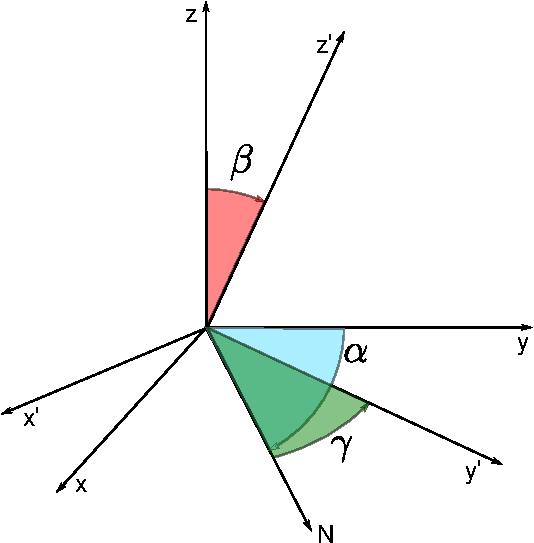
\includegraphics[width = 0.5\textwidth]{figs/eulerAnglesDefinition.pdf}
  \caption{Definition of the Euler angles $\alpha,\beta$ and $\gamma$ used to transform from the coordinate
           frame spanned by $x,y,z$ to the frame spanned by $x^\prime,y^\prime,z^\prime$. The intersection
           between $xy$- and $x^\prime y^\prime $-plane is denoted by $N$. Note that the sign of all angles
           are defined via the plane they are located in ($xy$- or $zy$-plane).}
  \label{fig:EulerAnglesDefinition}
\end{figure}

Molecular orbitals are expressed in terms of so-called real-spherical harmonics $S_{lm}$ (angular momentum $l$
and orientation $m$) which are linear combinations of their complex counter parts $Y_{lm}$, the eigenfunctions
of the angular momentum operator in $z$ direction $\hat{l}_z$. Since the $Y_{lm}$ are degenerate in $m$ for a
radial symmetric Hamiltonian, we are free to construct the linear combinations $S_{lm}$ without changing their
eigenvalue with respect to the Hamiltonian. Thus, the set of functions $S_{lm}$ may be constructed from the
functions $Y_{lm}$ and it may be shown that they represent a complete basis set for a given $l$\cite{Blanco1997}.

The rotation around the $z$-axis may be expressed in terms of the complex-spherical harmonics. In this basis
the rotation matrix associated to $\hat{R}_z$ is diagonal. Thus, the rotation around the $z$ axis may be
expressed in the basis of the real spherical harmonics as
\begin{align}
  \pmb{X}_l(\alpha) = \pmb{C}_l^\dagger \mathrm{Diag}(e^{im\alpha,m=-l,...l})\pmb{C}_l,
\end{align}
where $\mathrm{Diag}(e^{im\alpha,m=-l,...l})$ is the rotation matrix in basis of the complex-spherical harmonics,
and $\pmb{C}_l$ is the (unitary) transformation matrix between real and complex-spherical harmonics.

The matrix representation $\pmb{\Delta}_l(\alpha,\beta,\gamma)$ of the rotation of a set of functions expressed in
the basis of $S_{lm}$ by $\hat{R}$ is then given as
\begin{align}
  \pmb{\Delta}_l(\alpha,\beta,\gamma) = \pmb{X}_l(\alpha) \pmb{D}_l(\beta) \pmb{X}_l(\gamma).
  \label{eq:GeneralRotationWigner}
\end{align}
Here, $\pmb{D}_l(\beta)$ denotes the matrix of the rotation $\hat{R}_y(\beta)$ in the basis of $S_{lm}$
\cite{Blanco1997}.

In 2007 Pinchon and Hoggan\cite{Pinchon2007}, showed that $\pmb{D}_l(\beta)$ may be obtained by first exchanging the
coordinates of $y$ and $z$, rotating around $z$ and then exchanging the coordinates again. If we denote the matrix
for the exchange of $y$ and $z$ in the basis of $S_{lm}$ as $\pmb{J}_l$, we may write
\begin{align}
  \pmb{D}_l(\beta) = \pmb{J}_l \pmb{X}_l(\beta) \pmb{J}_l.
\end{align}
With this, Eq.~(\ref{eq:GeneralRotationWigner}) becomes
\begin{align}
  \pmb{\Delta}_l(\alpha,\beta,\gamma) = \pmb{X}_l(\alpha) \pmb{J}_l \pmb{X}_l(\beta) \pmb{J}_l \pmb{X}_l(\gamma).
  \label{eq:SphericalHarmonicsRotation}
\end{align}
In contrast to previous works\cite{Ivanic1996,Blanco1997}, only the exchange matrices
$\pmb{J}_l$ have to be calculated using recursive schemes, since an explicit expression for the matrix
$\pmb{X}_l(\alpha)$ is known.
It has only non-zero elements on its diagonal and anti-diagonal. For $l=2$, $\pmb{X}_2(\alpha)$ is given by
\begin{align}
  \pmb{X}_2(\alpha) = \begin{pmatrix}
                      \cos(2\alpha) & 0            & 0 & 0            & \sin(2\alpha) \\
                      0             & \cos(\alpha) & 0 & \sin(\alpha) & 0 \\
                      0             & 0            & 1 & 0            & 0 \\
                      0             & -\sin(\alpha)& 0 & \cos(\alpha) & 0 \\
                      -\sin(2\alpha)& 0            & 0 & 0            & \cos(2\alpha)
                      \end{pmatrix}.
\end{align}

The recurrence expressions for $\pmb{J}_l$ for $l \leq 1$ are given by
\begin{align}
  \begin{split}
    \pmb{G}^l_x \pmb{J}_l &= \pmb{J}_{l+1}\pmb{G}^l_x\\
    \pmb{G}^l_z \pmb{J}_l &= \pmb{J}_{l+1}\pmb{G}^l_y\\
    \pmb{G}^l_y \pmb{J}_l &= \pmb{J}_{l+1}\pmb{G}^l_z,
  \end{split}
  \label{eq:GauntTransformation}
\end{align}
where $\pmb{G}^l_x$, $\pmb{G}^l_y$ and $\pmb{G}^l_z$ are the matrices of the so-called Gaunt coefficients. Their
non-zero elements are given by
\begin{align}
  \begin{split}
    \kappa_l &= \frac{1}{2\sqrt{(2l+1)(2l+3)}},\\
    \left(\pmb{G}^l_x\right)_{2+k,k} = \left(\pmb{G}^l_x\right)_{2l+2-k,2l+2-k}&
    = \left(\pmb{G}^l_y\right)_{2l+2-k,k} = -\left(\pmb{G}^l_y\right)_{2+k,2l+2-k}\\
    &= \kappa_l\sqrt{k(k+1)},
    ~~~1\leq k \leq l-1,\\
    \left(\pmb{G}^l_x\right)_{k,k} = \left(\pmb{G}^l_x\right)_{2l+4-k,2l+2-k}
    &= \left(\pmb{G}^l_y\right)_{k,2l+2-k} = -\left(\pmb{G}^l_y\right)_{2l+4-k,k}\\
    &=-\kappa_l \sqrt{(2l+2-k)(2l+3-k},
    ~~~1\leq k \leq l,\\
    \left(\pmb{G}^l_x\right)_{l+2,l+2} = \left(\pmb{G}^l_y\right)_{l+2,l} &= \kappa_l \sqrt{2l(l+1)},\\
    \left(\pmb{G}^l_x\right)_{l+3,l+1} = \left(\pmb{G}^l_y\right)_{l+1,l+1} &= -\kappa_l \sqrt{2(l+1)(l+2)},\\
    \left(\pmb{G}^l_z\right)_{k+1,k} &= 2\kappa_l \sqrt{k(2l+2-k)},~~~ 1 \leq k \leq 2l+1.
  \end{split}
\end{align}
In order to calculate the entries of $\pmb{J}_l$, only the diagonal, non-zero block ($\hat{\pmb{G}}^l_z$)
of $\pmb{G}^l_z$ and $\pmb{G}^l_y$ are needed. $\pmb{J}_{l+1}$ may then be written as
\begin{align}
  \pmb{J}_{l+1} = \begin{pmatrix}
                    0      & ~ & 0 \\
                    \vdots &  \pmb{G}^l_y \pmb{J}_{l} \left(\hat{\pmb{G}}^l_z\right)^{-1} & \vdots\\
                    0      & ~ & 2^{-l}
                  \end{pmatrix},
  \label{eq:Recurrence}
\end{align}
where the central block of columns (all columns except the first and last one) are given by
$\pmb{G}^l_y \pmb{J}_{l} \left(\hat{\pmb{G}}^l_z\right)^{-1}$. The missing rows of the first and last column
can be constructed from the requirement of the matrix $\pmb{J}_{l}$ to be symmetric.

The matrices $\pmb{J}_{l}$ for $l=1$ and $l=0$ are given by
\begin{align}
  \pmb{J}_{0} = \begin{pmatrix}
                    1
                  \end{pmatrix},
\end{align}
and
\begin{align}
  \pmb{J}_{1} = \begin{pmatrix}
                  0 & -1 & 0 \\
                  -1&  0 & 0 \\
                  0 &  0 & 1
                \end{pmatrix}.
\end{align}
All other matrices for $l > 1$ may be computed using Eq.~(\ref{eq:Recurrence}).

\subsection{Copying and Pasting Molecular Orbitals}

Consider two molecules $A$ and $B$ which are identical up to translation and rotation. The molecular-orbitals set
$\{\psi^{A}_i\}$ of molecule $A$ is known and expressed in a set of spherical, atom-centered basis functions with
coefficients $\pmb{C}^A$. Our goal is to obtain the coefficients $\pmb{C}^B$ that correspond to the set
$\{\psi^{B}_i\}$ by translating and rotating the set $\{\psi^{A}_i\}$. Since the atoms of both molecules are the same,
their exists a one to one mapping of basis function shells. Thus, the translational part is trivially taken care of,
i.e. if the molecules are not rotated with respect to each other the coefficient matrices $\pmb{C}^A$ and
$\pmb{C}^B$ will be identical. In case of rotation, we first calculate the Euler angles ($\alpha_A$, $\beta_A$,
$\gamma_A$) for the rotation of the Cartesian frame to the internal frame of $A$. We can then rotate the
$\{\psi^{A}_i\}$ to the Cartesian frame by rotating the coefficient matrix in a shell-wise manner with the
transformation matrix $\pmb{\Delta}_l$ from Eq.~(\ref{eq:SphericalHarmonicsRotation}),
\begin{align}
  \left(\pmb{C}^\mathrm{Cart}\right)_{\mu_l} = \pmb{\Delta}_l(-\gamma_A,-\beta_A,-\alpha_A)\left(\pmb{C}^A\right)_{\mu_l},
\end{align}
where the subscript ${\mu_l}$ denotes the basis-function block associated to the shell $\mu_l$ with
angular momentum $l$.

The orbitals can then be rotated from the Cartesian frame to the internal frame of $B$ with the Euler angles
for the rotation of the Cartesian to the internal frame $B$ ($\alpha_B$, $\beta_B$, $\gamma_B$) as
\begin{align}
  \left(\pmb{C}^B\right)_{\mu_l} = \pmb{\Delta}_l(\alpha_B,\beta_B,\gamma_B)\left(\pmb{C}^\mathrm{Cart}\right)_{\mu_l}.
\end{align}

\subsection{Internal Frame Construction}

Each molecule is represented by the coordinates of its atoms $\{\pmb{a}_i\}$ in the Cartesian frame.
The internal $x$-axis $\pmb{e}_x$ is constructed as
\begin{align}
  \pmb{e}_x = \frac{(\pmb{a}_1-\pmb{a}_0)}{|\pmb{a}_1-\pmb{a}_0|},
\end{align}
the $y$-axis is constructed as
\begin{align}
  \pmb{e}_y = \frac{\pmb{t}_y}{|\pmb{t}_y|},
\end{align}
where $\pmb{t}_y$ is the orthogonalized difference vector between the coordinates of $1$ and $2$
which is defined with the difference vector $\pmb{d}_{21} = \pmb{a}_2-\pmb{a}_1$ as
\begin{align}
  \pmb{t}_y = \pmb{d}_{21}-\pmb{e}_x\pmb{e}_x^\dagger\pmb{d}_{21}.
\end{align}
The $z$-axis that belongs to a right-handed coordinate system can then be obtained as
\begin{align}
  \pmb{e}_z = \pmb{e}_x \times \pmb{e}_y.
\end{align}
Note that some special cases for highly symmetrical molecules need to be handled:
(i)   If the molecule consists of only one atom, the Cartesian frame is used as the internal frame.
(ii)  If the molecule consists of only two atoms, the vector $\pmb{d}_{21}$ is chosen to be the Cartesian
      $x$-axis if $\pmb{e}_x$ does not depend linearly on it. Otherwise the $y$-axis is chosen.
(iii) If the vector $\pmb{d}_{21}$ is linear depended on $\pmb{e}_x$, the difference vector $\pmb{d}_{31}$ is
      chosen for the construction of $\pmb{e}_y$. This is repeated until $\pmb{e}_y$ can be constructed. If there
      is no linear independent difference vector, the approach given in (ii) is used.

\section{Molecular Cavity and Surface Construction\label{sec:MolcSurface}}
This chapter describes the implementation of the molecular surface and cavity construction as
proposed by B. Delley\cite{Delley2006}.

\subsection{Molecular Surface Model}
Delley used for the molecular surface the zero-isosurface of a ball-and-stick-like
model function $F(\pmb{r})$ that varies continuously with the position $\pmb{r}_i$
and radii $R_i$ of the atoms. $F(\pmb{r})$ is given by
\begin{align}
  F(\pmb{r}) = 1+\sum_i f\left(\frac{(\pmb{r}-\pmb{r}_i)^2-R_i^2}{2R_sR_i} \right)
                +\sum_{i\neq j} f\left( \frac{\left[\pmb{r}-\pmb{r}_z(ij)\right]^2-R_z^2(ij)}{2R_s \max(R_z, 1.0~\text{au})} \right),
  \label{eq:delleyModelFunction}
\end{align}
where the auxiliary function $f(x)$ is given by
\begin{align}
  f(x) = -\exp(-\alpha x) + ax + b x^2.
\end{align}
The parameters $a$ and $b$ are obtained from the boundary conditions
$f(4/\alpha) = 0$ and $f^\prime(4/\alpha) = 0$. The radius of the solvent
probe is given by $R_s$. The parameter $R_z(ij)$ is the radius of a cylinder
that touches the spheres $i$ and $j$ as well as the solvent probe with radius
$R_s$, which in turn touches both spheres $i$ and $j$. It is given
with $S_i = R_i + R_s$ and $d_{ij} = |\pmb{r}_i-\pmb{r}_j|$ by
\begin{align}
  R_z(ij) = \sqrt{S_i^2 - \left( \frac{S_i^2+d_{ij}^2-S_j^2}{2d_{ij}} \right)^2}-R_s.
\end{align}
The parameter $\pmb{r}_z(ij)$ is the point of the orthogonal projection of the
point $\pmb{r}$ onto the bond between the spheres $i$ and $j$. If this projection
does not lie between spheres $i$ and $j$, $\pmb{r}_z(ij)$ is defined as the respective
bond end $\pmb{r}_i$ or $\pmb{r}_j$.
The bond part of the model (third term in Eq.~[\ref{eq:delleyModelFunction})] is restricted
to pairs $ij$ for which $d_{ij} \leq S_i+S_j$.


The model function $F(\pmb{r})$ can be understood as placing a function
$1-\exp\left[-\alpha (r-R)\right]$ on every atom and on every bond of the molecule.
Thus, $F(\pmb{r})$ will have large negative values within the molecule, a value of
$0$ at the molecular surface and a value of $1$ far outside the molecule. The parameter
$\alpha$ controls how sharp the superposition of functions from different spheres or
cylinders is. It is typically set to $\alpha = 50.0$. For small values of $\alpha$ the
surface may become blurred.

\subsection{Molecular Surface Discretization}
For the application of continuum solvation models\cite{Tomasi2005} it is necessary to
discretize the surface into small areas with one representative point each, so-called tesserae.
This is achieved by atom-wise projection of spherical integration grids to the molecular
surface as shown in Fig.~\ref{fig:delleySurfaceConstruction}(a). The normal vectors $\pmb{n}_p$
at the position of the grid point $\pmb{r}_p$, which are needed for some continuum models, are obtained as
normalized vectors with the direction of $\left.\nabla F(\pmb{r})\right|_{\pmb{r}=\pmb{r}_p}$.
In \textsc{Serenity} the standard spherical grid point distributions by Lebedev and Laikov are used.
\begin{figure}
	\centering
	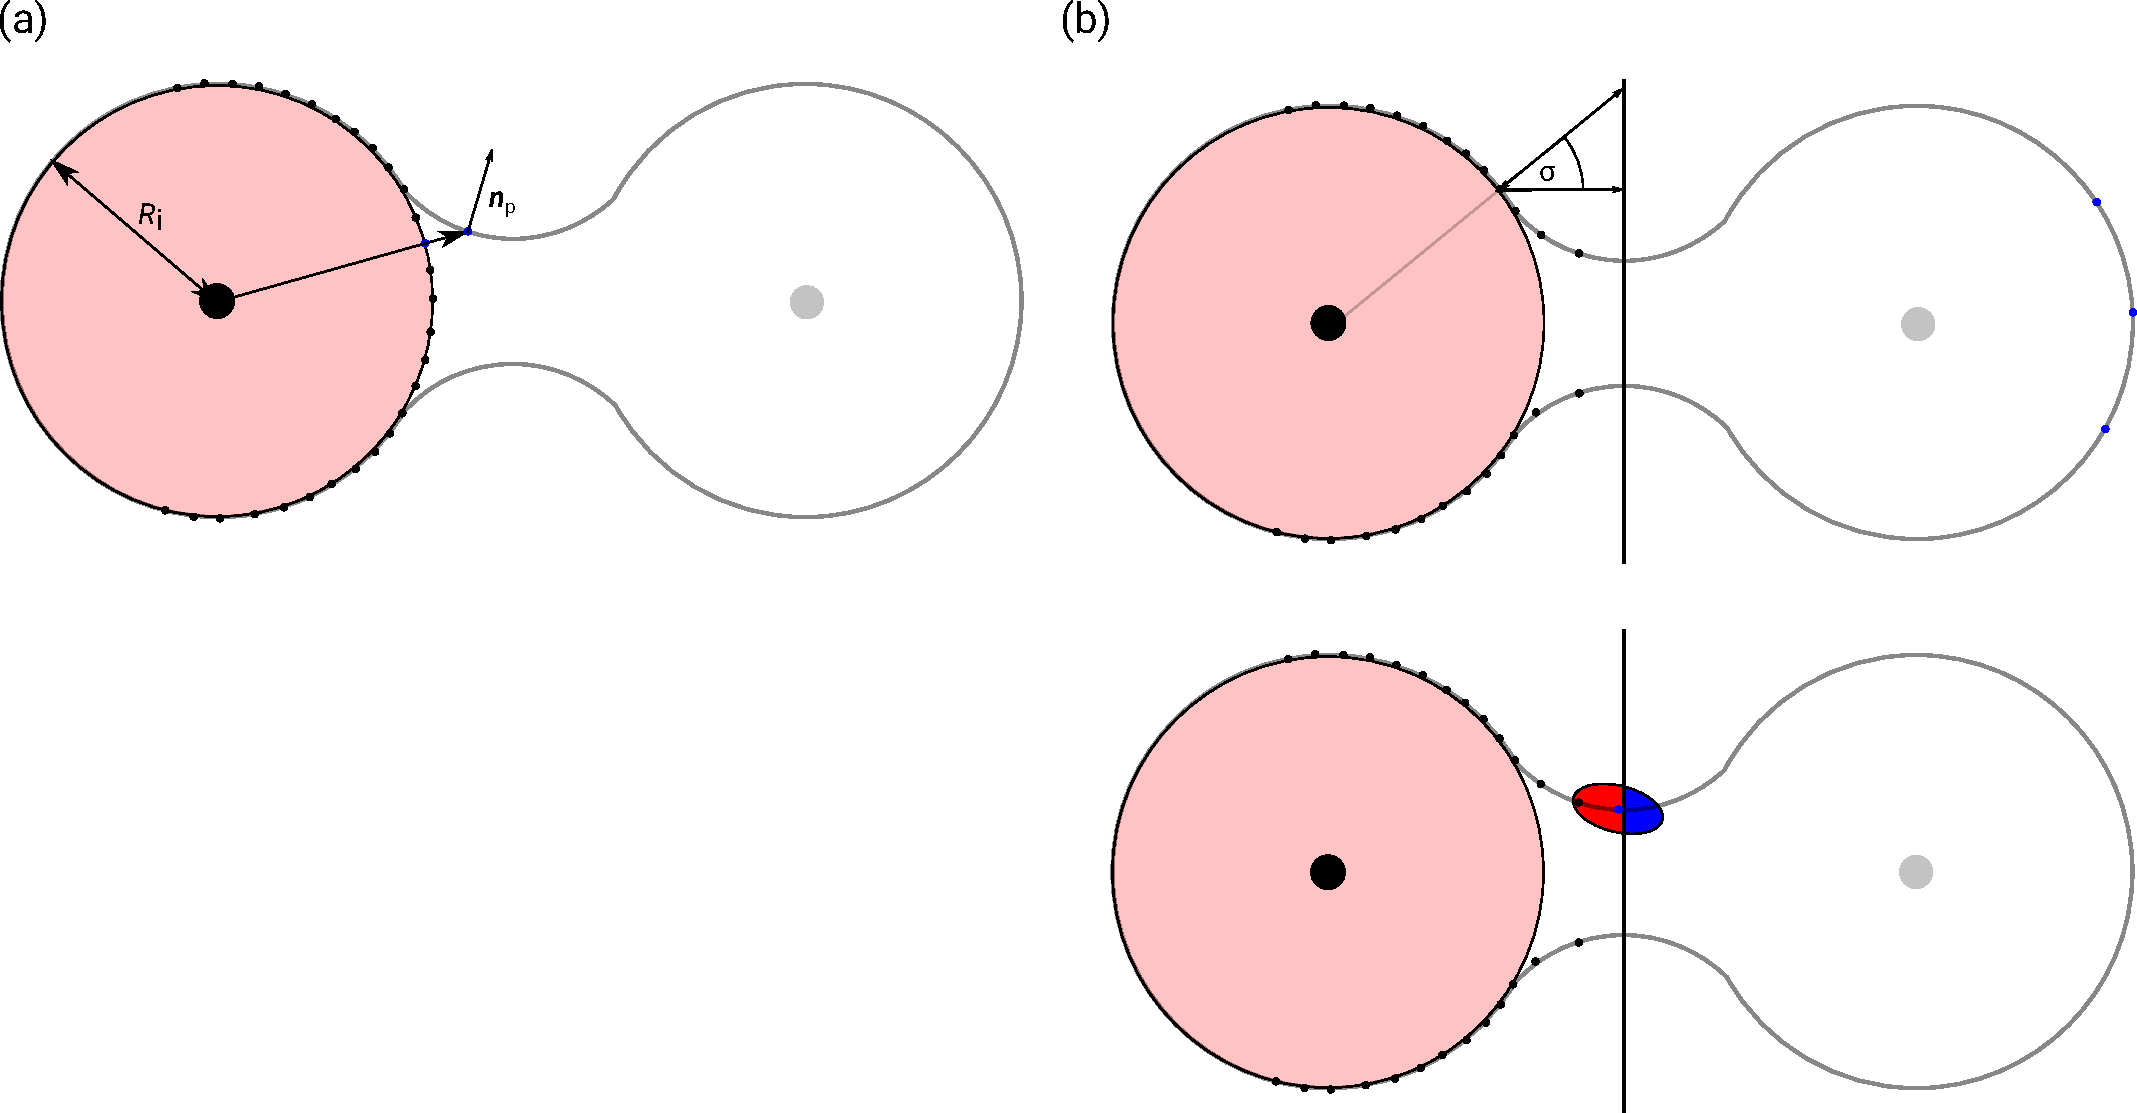
\includegraphics[width=0.95\textwidth]{figs/delleyFigure.pdf}
	\caption{Schematic of the surface mesh construction for a diatomic molecule.
			 (a) Projection of the spherical grid points to the molecular surface, and
			     construction of the normal vector $\pmb{n}_p$.
			 (b) Area scaling and cutting for grid points on the bond part of the molecular
			     surface.}
	\label{fig:delleySurfaceConstruction}
\end{figure}

The initial weights or areas $A_p^\prime$ associated to each point are calculated as
\begin{align}
	A_p^\prime = 4.0\pi A_{i,p}^{u}|\pmb{r}_p-\pmb{r}_i|^2,
\end{align}
where $A_{i,p}^{u}$ is the weight of the grid point on the unit sphere surrounding sphere $i$.
These weights are then scaled by the skew projection on the bond plane as $A_p^s = \sin(\sigma) A_p^\prime$
(see Fig.~\ref{fig:delleySurfaceConstruction}(b)) if they fall on the bond part of the surface
($\pmb{r}_z(ij) \neq \pmb{r}_i$ and $\pmb{r}_z(ij) \neq \pmb{r}_j$) and a bond between the spheres exists.
We then define planes $P(ij)$ orthogonal to each bond $ij$ (plane normal vectors
$\pmb{n}_\mathrm{bond} = \frac{\pmb{r}_i-\pmb{r}_j}{|\pmb{r}_i-\pmb{r}_j|}$) which contain the points
$\pmb{c}_\mathrm{bond} = \frac{R_i}{R_i+R_j} \pmb{r}_i +\frac{R_j}{R_i+R_j} \pmb{r}_j$, which
are the weighted centers of the bonds. We then consider each point on a bond to be an ellipse with
radial vectors $\pmb{r}_1$ and $\pmb{r}_2$ ($\pmb{r}_1^\dagger\pmb{r}_2 = 0$) given as
\begin{align}
	\pmb{r} = \pmb{r}_1 \cos(t) + \pmb{r}_2 \sin(t),~t\in [0,2\pi].
\end{align}

The ellipse construction is illustrated in Fig.~\ref{fig:ellipseConstruction}.
The direction of $\pmb{r}_1$ is obtained as the direction $\pmb{d}_s$ of the intersection between
the plane on the original sphere (its normal vector is equal to the vector $\pmb{n}_\mathrm{pro}$
used for the projection of the point to the surface) and the plane containing
the projected point, described by the normal vector $\pmb{n}_p$. The direction of $\pmb{r}_2$ is obtained by
requiring that $\pmb{r}_2$ is orthogonal to $\pmb{r}_1$ and $\pmb{n}_p$.

The length of the radial vectors is calculated by projecting a point on the circle
on the initial sphere to the plane on the molecular surface as shown in Fig.~\ref{fig:ellipseConstruction}
for $\pmb{r}_1$. The same procedure is applied for $\pmb{r}_2$. The vectors are then scaled such that
the ellipse contains the area $A_p^s$.


\begin{figure}[H]
	\centering
	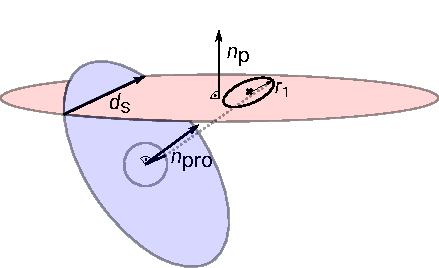
\includegraphics[width=0.8\textwidth]{figs/ellipseConstruction.pdf}
	\caption{Illustration of the ellipse construction for the area scaling.
	         The direction of the intersection between the plane on the initial sphere ($blue$)
	         and the plane on the molecular surface $red$ is denoted with $\pmb{d}_s$.
	         The vector $\pmb{r}_1$ is obtained by going from the center of the circle on the
	         initial sphere in direction of $\pmb{d}_s$ according to the area of the circle.
	         Then a line is constructed containing this point with direction $\pmb{n}_\mathrm{pro}$,
	         and the intersection with the $red$ plane is calculated. The same is done for $\pmb{r}_2$.
	         Both vectors are then scaled such that the ellipse has the desired area.}
	\label{fig:ellipseConstruction}
\end{figure}

If an ellipse is cut by a plane $P(ij)$ [see Fig.~\ref{fig:delleySurfaceConstruction}(b)], the area and the center
of gravity $\pmb{r}_{p,\mathrm{grav}}$ not hidden by the plane from the perspective of the owning atom is calculated.
If the ellipse is completely hidden by the plane, the point is dropped.
The center of gravity is projected back to the molecular surface along the direction
$\pmb{r}_{p,\mathrm{grav}}-\pmb{r}_i$ and a new ellipse is constructed. This procedure is repeated for all $j$ bonding
with $i$. This construction ensures that all points remain on the bond side of their initial atoms.

\section{Cholesky Decomposition}

The Cholesky decomposition is a mathematical procedure that enables to speed up many applications in theoretical chemistry. It allows to decompose a hermitian, positive (semi-)definite matrix $M$ into a lower triangular matrix $L$ and its transposed

\begin{equation}
M=LL^T.
\end{equation}

It can for example be applied to decompose the two-electron four-center integral matrix  into three index objects

\begin{equation}\label{CDMatrix}
\langle \mu \nu | \lambda \sigma \rangle = \sum_P^M \langle \mu \nu | P \rangle \langle P | \lambda \sigma \rangle = \sum_P^M L^P_{\mu\nu} L^P_{\lambda\sigma} ,
\end{equation}

where the greek letters are indices of the basis functions $\phi_\mu$ and the counting index $P$ refers to which Cholesky vector is used. This Cholesky vector is equivalent to the $P$th column in the matrix $L$. Consequently, $M$ is the number of Columns in $L$ or the number of Cholesky vectors. The mapping of the column or row indices of the original matrix to the indices of the Choleky vectors is called the Cholesky basis.\\

To see why this decomposition is useful in speeding up calculations, one can compare it to the well established resolution of the identity (RI) approach. Here, the basis is projected to the space of a prefitted auxiliary basis so that it seems that the identity of the auxiliary basis was inserted into the original expression
\begin{equation}\label{RIFull}
\langle \mu \nu | \lambda \sigma \rangle \approx \sum_{P,Q} \langle \mu \nu | P \rangle \langle P | Q \rangle^{-1} \langle Q | \lambda \sigma \rangle .
\end{equation} 

If simplified using

\begin{equation}
B_{\mu \nu,Q} = \sum_{P} \langle \mu \nu | P \rangle \langle P | Q \rangle^{-1/2},
\end{equation}

the equation becomes 

\begin{equation}
\langle \mu \nu | \lambda \sigma \rangle \approx \sum_{Q} B_{\mu \nu,Q} B_{\lambda \sigma,Q}.
\end{equation} 

Comparing this result to Eq.~\ref{CDMatrix} it becomes evident that they are equivalent and can be evaluated with similar efficiency. However, one has to keep in mind that, in general, the basis obtained in all Cholesky procedures is larger than the prefitted auxiliary basis sets used in the RI approach. As a result, Cholesky based calculations will always be slower than comparable RI calculations if available.\\

The advantage of Cholesky Decomposition compared to RI is that, as shown in the following sections, it offers error control for all elements in the matrix that is decomposed. This is in contrast to the RI approach, where the auxiliary basis is fitted to reproduce on particular metric (like for example the Coulomb energy contribution), but a reconstruction of the original matrix as in Eq.~\ref{RIFull} will contain significant errors.


\subsection{The Decomposition Algorithm}

A basic algorithm to perform the Cholesky decomposition is given below (Algorithm 1). It features pivoting, which means that no full decomposition is performed but that the decomposition is stopped once a certain accuracy in each matrix element (given by the decomposition threshold $\delta$ ) is reached. The drawback of this algorithm is that it requires the original matrix $M$ to be stored in memory in its entirety. This normally is no problem but the full two-electron four-center integrals can quickly take up more memory than available in modern clusters.

\begin{figure}[h!]
	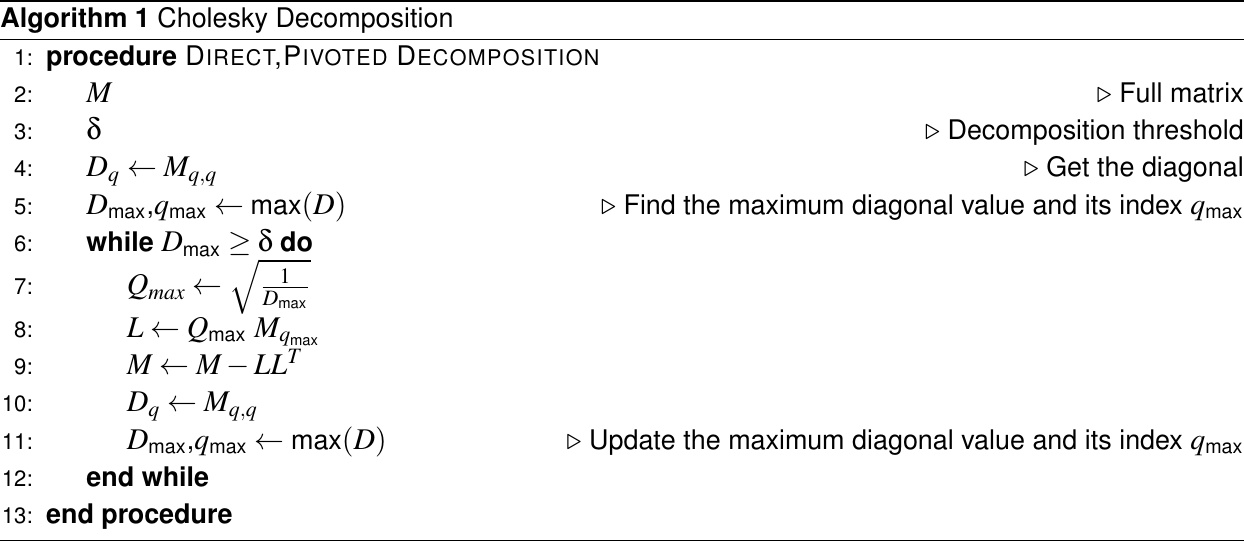
\includegraphics[width=\textwidth]{cholesky/algorithm1.png}
\end{figure}

To circumvent this problem, a memory efficient algorithm is implemented in \textsc{Serenity} (Algorithm 2). This algorithm firstly analyzes the diagonal to find the columns that have the potential to contribute to the Cholesky vectors and summarizes the corresponding indices in the reduced set $\mathcal{R}$. Then, the most significant elements in $\mathcal{R}$ are determined and summarized in the qualified set $\mathcal{Q}$. In general, this set is obtained by checking if the diagonal element is larger than $D_\text{min}$ but, in practice, the size of $\mathcal{Q}$ is also limited to a smaller number of elements to ensure memory and general efficiency (this avoids the calculation and later subtraction of too many elements that ultimately do not contribute to the Cholesky vectors, due to linear dependencies in $\mathcal{Q}$). As a result, in each iteration only the subset of integrals spanned by $\mathcal{Q}$ and $\mathcal{R}$ has to be calculated. Furthermore, the quite expensive subtraction step only has to be performed on that subset of integrals during each iteration. This also means that, in the end, the Choleksy vectors are calculated only in the subspace of $\mathcal{R}$ and have to be mapped to the corresponding indices in the complete set $\mathcal{S}$. Another important feature of this algorithm is checking for numerical errors. These can lead to small negative entries in the diagonal, which in turn can lead to errors in the calculation of $Q_{\text{max}}$. The last feature worth mentioning is the pre-screening of the qualified set $\mathcal{Q}$ for all elements that will actually contribute to the Cholesky vectors. This step exploits the fact that a decomposition of a matrix spanned by $\mathcal{Q}$ and $\mathcal{R}$ will yield the same contributing indices as the decomposition of the matrix spanned by $\mathcal{Q}$ and $\mathcal{Q}$. Since the dimension of $\mathcal{Q}$ is significantly lower than that of $\mathcal{R}$, the overhead created by additional decomposition step is negligible compared to the computational savings in the following steps.

\begin{figure}
	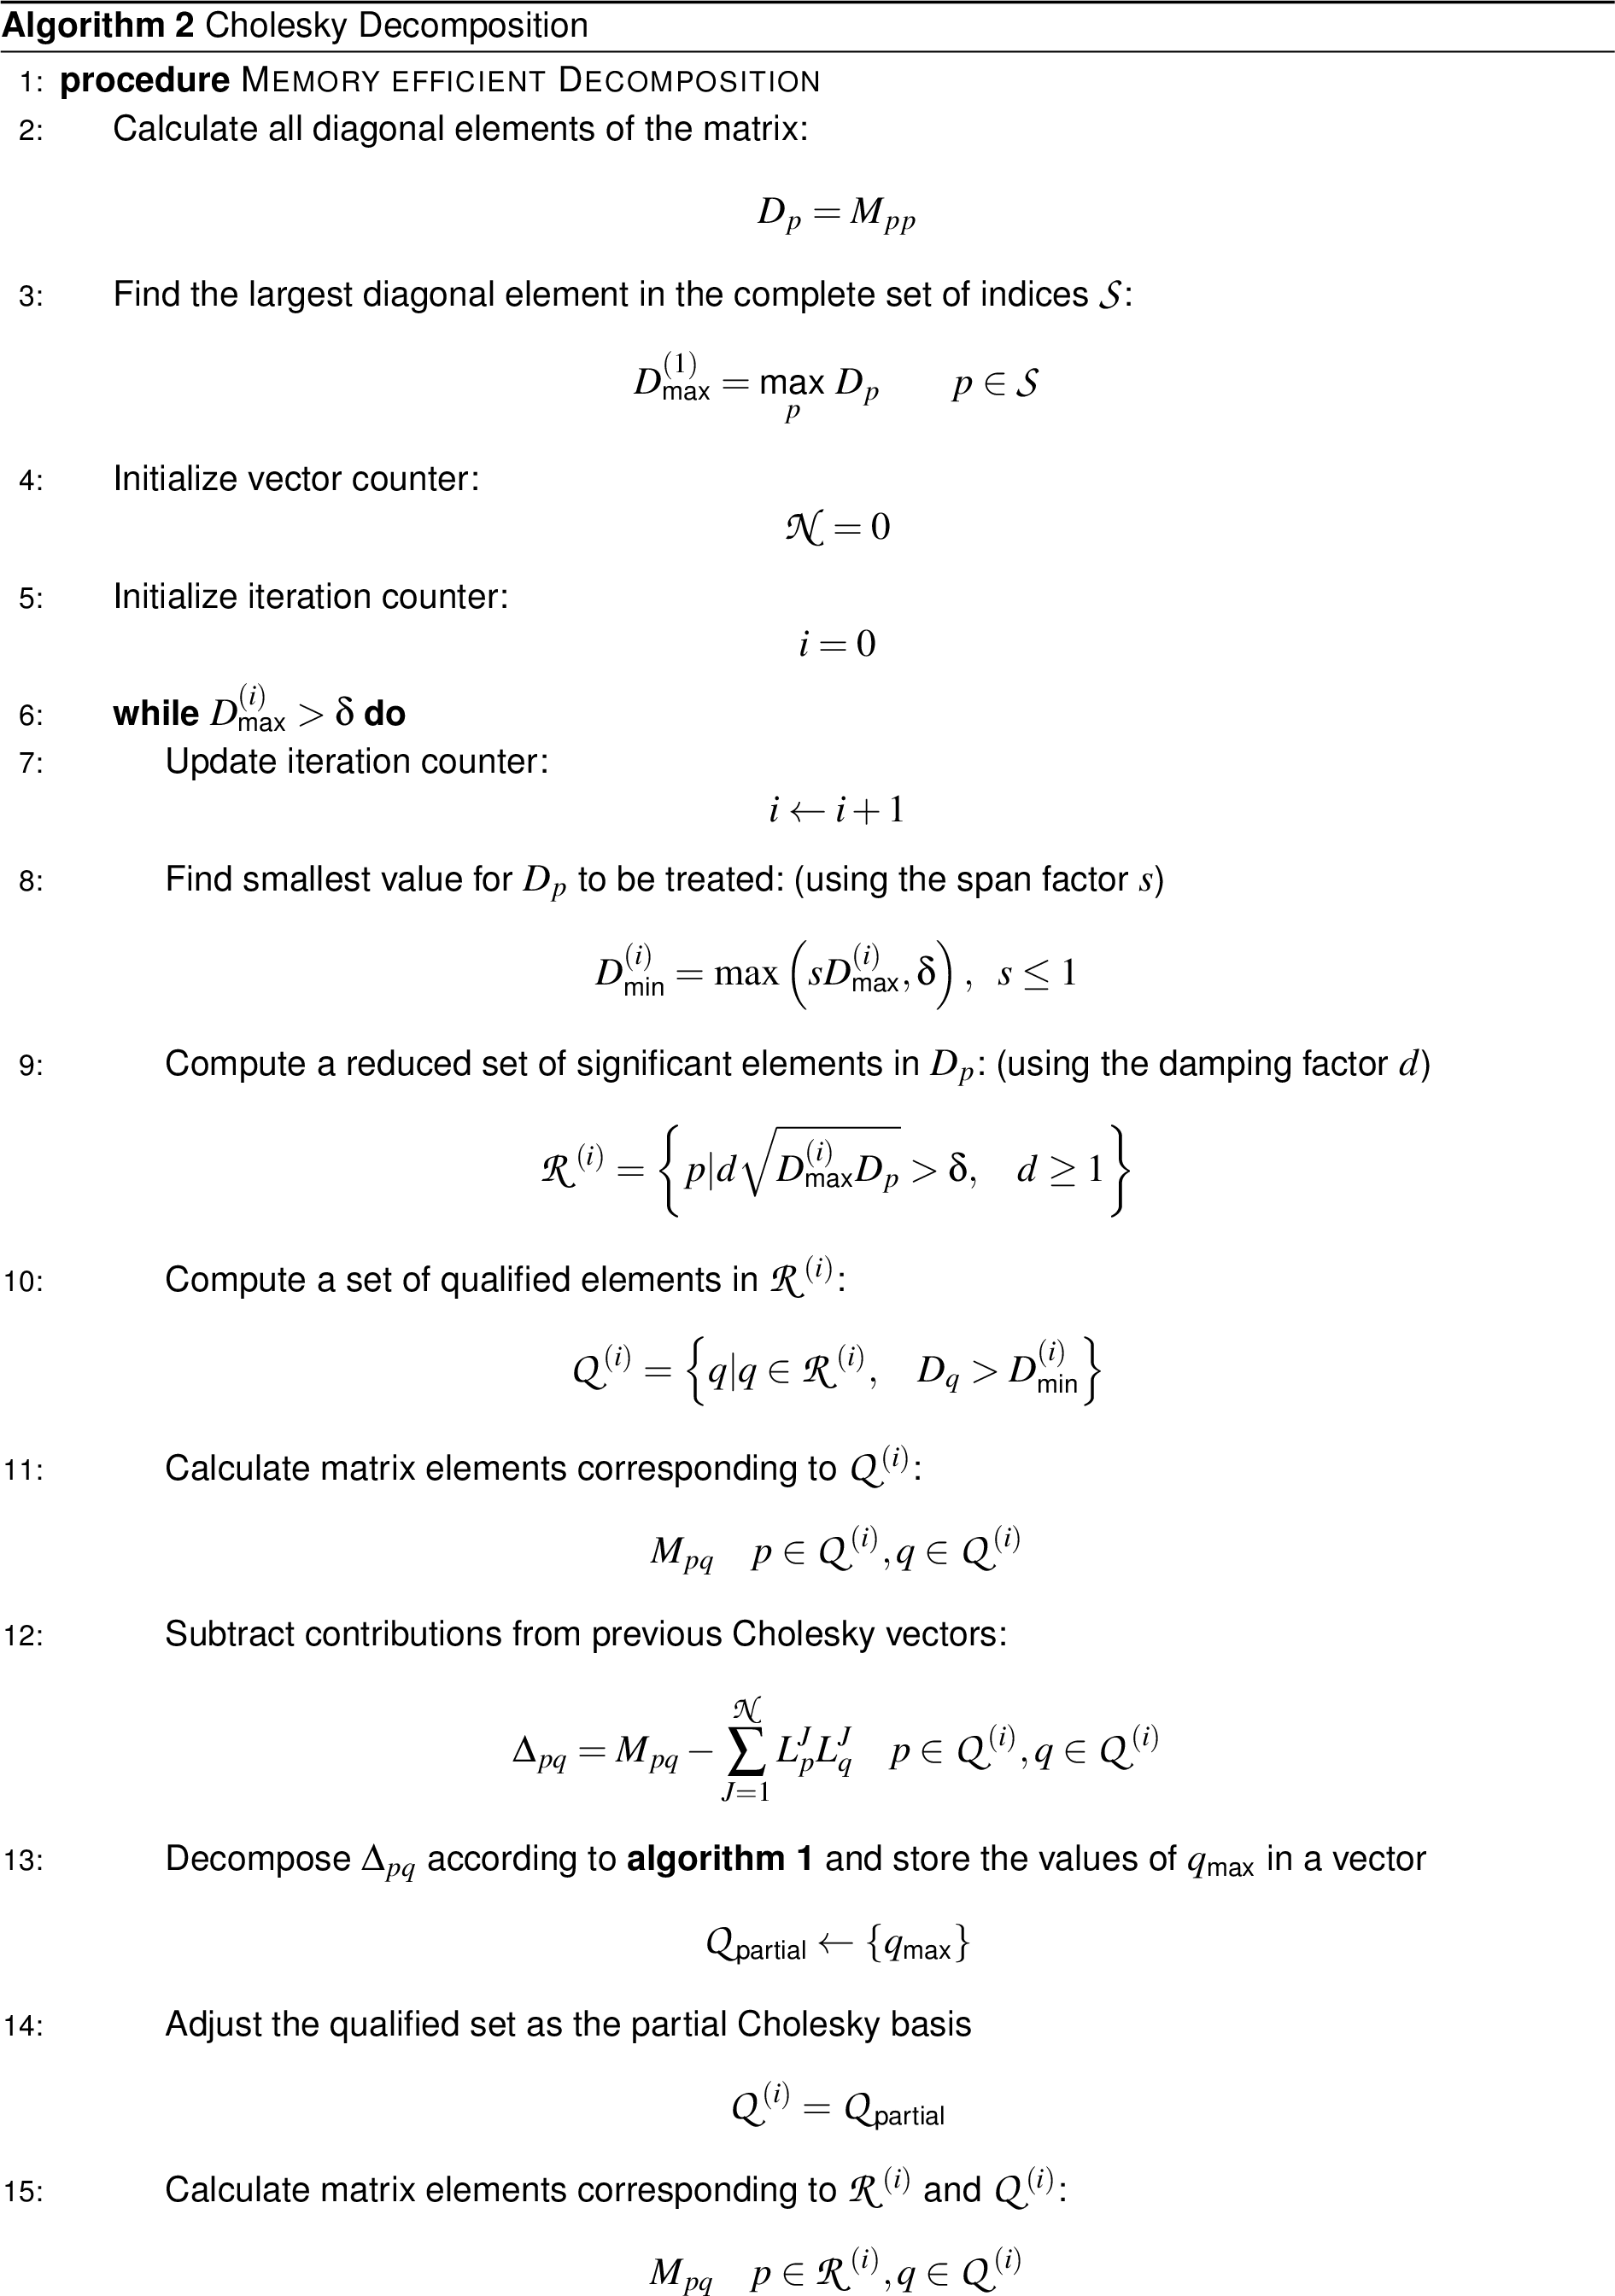
\includegraphics[width=\textwidth]{cholesky/algorithm2_1.png}
\end{figure}

\begin{figure}
	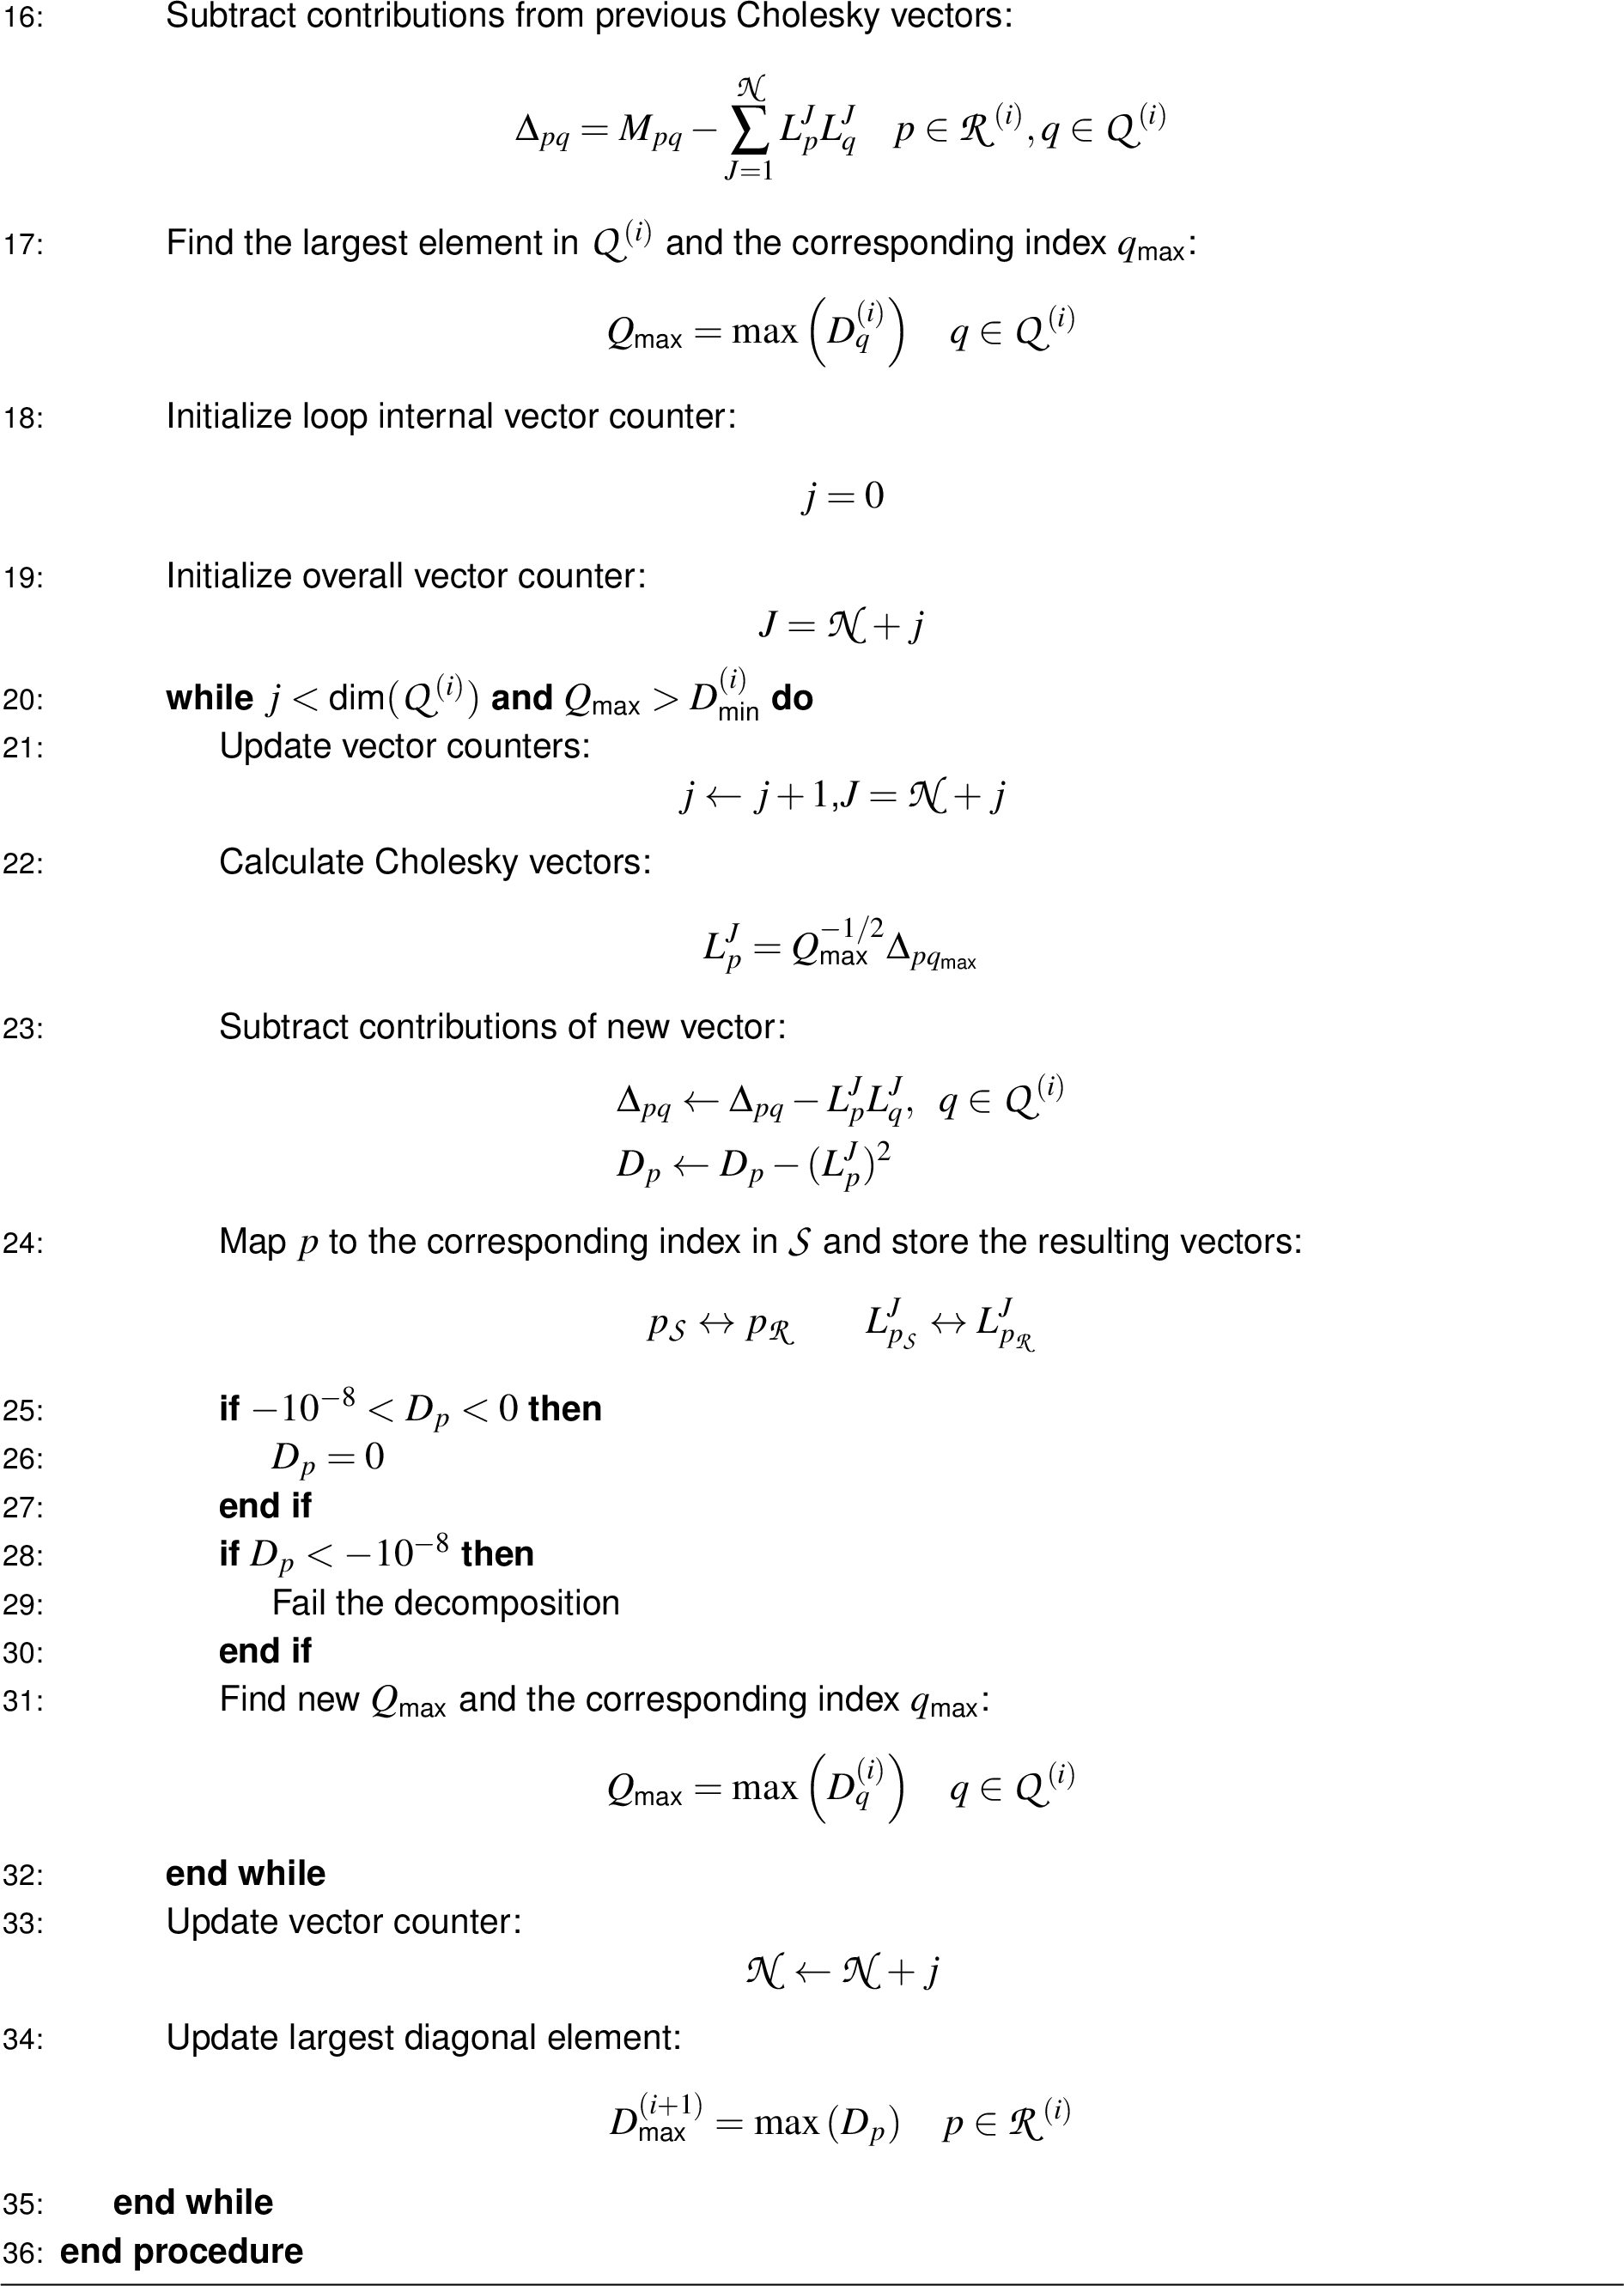
\includegraphics[width=\textwidth]{cholesky/algorithm2_2.png}
\end{figure}



\subsection{The Atomic Cholesky Decomposition}

One major problem of the generic Cholesky decomposition approach is that it needs to decompose the complete two-electron four-center integral matrix. This is easily feasible for small systems, but at the latest when it is no longer possible to hold the full matrix in memory it becomes a time-determining step. In order to remove this unfavorable behavior, an additional approximation can be introduced. Instead of enforcing a strict error control in all integrals, the atomic Cholesky decomposition (ACD) only enforces this strict control in the integrals where all four basis functions are centered at the same point. This is done by decomposing the two-electron four-center integrals of the isolated atom types
\begin{equation}\label{ACDMAtrix}
\langle \mu \nu | \lambda \sigma \rangle \approx \sum_P^M L^P_{\mu\nu} L^P_{\lambda \sigma} ,
\end{equation}
where $P$ is spans the subspace of all linearly independent basis function products $\phi_\mu \phi_\nu$. This identification allows to generate a new auxiliary basis set, where the basis functions are chosen as $$\phi_P = \phi_\mu \phi_\nu .$$ 
As a result, if we use the obtained auxiliary ACD basis in a way similar to the RI approach
\begin{equation}\label{ACDFormalism}
\langle \mu \nu | \lambda \sigma \rangle \approx \sum_{P,Q} \langle \mu \nu | P \rangle \langle P | Q \rangle^{-1} \langle Q | \lambda \sigma \rangle ,
\end{equation} 
one still retains strict error control for the integrals centered only at one atom. For all other elements residing on more than one center an error minimization is retained. The big advantage of this method is that the generation of the auxiliary basis set does not scale with the size of the system itself but only with the number of different atom types and the size of the basis set used, enabling it to generate these auxiliary basis sets on the fly for each calculation with minimal overhead.

\subsection{The Atomic Compact Cholesky Basis}

The big problem inherent to the ACD approach are the basis-function products used as the new basis functions, as these are contracted Gaussian-type functions 
\begin{equation}
\phi_\mu^c = \sum_i^{n_i} c_i \phi_{i,\mu}^p 
\end{equation}
and their products are given as
\begin{equation}
\phi_P = \phi_\mu^c \phi_\nu^c = \sum_i^{n_i} \sum_j^{n_j} c_i c_j \phi_{i,\mu}^p \phi_{j,\nu}^p .
\end{equation}
It can be easily seen that the number of primitive basis functions for one contracted basis function scales with $\mathcal{O}(n_i^2)$, which makes the computation of the integrals very expensive or even impossible with the corresponding libraries used in \textit{Serenity}. 
The atomic compact Cholesky decomposition (ACCD) makes use of the fact that linear dependencies within this massive space of primitive basis functions will occur again. They can be removed by setting up the two-electron two-center integral matrix of the primitive basis functions in one contracted basis function, and decompose it as
\begin{equation}
\langle	\mu^p | \nu^p \rangle \approx \sum_P^M L^P_{\mu^p} L^P_{\nu^p} ,
\end{equation}
allowing to remove primitive basis functions from the basis, which can be represented by linear combinations of other primitive basis functions. In practice, this procedure drastically reduces the number of primitive basis functions and makes the A(C)CD approach feasible for all systems at the cost of the additional approximation introduced in the decomposition and the corresponding reduction in the accuracy of the integrals.


\subsection{Generating Integrals Equivalent to Cholesky Vectors}

The basis sets generated with the ACD and ACCD approach can directly be used in an existing RI framework in place of the conventional RI auxiliary basis sets. As this approach directly fits the integrals needed and not any other metric, the A(C)CD auxiliary basis sets can be used in place of all types of RI auxiliary basis sets (RI-J, RI-K, RI-C,...). Moreover, these basis sets can be used to generate pseudo Cholesky vectors as
\begin{equation}
B^Q_{\mu \nu} = \sum_{P} \langle \mu \nu | P \rangle \langle P | Q \rangle^{-1/2} ,
\end{equation}
which can be used similar to Cholesky vectors to reconstruct the full two-electron four-center integral matrix
\begin{equation}
\langle \mu \nu | \lambda \sigma \rangle \approx \sum_{Q} B^Q_{\mu \nu} B^Q_{\lambda \sigma}.
\end{equation} 
Therefore, the intermediates $B^Q_{\mu \nu}$ can be used in place of the full Cholesky vectors $L^Q_{\mu \nu}$ and in the corresponding algorithms.

\subsection{Hartree--Fock Using Full Cholesky Vectors}

The big advantage of all density fitting procedures is that the number of integrals that have to be computed can be reduced drastically. This, however, comes with the drawback that you have to perform more computational steps to obtain the final contributions to the metric you are calculating. \textit{E.g.}, in order to calculate the Coulomb contribution to the Fock matrix, one can rewrite the expression in terms of the Cholesky vectors as
\begin{equation}
F^{Coul}_{\lambda\sigma} = \sum_{\mu\nu}^{N} P_{\mu\nu} \langle \mu \nu | \lambda \sigma \rangle = \sum_{\mu\nu}^{N} P_{\mu\nu} \sum_{J}^{M} L^J_{\lambda\sigma} L^J_{\mu\nu} .
\end{equation}
It is evident that an evaluation in this manner would scale with $\mathcal{O}(MN^4)$ compared to the evaluation of the full integrals, which scales with $\mathcal{O}(N^4)$. By rewriting the equation above and splitting it into two steps, this unfavorable behavior can be circumvented:

\begin{equation}
V^J = \sum_{\mu\nu}^{N} P_{\mu\nu} L^J_{\mu\nu} ,
\end{equation}

\begin{equation}
F^{Coul}_{\lambda\sigma} =  \sum_{J}^{M} L^J_{\lambda\sigma} V^J  .
\end{equation}

This results in a formal scaling of $\mathcal{O}(2MN^2)$ as long as all integrals $L^J_{\mu \nu}$ can be held in memory. If that is not the case, the integrals either have to be written to disk and then be loaded again for the second step or they have to be calculated twice. For the exchange contribution, the expression can be rewritten in a similar fashion as

\begin{equation}
F^{Exc}_{\lambda\sigma} = -\frac{1}{2} \sum_{\mu\nu}^{N} P_{\mu\nu} \langle \mu \sigma | \lambda \nu \rangle = -\frac{1}{2} \sum_{\mu \nu}^{N} P_{\mu\nu} \sum_{J}^{M} L^J_{\mu\sigma}  L^J_{\lambda\nu} = -\frac{1}{2} \sum_{J}^{M} \sum_{\mu}^{N} L^J_{\mu\sigma} \sum_{\nu}^{N} P_{\mu\nu} L^J_{\lambda\nu} .
\end{equation}

If this equation is reordered and the density matrix is expressed as product of the orbital coefficients, one can obtain 
\begin{equation}
F^{Exc}_{\lambda\sigma} = -\sum_{J}^{M} \sum_i^{occ} \sum_{\mu}^{N} c_{\mu i} L^J_{\mu\sigma}  \sum_{\nu}^{N}  c_{\nu i}  L^J_{\lambda\nu} .
\end{equation}

At this point, one can again identify intermediates

\begin{equation}
L^J_{i \sigma} = \sum_\mu c_{\mu i} L^J_{\mu \sigma} ,
\end{equation}

and thereby evaluate the complete exchange contribution efficiently as

\begin{equation}
F^{Exc}_{\lambda\sigma} = -\sum_{J}^{M} \sum_i^{occ} L^J_{i \sigma} L^J_{i \lambda} .
\end{equation}

Problems in this formalism arise when intermediates $L^J_{i \sigma}$ cannot be stored in memory, which means that they have to be recalculated (multiple times) in each SCF iteration. \textbf{Note}: In case of the A(C)CD approach, the Cholesky vectors are obtained as 
\begin{equation}
L^J_{\mu \sigma} = \sum_{P} \langle \mu \sigma | P \rangle \langle P | J \rangle^{-1/2} ,
\end{equation}
making it difficult to write a memory-efficient implementation that does not involve the recalculation of integrals.



% ========================
%   Citation and License
% ========================

\clearpage
\chapter{Cite As}
The main reference for Serenity is published as:\\
\\
J. P. Unsleber, T. Dresselhaus, K. Klahr, D. Schnieders, M. B{\"o}ckers, D. Barton and J. Neugebauer, ''Serenity: A Subsystem Quantum Chemistry Program``,
 \textit{J. Comput. Chem.}, \textbf{39}, 788--798, (2018).\\
\\
The BibTeX code would thus be:
\begin{lstlisting}
@article{serenity_pub,
  title = {Serenity: A Subsystem Quantum Chemistry Program},
  author = {Jan P. Unsleber and Thomas Dresselhaus and Kevin
            Klahr and David Schnieders and Michael B{"o}ckers
            and Dennis Barton and Johannes Neugebauer},
  journal = {J. Comput. Chem.},
  volume = {39},
  pages = {788--798},
  year = {2018}
}
\end{lstlisting}
In order to allow others to reproduce your data and to give credit to all recent developers,
please also reference the version of Serenity used by citing the correct code reference
generated on Zenodo. The following DOI will always link to the newest version of the code:\\
\\
\url{https://doi.org/10.5281/zenodo.4017420}\\
\\
For specific versions, please use the appropriate DOI.\\ 

\chapter{License and Warranty}
This manual is part of \serenity. The full license file can be found in the appendix (Appendix~\ref{sec:lgpl})\\

\serenity is free software: you can redistribute it and/or modify it under
the terms of the GNU Lesser General Public License as published by the Free
Software Foundation, either version 3 of the License, or (at your option) any later version.
\serenity is distributed in the hope that it will be useful, but
WITHOUT ANY WARRANTY; without even the implied warranty of MERCHANTABILITY
or FITNESS FOR A PARTICULAR PURPOSE. See the GNU General Public License for more details.
You should have received a copy of the GNU Lesser General Public License along with
\serenity. If not, see http://www.gnu.org/licenses/.


\clearpage
\printbibliography

% ==============
%   Appendices
% ==============
\clearpage
\appendix
\chapter{Example Inputs}
\section{Standard SCF}
The first example is a minimal input for a restricted HF single point calculation.
\begin{lstlisting}
+system
  name watera
  geometry watera.xyz
  method hf
-system

+task scf
  act watera
-task
\end{lstlisting}
For systems with a spin not equal to zero the calculation will automatically be run in the \ttt{unrestricted} mode
as in the U-KS-DFT example below.
\begin{lstlisting}
+system
  name watera
  geometry watera.xyz
  method dft
  spin 1
  charge -1
  +dft
    functional pbe0
  -dft
  +basis
    label def2-TZVP
  -basis
-system

+task scf
  act watera
-task
\end{lstlisting}
For systems with a spin equal to zero the unrestricted mode can be forced, using the appropriate keyword,
as in the final example of this section:
\begin{lstlisting}
+system
  name watera
  geometry watera.xyz
  method dft
  scfmode unrestricted
  +dft
    functional pbe0
  -dft
  +basis
    label def2-TZVP
  -basis
-system

+task scf
  act watera
-task
\end{lstlisting}
A continuum solvation model can be enabled by changing the flag 'use' in the PCM-block to true:
\begin{lstlisting}
+system
  name watera
  geometry watera.xyz
  method dft
  scfmode restricted
  +dft
    functional pbe0
  -dft
  +basis
    label def2-TZVP
  -basis
  +pcm
    use true
    solverType iefpcm
    solvent water
    cavity delley
  -pcm
-system

+task scf
  act watera
-task
\end{lstlisting}
Density-fitting for different contributions can be controlled with the appropriate keywords in the Basis-block. If Cholesky related methods are used they can also be controlled in that block:
\begin{lstlisting}
  +system
    name watera
    geometry watera.xyz
    method dft
    scfmode restricted
    +dft
      functional cam-b3lyp
    -dft
    +basis
      label def2-TZVP
      densfitJ RI
      densfitK NONE
      densfitLRK ACD
      cdThreshold 1e-6
      secondCD 1e-8
      extendSphericalACDShells COMPLETE
    -basis
  -system
  
  +task scf
    act watera
  -task
  \end{lstlisting}

\section{Coupled Cluster Calculation}
This example shows how to perform a (frozen core) DLPNO-CCSD calculation:
\begin{lstlisting}
+system
  name watera
  geometry watera.xyz
  method hf
-system

+task scf
  act watera
-task

+task loc
  act watera
  locType IBO
  splitValenceAndCore true
-task

+task CC
  act watera
  level DLPNO-CCSD
  +LC
    useFrozenCore true
    pnoSettings TIGHT
  -LC
-task
\end{lstlisting}

\section{Geometry Optimization}
This example shows how to optimize a structure using DFT:
\begin{lstlisting}
+system
  name watera
  geometry watera.xyz
  method dft
  +dft
    functional PBE
    dispersion d3bjabc
  -dft
-system

+task opt
  act watera
  maxCycles 100
  tightOpt true
-task
\end{lstlisting}
in case of a sDFT optimization extra sDFT options (\ttt{naddXCFunc},\ttt{naddKinFunc}) and the names of the other system(s) (\ttt{waterb}) have to be added.
\begin{lstlisting}
+task opt
  act watera
  act waterb
  +EMB
    naddXCFunc PBE
    dispersion d3bjabc
    naddKinFunc LLP91K
  -EMB
  maxCycles 100
  tightOpt true
-task
\end{lstlisting}

\section{Hessian Calculation}
This example shows how to calculate a (sermi-numerical) Hessian using DFT:
\begin{lstlisting}
+system
  name watera
  geometry watera.xyz
  method dft
  +dft
    functional PBE
    dispersion d3bjabc
  -dft
-system

+task hess
  act watera
-task

\end{lstlisting}
in case of a sDFT run extra sDFT options (\ttt{naddXCFunc}, \ttt{naddKinFunc}) and the names of the other system(s) (\ttt{waterb}) have to be added.
\begin{lstlisting}
+task hess
  act watera
  act waterb
  +EMB
    dispersion d3bjabc
    naddXCFunc PBE
    naddKinFunc LLP91K
  -EMB
-task
\end{lstlisting}


\section{Frozen Density Embedding (FDE)}
A minimal input of a DFT calculation embedded in the frozen density of another system.
The environment system will be calculated in an isolated manner implicitly.
The basis is kept to be the default. Note that it is in principle also possible to have
both system run using Hartree--Fock and only the interaction \textit{via} FDE.
\begin{lstlisting}
+system
  name watera
  geometry watera.xyz
  method dft
  +dft
    functional pw91
  -dft
-system

+system
  name waterb
  geometry waterb.xyz
  method dft
  +dft
    functional pw91
  -dft
-system

+task fde
  act watera
  env waterb
  +EMB
    naddxcfunc pw91
    naddkinfunc pw91k
  -EMB
-task
\end{lstlisting}
A continuum solvation model enclosing all subsystems can be used by setting 'use' to true
in the task specific PCM-block. Note that any PCM-settings set for any subsystem are ignored
in the embedding step of all FDE-type calculations. However, they will affect the isolated
SCF calculations for the subsystems.
\begin{lstlisting}
+system
  name watera
  geometry watera.xyz
  method dft
  +dft
    functional pw91
  -dft
-system

+system
  name waterb
  geometry waterb.xyz
  method dft
  +dft
    functional pw91
  -dft
-system

+task fde
  act watera
  env waterb
  +EMB
    naddxcfunc pw91
    naddkinfunc pw91k
  -EMB
  +pcm
    use true
    solverType cpcm
    solvent water
    cavity delley
  -pcm
-task
\end{lstlisting}

\section{Freeze-and-Thaw (FaT/sDFT)}
A minimal input for a \textit{freeze-and-thaw} (FaT/sDFT) calculation.
In addition to the two given systems which will be iterated over until
convergence, additional \ttt{environment} systems can be added, which will never
be relaxed. More \ttt{active} systems are also possible, of cause.
\begin{lstlisting}
+system
  name watera
  geometry watera.xyz
  method dft
  +dft
    functional pw91
  -dft
-system

+system
  name waterb
  geometry waterb.xyz
  method dft
  +dft
    functional pw91
  -dft
-system

+task fat
  act watera
  act waterb
  convThresh 1e-6
  +EMB
    naddxcfunc pw91
    naddkinfunc pw91k
  -EMB
-task
\end{lstlisting}
A continuum solvation model enclosing all subsystems can be used in the same way as for
FDE.

\section{MP2-in-DFT Embedding via Projection}
The following example will combine the two given fragments/subsystems into one bigger supersystem, and optimize its orbitals using
the settings of the environment system (KS-DFT). Afterward the orbitals will be localized and the active system will be picked,
then the active system will be optimized (using HF), while embedded within the environment orbitals \textit{via} projection based embedding.
Finally, the altered active system energy will be corrected using RI-MP2. Note that this example does not include a basis set truncation within
the projection-based embedding part.
\begin{lstlisting}
+system
  name watera
  geometry watera.xyz
  method HF
-system

+system
  name waterb
  geometry waterb.xyz
  method dft
  +dft
    functional PBE
  -dft
-system

+task PBE
  act watera
  env waterb
  +EMB
    naddxcfunc PBE
  -EMB
-task

+task MP2
 act watera
-task

\end{lstlisting}
A continuum solvation model enclosing both subsystems can be used in the same way as for
FDE.

\section{Direct Orbital Selection-based DLPNO-CCSD(T$_0$)-in-DFT Embedding via the Huzinaga Equation}
This example performs Direct Orbital Selection (DOS)-based DLPNO-CCSD(T$_0$)-in-DFT calculations for two points
(reactant and transiton state) along a reaction coordinate. First the active orbital space for the two systems
is selected using the ActiveSpaceSelectionTask. Then the embedded calculations are performed in which the subsystem
orbitals are constrained to stay orthogonal using the shifted Huzinaga equation. Finally, the local coupled cluster
calculations are done for the active systems embedded into their respective environments.
\begin{lstlisting}
+system
  name Reactant
  geometry r.xyz
  method dft
-system

+system
  name Reactant_active
  geometry r.xyz
  method HF
-system

+system
  name Reactant_environment
  geometry r.xyz
  method dft
-system

+system
  name TransitionState
  geometry ts.xyz
  method dft
-system

+system
  name TransitionState_active
  geometry ts.xyz
  method HF
-system

+system
  name TransitionState_environment
  geometry ts.xyz
  method dft
-system

+task ACTIVESPACETASK
  super Reactant
  super TransitionState
  act Reactant_active
  act TransitionState_active
  env Reactant_environment
  env TransitionState_environment
  usePiBias true
  alignPiOrbitals true
-task

+task FDE
  act Reactant_active
  env Reactant_environment
  +EMB
    embeddingMode FERMI
  -EMB
-task

+task FDE
  act TransitionState_active
  env TransitionState_environment
  +EMB
    embeddingMode FERMI
  -EMB
-task

+task loc
  act Reactant_active
  locType IBO
  splitValenceAndCore true
-task

+task CC
  act Reactant_active
  env Reactant_environment
  level DLPNO-CCSD(T0)
  +EMB
    embeddingMode FERMI
  -EMB
  +LC
    pnoSettings TIGHT
  -LC
-task

+task loc
  act TransitionState_active
  locType IBO
  splitValenceAndCore true
-task

+task CC
  act TransitionState_active
  env TransitionState_environment
  level DLPNO-CCSD(T0)
  +EMB
    embeddingMode FERMI
  -EMB
  +LC
    pnoSettings TIGHT
  -LC
-task
\end{lstlisting}

\section{Potential Reconstruction (OEP)}
The following example input will run a freeze-and-thaw calculation employing accurate non-additive kinetic potentials generated using
potential reconstruction techniques (\ttt{embeddingmode reconstruction}). It will choose what we call to Bottom-Up approach (\cite{good2010}) (as it is the Freeze and Thaw Task).
However, the Top-Down approach (\cite{fux2010}) is also available (by choosing the TDEmbedding Task). A supersystem basis is used throughout
the freeze-and-thaw calculation (extendBasis true, basisExtThresh -1) in order to generate accurate total densities $\rho^\mathrm{tot}(\vec{r})$. During
the Wu--Yang potential reconstruction (\cite{wu2003}), the potential will be expressed in the def2-QZVP (\cite{weig2005}) basis. A pseudo inversion of the Hessian
will be performed, neglecting eigenvalues lower than $|\text{max. eigenvalue}|\cdot 10^{-5}$ ( \ttt{singValThreshold 1e-5}). Furthermore, in order to generate
physically meaningful potentials, a constraint as proposed in Ref. (\cite{heat2007}) is employed ( \ttt{smoothFactor 1e-3}).
\begin{lstlisting}
+system
 name ammonia1
 geometry ammonia1.xyz
 method dft
 +dft
  functional PW91
 -dft
-system

+system
 name ammonia2
 geometry ammonia2.xyz
 method dft
 +dft
  functional PW91
 -dft
-system

+task fat
  system ammonia1
  system ammonia2
  +EMB
    naddXcFunc PW91
    embeddingmode reconstruction
    potentialBasis def2-QZVP
    singValThreshold 1e-5
    smoothFactor 1e-3
  -EMB
  extendBasis true
  basisExtThresh -1
-task
\end{lstlisting}

\newpage
\section{LRSCF}
CIS (TDHF with TDA):
\begin{lstlisting}
+system
 name water
 geometry water.xyz
 method hf
 +basis
  label def2-SVP
 -basis
-system

+task scf
 act water
-task

+task lrscf
 act water
 method tda
 nEigen 5
-task
\end{lstlisting}
\newpage

ADC(2) (or CC2) with transition moments:
\begin{lstlisting}
+system
 name water
 geometry water.xyz
 method hf
 +basis
  label def2-SVP
 -basis
-system

+task scf
 act water
-task

+task lrscf
 act water
 method adc2 (or cc2)
 nEigen 5
 ccprops true
-task
\end{lstlisting}
\newpage

TDDFT Response Properties in the dipole-velocity representation:
\begin{lstlisting}
+system
 name water
 geometry water.xyz
 method dft
 +dft
  functional pbe0
 -dft
 +basis
  label def2-SVP
 -basis
-system

+task scf
 act water
-task

+task lrscf
 act water
 frequencies { 2 3 4 }
 gauge velocity
-task
\end{lstlisting}
\newpage

FDEu-TDDFT for \ttt{water1} in the environment of \ttt{water2}:
\begin{lstlisting}
+system
 name water1
 geometry water_monA.xyz
 method dft
 +dft
  functional PW91
 -dft
 +basis
  label def2-SVP
 -basis
-system

+system
 name water2
 geometry water_monB.xyz
 method dft
 +dft
  functional PW91
 -dft
 +basis
  label def2-SVP
 -basis
-system

+task fat
 act water1
 act water2
 +emb
 embeddingmode naddfunc
 naddxcfunc pw91
 naddkinfunc pw91k
 -emb
-task

+task lrscf
 act water1
 env water2
 nEigen 5
 +emb
 embeddingmode naddfunc
 naddxcfunc pw91
 naddkinfunc pw91k
 -emb
-task
\end{lstlisting}
\newpage

FDEc-TDDFT (coupling FDEu excitations of \ttt{water1} and \ttt{water2}). Specifically coupling
two excitations of the first subsystem (the first and the third) and three excitations on the second subsystem (the second, the third, and the fourth):
\begin{lstlisting}
+system
 name water1
 geometry water_monA.xyz
 method dft
 +dft
  functional PW91
 -dft
 +basis
  label def2-SVP
 -basis
-system

+system
 name water2
 geometry water_monB.xyz
 method dft
 +dft
  functional PW91
 -dft
 +basis
  label def2-SVP
 -basis
-system

+task fat
 act water1
 act water2
 +emb
 embeddingmode naddfunc
 naddxcfunc pw91
 naddkinfunc pw91k
 -emb
-task

+task lrscf
 act water1
 env water2
 nEigen 5
 +emb
 embeddingmode naddfunc
 naddxcfunc pw91
 naddkinfunc pw91k
 -emb
-task

+task lrscf
 act water2
 env water1
 nEigen 5
 +emb
 embeddingmode naddfunc
 naddxcfunc pw91
 naddkinfunc pw91k
 -emb
-task

+task lrscf
 act water1
 act water2
 uncoupledSubspace {2 1 3 3 2 3 4}
 +emb
 embeddingmode naddfunc
 naddxcfunc pw91
 naddkinfunc pw91k
 -emb
-task
\end{lstlisting}
\newpage

\section{Restarting and Properties}
Below you can find a small input that reads the results of a previous sDFT run, and evaluates the total energy once more.
After that it calculates multipole moments for the subsystems, and Mulliken populations of one of the systems.
Note that the input will not run a single SCF cycle if all of the data from the sDFT run is present.
\begin{lstlisting}
+system
 name watera
 load ./oldrun/watera
-system

+system
 name waterb
 load ./oldrun/waterb
-system

+task FaT
  act watera
  act waterb
  +EMB
    naddxcfunc pw91
    naddkinfunc pw91k
  -EMB
  maxCycles 0
-task

+task multipole
  act watera
-task

+task multipole
  act waterb
-task

+task pop
  act watera
  mulliken true
-task
\end{lstlisting}

\clearpage
\chapter{Short History of Serenity Until the First Release}

The work on \serenity started originally as a hobby project
by Thomas Dresselhaus (TD). The first
documented commit by TD, at the time a PhD student in the group of
Johannes Neugebauer (JN), is from March 24, 2013. During 2013,
TD extended this project into a restricted HF-SCF code
(working with up to $d$-functions).\\
\\
Accompanied by continuous discussions with and support from the
research group head (JN), the project gained
momentum in 2014. During a first hackathon with TD, Jan Unsleber (JU),
and Dennis Barton (DB) in January 2014, the code was extended to a
restricted DFT program. In fall 2014, when the working title of the
project was already changed to Serenity, TD (and JU) initiated a
\serenity Seminar in the Neugebauer group, in which further work
on the program was discussed and planned. Also about this time,
first \serenity-related projects were integrated into PhD projects
in the Neugebauer group.\\
\\
With Kevin Klahr (KK, 02/2015), David Schnieders (DS, 11/2015), and Michael
Boeckers (MB, 02/2016), three more PhD students joined the SereniTEAM and
the program developed into a multipurpose embedding code.
The program, which received its official release name in March 2015, and
which was moved to a Git repository on a self-hosted GitLab server in
November 2015, reached a status that allowed to use it as a coding
platform for Bachelor and Master thesis work in early 2016. By 11/2017,
10 BSc theses and 6 MSc research projects/theses had employed it as
a code basis.\\
\\
In the course of 2016, JU effectively evolved into TD's successor as the
lead developer of the code and shaped its current structure. He also
coordinated the work towards the first release version, which was mainly
planned by himself, TD, and the group head (JN) from fall 2016 onwards.
The first release candidate of Serenity could be distributed to specific
testers in 2017. The release of version 1.0.0 took place in December 2017.


\clearpage
\chapter{GNU Lesser General Public License}\label{sec:lgpl}
\begin{center}
Version 3, 29 June 2007\\
\end{center}
\begin{center}
{\parindent 0in

Copyright \copyright\  2007 Free Software Foundation, Inc. \texttt{https://fsf.org/}

\bigskip
Everyone is permitted to copy and distribute verbatim copies of this

license document, but changing it is not allowed.}

\end{center}


  This version of the GNU Lesser General Public License incorporates
the terms and conditions of version 3 of the GNU General Public
License, supplemented by the additional permissions listed below.

\begin{enumerate}
\addtocounter{enumi}{-1}  % start at 0

\item Additional Definitions.

  As used herein, ``this License'' refers to version 3 of the GNU Lesser
General Public License, and the ``GNU GPL'' refers to version 3 of the GNU
General Public License.

  ``The Library'' refers to a covered work governed by this License,
other than an Application or a Combined Work as defined below.

  An ``Application'' is any work that makes use of an interface provided
by the Library, but which is not otherwise based on the Library.
Defining a subclass of a class defined by the Library is deemed a mode
of using an interface provided by the Library.

  A ``Combined Work'' is a work produced by combining or linking an
Application with the Library.  The particular version of the Library
with which the Combined Work was made is also called the ``Linked
Version''.

  The ``Minimal Corresponding Source'' for a Combined Work means the
Corresponding Source for the Combined Work, excluding any source code
for portions of the Combined Work that, considered in isolation, are
based on the Application, and not on the Linked Version.

  The ``Corresponding Application Code'' for a Combined Work means the
object code and/or source code for the Application, including any data
and utility programs needed for reproducing the Combined Work from the
Application, but excluding the System Libraries of the Combined Work.

\item Exception to Section 3 of the GNU GPL.

  You may convey a covered work under sections 3 and 4 of this License
without being bound by section 3 of the GNU GPL.

\item Conveying Modified Versions.

  If you modify a copy of the Library, and, in your modifications, a
facility refers to a function or data to be supplied by an Application
that uses the facility (other than as an argument passed when the
facility is invoked), then you may convey a copy of the modified
version:

   \begin{enumerate}
   \item under this License, provided that you make a good faith effort to
   ensure that, in the event an Application does not supply the
   function or data, the facility still operates, and performs
   whatever part of its purpose remains meaningful, or

   \item under the GNU GPL, with none of the additional permissions of
   this License applicable to that copy.
   \end{enumerate}

\item Object Code Incorporating Material from Library Header Files.

  The object code form of an Application may incorporate material from
a header file that is part of the Library.  You may convey such object
code under terms of your choice, provided that, if the incorporated
material is not limited to numerical parameters, data structure
layouts and accessors, or small macros, inline functions and templates
(ten or fewer lines in length), you do both of the following:

   \begin{enumerate}
   \item Give prominent notice with each copy of the object code that the
   Library is used in it and that the Library and its use are
   covered by this License.

   \item Accompany the object code with a copy of the GNU GPL and this license
   document.
   \end{enumerate}

\item Combined Works.

  You may convey a Combined Work under terms of your choice that,
taken together, effectively do not restrict modification of the
portions of the Library contained in the Combined Work and reverse
engineering for debugging such modifications, if you also do each of
the following:

   \begin{enumerate}
   \item Give prominent notice with each copy of the Combined Work that
   the Library is used in it and that the Library and its use are
   covered by this License.

   \item Accompany the Combined Work with a copy of the GNU GPL and this license
   document.

   \item For a Combined Work that displays copyright notices during
   execution, include the copyright notice for the Library among
   these notices, as well as a reference directing the user to the
   copies of the GNU GPL and this license document.

   \item Do one of the following:

       \begin{enumerate}
       \addtocounter{enumiii}{-1}  % start at 0
       \item Convey the Minimal Corresponding Source under the terms of this
       License, and the Corresponding Application Code in a form
       suitable for, and under terms that permit, the user to
       recombine or relink the Application with a modified version of
       the Linked Version to produce a modified Combined Work, in the
       manner specified by section 6 of the GNU GPL for conveying
       Corresponding Source.

       \item Use a suitable shared library mechanism for linking with the
       Library.  A suitable mechanism is one that (a) uses at run time
       a copy of the Library already present on the user's computer
       system, and (b) will operate properly with a modified version
       of the Library that is interface-compatible with the Linked
       Version.
       \end{enumerate}

   \item Provide Installation Information, but only if you would otherwise
   be required to provide such information under section 6 of the
   GNU GPL, and only to the extent that such information is
   necessary to install and execute a modified version of the
   Combined Work produced by recombining or relinking the
   Application with a modified version of the Linked Version. (If
   you use option 4d0, the Installation Information must accompany
   the Minimal Corresponding Source and Corresponding Application
   Code. If you use option 4d1, you must provide the Installation
   Information in the manner specified by section 6 of the GNU GPL
   for conveying Corresponding Source.)
   \end{enumerate}

\item Combined Libraries.

  You may place library facilities that are a work based on the
Library side by side in a single library together with other library
facilities that are not Applications and are not covered by this
License, and convey such a combined library under terms of your
choice, if you do both of the following:

   \begin{enumerate}
   \item Accompany the combined library with a copy of the same work based
   on the Library, uncombined with any other library facilities,
   conveyed under the terms of this License.

   \item Give prominent notice with the combined library that part of it
   is a work based on the Library, and explaining where to find the
   accompanying uncombined form of the same work.
   \end{enumerate}

\item Revised Versions of the GNU Lesser General Public License.

  The Free Software Foundation may publish revised and/or new versions
of the GNU Lesser General Public License from time to time. Such new
versions will be similar in spirit to the present version, but may
differ in detail to address new problems or concerns.

  Each version is given a distinguishing version number. If the
Library as you received it specifies that a certain numbered version
of the GNU Lesser General Public License ``or any later version''
applies to it, you have the option of following the terms and
conditions either of that published version or of any later version
published by the Free Software Foundation. If the Library as you
received it does not specify a version number of the GNU Lesser
General Public License, you may choose any version of the GNU Lesser
General Public License ever published by the Free Software Foundation.

  If the Library as you received it specifies that a proxy can decide
whether future versions of the GNU Lesser General Public License shall
apply, that proxy's public statement of acceptance of any version is
permanent authorization for you to choose that version for the
Library.

\end{enumerate}
\end{document}
